% !TEX program = pdflatex
% !TEX encoding = UTF-8 Unicode

% Plantilla, basada en la clase `scrbook` del paquete KOMA-script,  para la elaboración de un TFG siguiendo las directrices del la comisión del Grado en Matemáticas de la Universidad de Granada.

% Francisco Torralbo Torralbo

\documentclass[print, color]{ugrTFG}

% VERSIÓN ELECTRÓNICA PARA TABLETA
% Cambiando la opción "print" por "tablet" generaremos un pdf adaptado para leerlo en tabletas de 9 pulgadas.

% -------------------------------------------------------------------
% INFORMACIÓN DEL TFG Y EL AUTOR
% -------------------------------------------------------------------

\newcommand{\miTitulo}{Distribución automática en múltiples máquinas del proceso de aprendizaje para redes neuronales\xspace}
\newcommand{\miNombre}{Manuel Gachs Ballegeer\xspace}
\newcommand{\miGrado}{Doble Grado en Ingeniería Informática y Matemáticas}
\newcommand{\miFacultad}{Facultad de Ciencias \\ Escuela Técnica Superior de Ingenierías Informática y de Telecomunicación}
\newcommand{\miUniversidad}{Universidad de Granada}

% Añadir tantos tutores como sea necesario separando cada uno de ellos mediante el comando `\medskip` y una línea en blanco
\newcommand{\miTutor}{
  Manuel Isidoro Capel Tuñón \\ \emph{Departamento de Lenguajes y Sistemas Informáticos} 

  % Añadir tantos tutores como sea necesario. 

  \medskip
}
\newcommand{\miCurso}{2023-2024\xspace}

\hypersetup{
	pdftitle={\miTitulo},
	pdfauthor={\textcopyright\ \miNombre, \miFacultad, \miUniversidad}
}

\begin{document}

\maketitle

% -------------------------------------------------------------------
% FRONTMATTER
% -------------------------------------------------------------------
\frontmatter % Desactiva la numeración de capítulos y usa numeración romana para las páginas

% !TeX root = ../tfg.tex
% !TeX encoding = utf8
%
%*******************************************************
% Declaración de originalidad
%*******************************************************

\thispagestyle{empty}

\hfill\vfill

\textsc{Declaración de originalidad}\\\bigskip

D./Dña. \miNombre \\\medskip

Declaro explícitamente que el trabajo presentado como Trabajo de Fin de Grado (TFG), correspondiente al curso académico \miCurso, es original, entendido esto en el sentido de que no he utilizado para la elaboración del trabajo fuentes sin citarlas debidamente.
\medskip

En Granada a \today 
\vspace{3cm}
\begin{center} 
Fdo: \miNombre 

\end{center}

\vfill

\cleardoublepage

\newpage
\thispagestyle{empty}

\noindent\rule[-1ex]{\textwidth}{2pt}\\[4.5ex]

D. \textbf{Manuel I. Capel Tuñón}, Profesor del Área de Lenguajes y Sistemas Informáticos del Departamento LSI de la Universidad de Granada.

\vspace{0.5cm}



\textbf{Informa:}

\vspace{0.5cm}

Que el presente trabajo, titulado \textit{\textbf{Distribución automática en múltiples máquinas del proceso de aprendizaje para redes neuronales}}, ha sido realizado bajo su supervisión por \textbf{Manuel Gachs Ballegeer}, y autorizamos la defensa de dicho trabajo ante el tribunal que corresponda.

\vspace{0.5cm}

Y para que conste, expide y firma el presente informe en Granada a  15 de julio de 2024 .

\vspace{1cm}

\textbf{El director:}

\vspace{5cm}

\noindent \textbf{Manuel I. Capel Tuñón \ \ \ \ \ }



\endinput
 
% !TeX root = ../tfg.tex
% !TeX encoding = utf8

%*******************************************************
% Table of Contents
%*******************************************************
\phantomsection
\pdfbookmark[0]{\contentsname}{toc}

\setcounter{tocdepth}{2} % <-- 2 includes up to subsections in the ToC
\setcounter{secnumdepth}{3} % <-- 3 numbers up to subsubsections

\tableofcontents 

%*******************************************************
% List of Figures and of the Tables
%*******************************************************

    % *******************************************************
    %  List of Figures
    % *******************************************************    
    \phantomsection 
    % \listoffigures

    %*******************************************************
    % List of Tables
    %*******************************************************
    \phantomsection 
    % \listoftables
    
    %*******************************************************
    % List of Listings
    % The package \usepackage{listings} is needed
    %*******************************************************      
	  % \phantomsection 
    % \renewcommand{\lstlistlistingname}{Listados de código}
    % \lstlistoflistings 

\cleardoublepage
            
% !TeX root = ../tfg.tex
% !TeX encoding = utf8

%*******************************************************
% Agradecimientos
%*******************************************************

\chapter{Agradecimientos}

Quiero agradecer a mis padres, Héctor y Alexandra, por apoyarme y escucharme siempre, y por confiar en mi criterio. 
También a mis hermanas: a Sara, por estar ahí para escuchar mis problemas y frustraciones; y a Ángela, por hacerme saber
que soy un referente para alguien.

\vspace{10pt}
Agradecer también a Elvira, por quererme incondicionalmente y hacer que todos mis días sean un poco más felices. A mis
amigos, por asegurarme de que puedo conseguir cualquier cosa que me proponga y a Ulises, por darme el apoyo que sólo un
perro sabe dar.

\vspace{10pt}
Finalmente, pero no menos importante, agradecer a mi tutor, Manuel Capel, por su diligencia en las comunicaciones y
resolución de dudas.

\cleardoublepage
\endinput
            % Opcional

% !TeX root = ../tfg.tex
% !TeX encoding = utf8
%
%*******************************************************
% Summary
%*******************************************************

\selectlanguage{english}
\chapter{Summary}

Today, advances in the field of machine learning (ML) have led to the massive adoption of their models in the private 
sector. There, they are used to solve many practical problems: from predicting the behaviour of certain processes to 
preticting images or patterns. These techniques usually require a great deal of computing power because they have to 
provide reasonable results in a limited amount of time. Another reason for this requirement is the vast amount of data 
available to companies, which is far greater than that which can be collected or managed by a single individual. This is 
why parallel computing has become the key to the success of ML.

\vspace{10pt}
Parallel computing in machine learning is commonly used for training models, such as neural networks, either by 
distributing the computations across multiple machines or by using multiple GPUs. However, this parallelization 
process is not easy to perform efficiently, as it requires specific knowledge and training for its effective 
implementation.

\vspace{10pt}
The objective of this paper is to present a tool designed to facilitate the parallelization of the training process of
artificial neural networks, thus smoothing the learning curve of parallelism techniques to people trying to use
parallel computing in ML applications and models with good performance.

\vspace{10pt}
The proposed tool itself is an interpreter that, given a specification of a set of parameters for the training 
algorithm, the configuration of a neural network and the relevant datasets, builds a neural network that uses parallel
computing for its training. This tool uses Spark, an analytics engine built for big data and GPU computing.

\vspace{10pt}
This project consists of the following steps: First, a library of functions is built in the Scala programming 
language, implementing the basic neural networks, as well as at least one useful algorithm for parallelizing the 
distributed training of the networks that have been implemented using Spark. Next, a specification languages for the 
interpreter will be created using formal language and automata theory. Finally, such an interpreter is developed.

\vspace{10pt}
In the first part of this book, we will first summarize the fundamentals of feed-forward neural networks: their 
components and a small part of the properties that have led to their success, namely their universal aproximation 
capabilities, since they can approximate any continuous function to any degree, provided the number of hidden neurons 
is big enough and the weights are appropiate. In the next chapter, we define the basic concepts of parallel computing, 
giving a brief overview of Spark and its special distributed abstraction, the RDDs or Resilient Distributed Datasets. 
Afterwards, we will dive into formal languages and automata theory, following a strictly mathematical approach, where we 
will highlight regular languages and finite automaton, for their use as parsers, and context-free grammar, as they are the 
base of programming languages. Finally, we describe the domain specific language we have created as the basis of the 
proposed tool, as well as the results obtained.

% Al finalizar el resumen en inglés, volvemos a seleccionar el idioma español para el documento
\selectlanguage{spanish} 
\endinput
                    
% !TeX root = ../tfg.tex
% !TeX encoding = utf8
%
%*******************************************************
% Introducción
%*******************************************************

% \manualmark
% \markboth{\textsc{Introducción}}{\textsc{Introducción}} 

\chapter{Introducción}

En las últimas décadas, los avances en el campo del aprendizaje automático o ML (\textit{machine learning} en inglés)
han conducido a la adopción masiva de sus métodos y técnicas en el sector privado. Estas técnicas necesitan muchas veces 
realizar cálculos repetitivos sobre grandes volúmenes de datos para obtener resultados útiles. La utilización de estas 
técnicas supone la ejecución de operaciones que necesitan ser completadas en un tiempo ``razonable''. Conforme los 
modelos se vuelven más complejos, el tiempo necesario para realizar los cálculos aumenta considerablemente 
\cite{wilkinson_allen_2005}. Es por ello que la ejecución paralela y distribuida de los mencionados cálculos se ha 
convertido en un proceso clave para que el proceso de entrenamiento sea factible y se pueda llevar a cabo 
eficientemente. Por tanto, se hace necesaria la existencia de herramientas que faciliten esta transición a los algoritmos
paralelos, como la presentada en este trabajo.

\vspace{10pt}
La programación adecuada de un algoritmo de entrenamiento para un modelo de aprendizaje automático no es sencilla, puesto 
que es necesario conocer tanto las técnicas de computación paralela como las herramientas de programación (directivas o 
instrucciones paralelas) relacionadas. Este proceso puede resultar muy complicado para personas sin conocimientos de las 
técnicas o herramientas específicas relacionadas con el paralelismo.

\vspace{10pt}
El objetivo de este proyecto es ofrecer una herramienta que permita automatizar la distribución y paralelización, en 
unidades de procesamiento gráficas, el proceso de aprendizaje de redes neuronales, consiguiendo de esta manera 
suavizar la curva de aprendizaje de técnicas de paralelización para personas sin los conocimientos técnicos necesarios
para obtener rendimiento de la programación paralela. 

\vspace{10pt}
Uno de los trabajos más importantes sobre la distribución automática en GPUs es el de Alexander Sergeev y Mike Del 
Balso. En su trabajo detallan la creación de una librería en Python TensorFlow (un \textit{framework} para ML 
distribuido) llamada Horovod. Conforme la cantidad de datos de los modelos aumentaba, los modelos por defecto de 
TensorFflow generaban mucha sobrecarga de comunicación durante el proceso de aprendizaje. De esta manera, se perdía 
mucho poder computacional de un sistema distribuido. Mediante el uso de su librería, consiguieron reducir la 
sobrecarga hasta conseguir una capacidad computacional de un 88\% sobre las prestaciones ideales de sus sistemas 
\cite{horovod}. El uso de Horovod, sin embargo, requiere un conocimiento previo de las funciones y directivas de 
TensorFlow (ver \cite{tensorflow}), limitando la cantidad de posibles usuarios.

\vspace{10pt}
Otro de los trabajos importantes consultados, que han inspirado la creación de esta herramienta, es el trabajo de 
Matei Zaharia y otros, 
\textit{Resilient Distributed Datasets: A Fault-Tolerant Abstraction for In-Memory Cluster Computing} (ver 
\cite{rdds}), en el que se detalla el concepto de conjuntos de datos resilientes distribuidos, RDDs en inglés, que son 
muy útiles para la computación paralela. Esto es así puesto que agrupan conjuntos de operaciones a realizar por un mismo
conjunto de datos inicial, evitando de esta manera la necesidad de guardar cálculos intermedios y mejorando así la 
tolerancia a fallos y reduciendo la sobrecarga de comunicación de las operaciones. Estas abstracciones son la base de la 
herramienta Spark, sobre la cual está definida la paralelización del proceso de aprendizaje de las redes. Estos RDDs son 
especialmente útiles para la realización de computaciones repetitivas, que es justo el comportamiento de un algoritmo de 
aprendizaje estándar.

\vspace{10pt}
Sobre herramientas que permiten la democratización de modelos de aprendizaje automático destacamos MADlib, una librería
para el uso de modelos en bases de datos de forma distribuida (ver \cite{hellerstein2012madlibanalyticslibrarymad}). 
Mediante el uso de esta librería, es posible paralelizar el proceso de entrenamiento de una red, pero no es posible
configurar de ninguna manera esa paralelización ni controlarla, puesto que es un proceso interno de la base de datos
sobre la que se utiliza la herramienta. También el trabajo de Tim Kraska y otros, 
\textit{MLbase: A Distributed Machine-learning System} (ver \cite{Kraska2013MLbaseAD}), detalla una herramienta con un 
lenguaje de alto nivel propio capaz de, a partir de una configuración sencilla, generar un modelo de ML optimizado y 
entrenado en paralelo. Ambas herramientas implementan con eficiencia la paralelización en el aprendizaje, pero no
discuten en ningún momento uno de los grandes problemas de la paralelización con grandes cantidades de datos, como es 
el relacionado con la gran sobrecarga de comunicación.

\vspace{10pt}
Finalmente, caben destacar trabajos relacionados con el algoritmo de optimización por enjambre de partículas distribuido
asíncrono, puesto que es el que se ha implementado en la herramienta. El trabajo de Riccardo Busetti, Nabil El Ioini y otros en
\textit{A Comparison of Synchronous and Asynchronous Distributed Particle Swarm Optimization for Edge Computing} (ver
\cite{dapso}) junto con los de Manuel I. Capel y otros en \textit{A Distributed Particle Swarm Optimization Algorithm Based on
Apache Spark for Asynchronous Parallel Training of Deep Neural Networks} (ver \cite{dapso_2}) y \textit{GPU-Accelerated  PSO 
for Neural Network-Based Energy Consumption Prediction} (ver \cite{dapso_3}) han sido indispensables para el desarrollo del 
trabajo, puesto que el algoritmo de aprendizaje implementado en la herramienta ha sido el algoritmo DAPSO descrito en ellos. En 
estos trabajos se definen los pasos para su implementación, su estructura y sus virtudes como algoritmo paralelo.

\vspace{10pt}
La herramienta creada para el trabajo combina la facilidad de uso de herramientas como MADlib con el poder analítico
de Spark, consiguiendo de esta manera obtener una forma sencilla de automatizar el proceso de aprendizaje de redes
neuronales en GPUs de forma distribuida sin necesitar conocimientos amplios sobre computación paralela o GPUs, pero
manteniendo un cierto control sobre el uso de los recursos paralelos.

\vspace{10pt}
Los objetivos incialmente propuestos del trabajo son los siguientes: En primer lugar, la transformación automática de 
secciones de código secuencial de entrenamiento de redes neuronales mediante llamadas a librerías específicas también 
implementadas en el trabajo que hagan posible la paralelización con GPUs. En segundo lugar, la construcción de un 
intérprete a código de funciones seleccionadas que incluyen código paralelizado para su ejecución en GPUs. En tercer
lugar, aplicar conocimientos de la teoría matemática fundamental de compiladores y autómatas para automatizar el 
proceso de paralelización anterior. Finalmente, conseguir suavizar la curva de aprendizaje de técnicas de 
paralelización para personas sin un conocimiento a bajo nivel del hardware de los procesadores GPU.

\vspace{10pt}
De los objetivos propuestos, se ha conseguido crear una librería en Scala específica que implementa redes neuronales
entrenables en GPUs de forma distribuida. Se ha generado también, mediante el uso de una gramática libre de contexto,
un lenguaje específico de dominio capaz de expresar las redes de la librería implementada. Se ha conseguido también
implementar parte del intérprete: el analizador léxico y el \textit{parser}, que genera un árbol de sintaxis abstracta
a partir del código escrito. En cuanto a la suavización de la curva de aprendizaje de las técnicas de paralelización,
podemos decir que se ha conseguido realizar para aquellas personas con conocimientos del lenguaje Scala que sean capaces
de utilizar la librería implementada.

\vspace{10pt}
Para comprobar que los resultados obtenidos son correctos, hemos puesto a prueba la librería implementada. Para ello,
se han realizado dos experimentos con las clases y funciones implementadas, con el objetivo de comprobar si el uso del
algoritmo distribuido con Spark es capaz de entrenar esas redes en un tiempo menor y con un mayor potencial de 
escalabilidad que con un algoritmo secuencial. Para el lenguaje creado, hemos comprobado que, a partir de unos ejemplos 
de posible código, el analizador léxico detecta correctamente las palabras válidas del lenguaje y el \textit{parser} es 
capaz de construir árboles de sintaxis abstracta para esos códigos.

\vspace{10pt}
En esencia, este trabajo intenta, proporcionar una herramienta potente para la distribución automática de redes 
neuronales para aquellas personas sin los conocimientos específicos de la computación paralela, así como dar una visión 
más abstracta y matemática a conceptos tan utilizados como la gramática de un lenguaje o los intérpretes.

\vspace{10pt}
El trabajo se divide en dos partes: una relacionada con las redes neuronales, computación paralela y el algoritmo de 
optimización por enjambre de partículas y otra, más formal, sobre la teoría de lenguajes y autómatas. Comenzaremos en 
la primera parte introduciendo el tipo de redes neuronales que implementa la herramienta en el \autoref{chap:ann}, 
donde discutiremos también su validez como aproximadores de las soluciones. Después daremos unas nociones básicas de 
paralelismo y Spark en el \autoref{chap:paralel}. Finalizaremos esa parte con la descripción del algoritmo de 
aprendizaje paralelo implementado en la librería creada en el \autoref{chap:pso}.

\vspace{10pt}
En la segunda parte, primero introduciremos los conceptos básicos de lenguaje y gramática formal en el 
\autoref{chap:leng}. Después, en el capítulo \autoref{chap:AF} introduciremos los autómatas finitos y los lenguajes
regulares, seguido de las gramáticas libres de contexto y los autómatas de pila en el \autoref{chap:CFG}. Finalmente
hablaremos del lenguaje específico creado para la herramienta en el \autoref{chap:DSL}.

%De acuerdo con la comisión de grado, el TFG debe incluir una introducción en la que se describan claramente los %objetivos previstos inicialmente en la propuesta de TFG, indicando si han sido o no alcanzados, los antecedentes %importantes para el desarrollo, los resultados obtenidos, en su caso y las principales fuentes consultadas.

%Ver archivo \texttt{preliminares/introduccion.tex}

\endinput
               

% -------------------------------------------------------------------
% MAINMATTER
% -------------------------------------------------------------------
\mainmatter % activa la numeración de capítulos, resetea la numeración de las páginas y usa números arábigos

\part{Redes neuronales y paralelismo}
% !TeX root = ../tfg.tex
% !TeX encoding = utf8

\chapter{Redes neuronales prealimentadas}\label{chap:ann}

Las redes neuronales son un tipo de modelos del aprendizaje automático. El aprendizaje automático puede definirse como
el conjunto de métodos computacionales que utilizan la experiencia para realizar predicciones precisas y tomar 
decisiones. Lo que denominamos experiencia se refiere a información previa accesible al modelo, que normalmente suele 
corresponderse con conjuntos de datos de los que queremos extraer un cierto conocimiento 
\cite{mohri_rostamizadeh_talwalkar_2018}. 

\vspace{10pt}
Específicamente, el aprendizaje automático es el conjunto de algoritmos y modelos estadísticos que permiten realizar 
tareas computacionales complejas sin instrucciones explícitas. En lugar de ser programados, estos modelos pueden 
realizar tareas específicas mediante un proceso de entrenamiento a partir de datos, lo que les permite reconocer 
patrones y tomar decisiones basadas en nuevos datos. Los modelos que vamos a utilizar en este trabajo son capaces de 
solucionar los siguientes tipos de problemas:

\begin{itemize}
    \item \textbf{Clasificación}: La clasificación es un tipo de problema que que consiste en asignar una categoría a cada elemento. Por ejemplo, asignar conjuntos de datos meteorológicos a las categorías nublado, soleado o lluvia.
    \item \textbf{Regresión}: La regresión es el problema de predecir un valor continuo para cada elemento. Ejemplos
    de regresión pueden ser predecir el valor de las acciones de una empresa a partir de sus datos económicos o 
    calcular la esperanza de vida de un individuo a partir de datos médicos y de costumbres.
\end{itemize}

El primer trabajo conocido que responde a la idea de crear modelos capaces de aprender simulando el comportamiento de
las neuronas es el de Warren McCulloch y Walter Pitts en 1943. En él, se introduce el concepto de red neuronal 
artificial y algunas características como la actividad binaria de una neurona, además de la distinción en lo que
actualmente se conocen como neuronas de entrada y de salida \cite{mcculloh-pitts}. A raíz de ese trabajo y posteriores,
el concepto de red neuronal se ha extendido a multitud de distintos modelos, todos basados en la idea de combinar
unidades de procesamiento, denominadas \textit{neuronas}, para realizar múltiples tareas computacionales. 

\vspace{10pt}
Dentro de las redes neuronales, podemos encontrar modelos muy simples, como el del perceptrón, descrito en 1958 por 
Frank Rossenblatt en 
\textit{The Perceptron: A Probabilistic Model for Information Storage and Organization in the Brain}, útil para 
resolver problemas linealmente separables; hasta modelos mucho más complejos, como las redes generativas adversativas 
(GANs en inglés), descritas por Ian Goodfellow y otros en \textit{Generative Adversarial Networks} y utilizadas para la 
generación de imágenes o música, por ejemplo \textit{museGAN}, una red neuronal capaz de construir piezas de música con 
cuatro pistas de audio \cite{dong_hsiao_yang_yang_2018}.

\vspace{10pt}
Las redes neuronales utilizan conjuntos de datos para su aprendizaje, y para ellos definimos los siguientes conceptos, 
para los cuales tomaremos como ejemplo ilustrativo el problema de clasificar flores en varias especies a partir de 
información acerca de las mismas:

\begin{itemize}
    \item \textbf{Ejemplos}: Conjunto de datos utilizado para el aprendizaje. En nuestro caso, el conjunto de 
    información acerca de las flores.
    \item \textbf{Características}: Conjunto de atributos asociados a un ejemplo. En el caso de las flores, estos
    pueden ser el tamaño de los pétalos, su color, \dots
    \item \textbf{Etiquetas}: Valores o categorías asignadas a los ejemplos. En problemas de clasificación son la
    categoría de ese ejemplo, como sería la especie de flor en nuestro conjunto, mientras que en problemas de regresión
    es un valor real.
    \item \textbf{Conjunto de entrenamiento}: Subconjunto de los ejemplos que se utilizan para el ``entrenamiento'' de
    la red, es decir, el conjunto de datos que se utiliza para el aprendizaje del modelo.
    \item \textbf{Conjunto de test}: Subconjunto de los ejemplos utilizados para evaluar el rendimiento de la red. Este
    subconjunto debe ser disjunto con el conjunto de entrenamiento, para asegurar una evaluación real del 
    funcionamiento.
\end{itemize}

\vspace{10pt}
La herramienta desarrollada en este trabajo se centra en las redes neuronales prealimentadas con una capa oculta. Es 
para este tipo de redes para las que se ha automatizado la distribución del proceso de aprendizaje. En este capítulo, 
definiremos este tipo de redes neuronales, su uso y la implementación de las mismas en la librería de Scala creada para
el posterior intérprete.

% -------------------------------------------------------------------------------------------------------------------
\section{Definición y componentes}

\begin{figure}[htbp!]
    \centering
    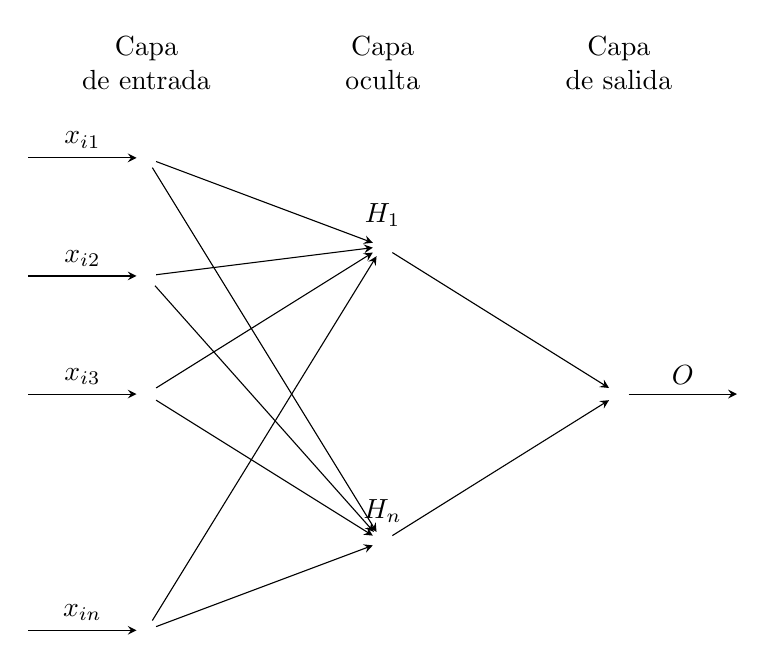
\begin{tikzpicture}[x=1.5cm, y=1.5cm, >=stealth]

\foreach \m/\l [count=\y] in {1,2,3,missing,4}
  \node [every neuron/.try, neuron \m/.try] (input-\m) at (0,2.5-\y) {};

\foreach \m [count=\y] in {1,missing,2}
  \node [every neuron/.try, neuron \m/.try ] (hidden-\m) at (2,2-\y*1.25) {};

\foreach \m [count=\y] in {1}
  \node [every neuron/.try, neuron \m/.try ] (output-\m) at (4,0.5-\y) {};

\foreach \l [count=\i] in {1,2,3,n}
  \draw [<-] (input-\i) -- ++(-1,0)
    node [above, midway] {$x_{i\l}$};

\foreach \l [count=\i] in {1,n}
  \node [above] at (hidden-\i.north) {$H_\l$};

\foreach \l [count=\i] in {1}
  \draw [->] (output-\i) -- ++(1,0)
    node [above, midway] {$O$};

\foreach \i in {1,...,4}
  \foreach \j in {1,...,2}
    \draw [->] (input-\i) -- (hidden-\j);

\foreach \i in {1,...,2}
  \foreach \j in {1}
    \draw [->] (hidden-\i) -- (output-\j);

\foreach \l [count=\x from 0] in {de entrada, oculta, de salida}
  \node [align=center, above] at (\x*2,2) {Capa \\ \l};

\end{tikzpicture}
    \caption{Red neuronal prealimentada con una capa oculta}
    \label{fig:mlp}
\end{figure}

Una red neuronal prealimentada, conocida históricamente también como perceptrón multicapa, es un sistema de componentes 
de procesamiento de varias capas, como el descrito en la figura \ref{fig:mlp}. La primera capa de esta red se le llama 
capa de entrada y es la que recibe los datos, todas las intermedias son denominadas capas ocultas y la última es 
denominada capa de salida. Gracias a estas capas ocultas, la red puede extraer resultados más complejos a partir de los 
datos. En un sentido poco formal, podemos decir que mediante este aumento de dimensiones de interacción entre neuronas, 
la red obtiene una perspectiva ``global'' \cite{haykin_1999}. 

\vspace{10pt}
Las redes neuronales prealimentadas son capaces de 
resolver problemas de aprendizaje automático mediante \textit{aprendizaje supervisado}. En este tipo de aprendizaje, el 
modelo recibe como conjunto de entrenamiento datos etiquetados previamente y realiza predicciones de las etiquetas de 
los ejemplos \cite{mohri_rostamizadeh_talwalkar_2018}.

\vspace{10pt}
En las redes neuronales prealimentadas, cada neurona está conectada con todas las neuronas de las capas vecinas, y un 
peso es asignado a cada una de esas conexiones. Estas neuronas nunca están conectadas a otras neuronas de su misma capa
ni a neuronas de capas que no son adyacentes. Además, las conexiones a la capa anterior son siempre de entrada, funcionando como conexiones de salida las que se conectan con la siguiente capa. Los datos de entrada son suministrados 
a la capa de entrada, y son procesados de manera ascendente en las capas hasta llegar a la salida \cite{Yagawa2021}. Es 
por este camino que toman los datos (de izquierda a derecha y en una única dirección) por lo que se las denomina redes 
neuronales prealimentadas, \textit{feed-foward neural networks} en inglés. 

% -------------------------------------------------------------------------------------------------------------------
\subsection{Neuronas}

Veamos ahora de qué se compone una neurona y cuál es su funcionamiento. Identificamos tres elementos básicos de las
neuronas de una red:
\begin{enumerate}
    \item Un conjunto de conexiones o \textit{sinapsis} con un peso asignado a cada una de ellas, es decir, para un
    valor de entrada de una conexión $x_j$ a una neurona $k$, ese valor es multiplicado por un peso $w_{kj}$.
    \item Una función de adición o \textit{combinador lineal} que realiza una suma ponderada de todos los valores de 
    entrada de la neurona, utilizando sus respectivos pesos. Para una neurona $k$, se describe esta función de la
    siguiente manera:
    \begin{equation}\label{eq:neurona}
        u_k(x)=\sum_{j=1}^mw_{kj}x_j+b_k
    \end{equation}
    donde
    \begin{description}
        \item[$m$] es el número de conexiones de entrada de la neurona.
        \item[$x=(x_1,\dots,x_m)$] son los valores de entrada.
        \item[$w_{k1},\dots,w_{km}$] son los pesos de las conexiones.
        \item[$b_k$] es un valor de sesgo para la neurona.
    \end{description}
    El valor de sesgo de la neurona es esencial, ya que sin él el hiperplano generado por la función incluye siempre el
    origen de coordenadas, limitando la variabilidad y la capacidad de aprendizaje de la neurona. Si añadimos una nueva 
    conexión, cuyo valor de entrada sea $x_0=1$ y su peso $w_{k0}=b_k$, podemos reescribir la ecuación anterior de la 
    siguiente manera:
    \begin{equation}
        v_k(x)=\sum_{j=0}^mw_{kj}x_j
    \end{equation}
    \item Una \textit{función de activación} $\varphi$ que acota la amplitud de la salida de la neurona. Esta 
    función transforma los valores de salida del combinador lineal a valores dentro de un intervalo mucho más 
    pequeño. Los intervalos más usuales suelen ser $[0,1]$ y $[-1,1]$. Para eliminar la linealidad de las redes, 
    normalmente se suelen utilizar como funciones de activación la función sigmoide y la tangente hiperbólica, que justamente acotan la salida de la neurona a los intervalos $[0,1]$ y $[-1,1]$, respectivamente. Estas funciones 
    tienen la siguiente expresión:
    \begin{equation}
        \text{sigmoide}(v)=\frac{1}{1+e^{-v}}\quad\quad\tanh(v)=\frac{e^v-e^{-v}}{e^v+e^{-v}}
    \end{equation}
    Al resultado de aplicar la función de activación a la neurona se le suele denotar como $\tilde{y}_k$.
\end{enumerate}

Un esquema de estas neuronas es el de la figura \ref{fig:neurona} \cite{haykin_1999}.

\begin{figure}[htbp!]
    \centering
    \begin{tikzpicture}[x=1.cm, y=1.5cm, >=stealth]

\foreach \m/\l [count=\y] in {1,2,3,missing,4}
  \node [every neuron/.try, neuron \m/.try, draw=none] (input-\m) at (0,2.5-\y) {};

\foreach \m [count=\y] in {1}
  \node [semi,shape border rotate=90] (output-\m) at (2,0.5-\y) {$\sum$};
  \node [semi,right=0cm of output-1,shape border rotate=270] (output-f) {$\varphi$};

\foreach \l [count=\i] in {1,2,3,j}
  \draw (input-\i) ++(0,0)
    node {$x_\l$};

\foreach \l [count=\i] in {f}
  \draw [->] (output-\l) -- ++(1,0)
    node [above, midway] {$\tilde{y}_k$};

\foreach \i in {1,...,4}
  \foreach \j in {1}
    \draw [->] (input-\i) -- (output-\j);
\end{tikzpicture}
    \caption{Esquema de una neurona}
    \label{fig:neurona}
\end{figure}

\vspace{10pt}
Existen ciertas particularidades para las neuronas de la capa de entrada y las de la capa de salida. Las neuronas de la
capa de entrada tienen únicamente una conexión de entrada, que se corresponde al valor de una de las características de
los ejemplos. Tampoco se le suele asignar un peso a este valor de entrada, y como función de activación se utiliza la
función identidad \cite{Yagawa2021}. Para las neuronas de la capa de salida, si se trata de un problema de regresión,
suele también utilizarse la función de identidad como función de activación, puesto que usualmente el valor a predecir
no suele estar acotado al intervalo unidad. En los problemas de clasificación, se utiliza una función umbral para
asignar la categoría al resultado de la suma ponderada \cite{mlp}. Esta función tiene la siguiente expresión:
\begin{equation}
    f(v)=\begin{cases}
        1 & \text{si}\quad v>0.5 \\
        -1 & \text{en cualquier otro caso} 
    \end{cases}
\end{equation}


% -------------------------------------------------------------------------------------------------------------------
\subsection{Predicciones, medidas de rendimiento y algoritmo de aprendizaje}

\subsubsection*{Predicciones}

El objetivo de una red prealimentada es realizar predicciones a partir de un conjunto de datos de entrada. Para 
realizar una de estas predicciones, se utiliza la \textit{propagación hacia delante}, que no es más que, a partir de
los datos de entrada, calcular los valores de salida de las neuronas capa a capa hasta llegar a la capa final. 
Supongamos que tenemos una red con dos neuronas de entrada, tres neuronas en una capa oculta y una neurona en la capa
de salida, y se trata de una red que pretende clasificar. Sea $x=(x_1,x_2)$ un ejemplo, y denotando con un superíndice 
la capa de la neurona y con un subíndice la neurona de esa capa, podemos predecir su etiqueta de la siguiente manera:
\begin{enumerate}
    \item Para la capa de entrada, su salida serán los mismos datos de entrada. Por tanto, si denotamos la salida de esta capa como $x^{(1)}$, $x^{(1)}_1=x_1$ y $x^{(1)}_2=x_1$.
    \item Para la capa oculta, la salida de cada neurona $k$ la calculamos como:
    \begin{equation}
        x^{(2)}_k=\varphi(\sum_{i=0}^2w^{(2)}_{kj}x^{(1)}_i)
    \end{equation}
    \item Finalmente, la predicción de la red sera, utilizando la capa de salida y denotando la función umbral por $f$:
    \begin{equation}
        \tilde{y}=f(\varphi(\sum_{i=0}^3w^{(3)}_jx^{(2)}_i))
    \end{equation}
\end{enumerate}

Podemos ver, de esta manera, que toda red neuronal puede ser representada como una composición de funciones donde capa
etapa está anidada en la siguiente etapa. La propagación hacia delante es un paso indispensable para el posterior 
cálculo de las medidas de rendimiento, que a su vez son utilizadas por los algoritmos de aprendizaje para mejorar la 
calidad de las predicciones\cite{mlp}. 

\subsubsection*{Medidas de rendimiento}

Para determinar el rendimiento de la red, se utilizan medidas que llamaremos \textit{funciones de coste}, 
\textit{funciones de pérdida} o \textit{funciones objetivo}. Convencionalmente, se llama \textit{funciones de pérdida} 
a la medida de error de un ejemplo de entrenamiento, \textit{función de coste} a la agregación de las funciones de 
pérdida del conjunto de entrenamiento completo y \textit{función objetivo} a la medida general del error en la red 
\cite{mlp}. 

\vspace{10pt}
Las funciones de coste son utilizadas por los algoritmos de aprendizaje para conocer la ``bondad'' de las predicciones 
durante el entrenamiento. La función de coste más usual es el error cuadrático medio, que tiene la siguiente expresión:
\begin{equation}
    \text{MSE}=\frac 1n\sum_{i=1}^n(y_i-\tilde{y}_i)^2
\end{equation}
donde $n$ es el conjunto de ejemplos de entrenamiento, $y_i$ las etiquetas de cada ejemplo y $\title{y}_i$ las 
predicciones de la red de cada ejemplo.

\vspace{10pt}
Para los problemas de clasificación, una de las maneras más exhaustivas de representar el rendimiento de la red es la
matriz de confusión. Se trata de una matriz $2\times 2$, donde las filas se corresponden a las posibles categorías y
las columnas a las categorías predichas. De esta manera, los valores estimados correctamente por el modelo son los de 
la diagonal principal, mientras que las predicciones erróneas se corresponden a la diagonal secundaria 
\cite{muller_guido_2017}. Si definimos las categorías como ``positiva'' y ``negativa'', la matriz de confusión se puede 
representar como la figura \ref{fig:conf-mat}. 

\begin{figure}[htb!]
    \centering
    \begin{tikzpicture}[
box/.style={draw,rectangle,minimum size=3cm,text width=2.5cm,align=left}]
\matrix (conmat) [row sep=.1cm,column sep=.1cm] {
\node (tpos) [box,
    label=left:\( \mathbf{p} \),
    label=above:\( \mathbf{\tilde{p}} \),
    ] {Verdaderos \\ positivos \\ (VP)};
&
\node (fneg) [box,
    label=above:\( \mathbf{\tilde{n}} \),
    label=above right:\textbf{total},
    label=right:\( \mathrm{P} \)] {Falsos \\ negativos \\ (FN)};
\\
\node (fpos) [box,
    label=left:\( \mathbf{n} \),
    label=below left:\textbf{total},
    label=below:\( \mathrm{\tilde{P}} \)] {Falsos \\ positivos \\ (FP)};
&
\node (tneg) [box,
    label=right:\( \mathrm{N} \),
    label=below:\( \mathrm{\tilde{N}} \)] {Verdaderos \\ negativos \\ (VN)};
\\
};
\node  [rotate=90,left=.05cm of conmat,anchor=center,text width=1.5cm,align=center] {\textbf{Etiquetas \\ reales}};
\node [above=.05cm of conmat] {\textbf{Etiquetas predichas}};
\end{tikzpicture}
    \caption{Matriz de confusión}
    \label{fig:conf-mat}
\end{figure}

\vspace{10pt}
Podemos abreviar los elementos de la matriz por sus iniciales. Notaremos VP a los verdaderos positivos, FP a los falsos
positivos, VN a los verdaderos negativos y FN a los falsos negativos. A partir de la matriz de confusión, podemos 
definir medidas concretas que resumen la información proporcionada por la misma:

\vspace{10pt}\textbf{\textit{Exactitud}}: La exactitud o \textit{accuracy} representa 
el porcentaje de predicciones correctas realizadas por el modelo. Se calcula de la 
siguiente manera.
\begin{equation}
    \text{\textit{Exactitud}}=\frac{VP+VN}{VP+VN+FP+FN}
    =\frac{VP+VN}{P+N}=\frac{VP+VN}{\tilde{P}+\tilde{N}}
\end{equation}

\vspace{10pt}\textbf{\textit{Precisión}}: La \textit{precision}, en castellano precisión, mide la relación entre los
verdaderos positivos y el total de positivos, y tiene la siguiente expresión:
\begin{equation}
    \text{\textit{Precisión}}=\frac{VP}{VP+FP}=\frac{VP}{\tilde{P}}
\end{equation}
Esta medida suele utilizarse cuando es importante para el modelo minimizar el número de falsos positivos. Se le puede
denominar también como \textit{valor predictivo positivo} (\textit{positive predictive value} en inglés).

\vspace{10pt}\textbf{\textit{Sensibilidad}}: La sensibilidad o \textit{recall} es una medida que permite calcular el 
porcentaje de verdaderos positivos sobre el total de predicciones positivas. Se calcula como:
\begin{equation}
    \text{\textit{Sensibilidad}}=\frac{VP}{VP+FN}=\frac{VP}{P}
\end{equation}
A diferencia de la precisión, esta medida es importante cuando queremos evitar los falsos negativos. Es conocida también
como \textit{ratio de verdaderos positivos}.

\vspace{10pt}\textbf{\textit{$f_1$-score}}: El \textit{$f_1$-score} o puntuación $f_1$ es una medida que combina la
precisión y la sensibilidad. En particular, se trata de la media armónica de esas dos medidas:
\begin{equation}
    f_1=\frac{\text{\textit{Sensibilidad}}
\cdot\text{\textit{Precisión}}}{\text{\textit{Sensibilidad}}+\text{\textit{Precisión}}}
\end{equation}
La puntuación $f_1$ suele ser utilizada para medir la bondad de la red cuando el conjunto de datos sobre el que estamos
trabajando posee un número desequilibrado de ejemplos de cada categoría \cite{muller_guido_2017}.

\subsubsection*{Algoritmo de aprendizaje}

Para poder realizar predicciones adecuadas, una red neuronal necesita un algoritmo de aprendizaje que modifique los
pesos de sus neuronas a partir de la función de coste utilizada. Un algoritmo de aprendizaje se compone de las 
siguientes etapas:
\begin{enumerate}
    \item \textbf{Inicialización}: En este paso, todos los pesos de la red son inicializados con valores aleatorios.
    Debido a esta aleatoriedad, normalmente se realizan varios entrenamientos del modelo y se toma el que de mejores
    resultados.
    \item \textbf{Propagación hacia delante}: Se realiza la predicción de ejemplos de entrenamiento mediante la
    propagación hacia delante, cuyo funcionamiento hemos descrito.
    \item \textbf{Propagación hacia atrás o retropropagación}: Utilizando las predicciones del paso anterior, y 
    mediante el uso de una función de costo, se modifican los valores de los pesos y sesgo en orden descendente. Después, se pasa al paso 2 de nuevo y así de forma repetitiva hasta que se cumple una condición de salida, como 
    puede ser el número de veces que se utiliza el conjunto de datos completo (épocas), el número total de veces que se ejecuta la retropropagación (nº de iteraciones), valor umbral de error, \dots El algoritmo tradicionalmente 
    utilizado para esta fase es el descenso de gradiente. Este método modifica los pesos de la red de la siguiente 
    manera:
    \begin{gather}
        \Delta w^{(p)}_{ji}=-\frac{\partial E}{\partial w^{(p)}_{ji}} \\
        w^{(p)}_{ji}=w^{(p)}_{ji}+\alpha\cdot\Delta w^{(p)}_{ji}
    \end{gather}
    donde $\Delta w^{(p)}_{ji}$ es la modificación del peso $i$-ésimo de la neurona $j$ de la capa $p$, $E$ es la
    función de costo y $\alpha$ es un parámetro, llamado ratio de aprendizaje, que escala la modificación de los
    pesos \cite{Yagawa2021}.\\
    Existen multitud de algoritmos aparte del descenso de gradiente, optimizados para cierto tipo de redes, conjuntos
    de datos o recursos computacionales. En este trabajo, se utiliza para las redes el algoritmo de optimización por
    enjambre de partículas, definido más adelante.
\end{enumerate}

% -------------------------------------------------------------------------------------------------------------------
\section{Aproximadores universales}

Una pregunta que puede surgir acerca de las redes neuronales prealimentadas es, ¿son capaces estos modelos de resolver
o aproximarse a la solución de los problemas para los cuales han sido creadas? Todo problema de aprendizaje automático
lo podemos ver como la búsqueda de una función tal que, tomando como entrada la información de la que disponemos, 
sea capaz de dar la solución o predicción correcta siempre. Por ejemplo, que sea capaz de determinar el diagnóstico
correcto siempre a partir de datos médicos. A esta función se la suele denominar \textit{función objetivo}. 

\vspace{10pt}
En 1989 Kurt Hornik, Maxwell Stinchcombe y Halbert White demostraron que toda red neuronal prealimentada es un 
aproximador universal. En particular, demostraron que:
\begin{quote}
    Las redes neuronales prealimentadas con al menos una capa oculta usando una función de activación sigmoidea 
    arbitraria son capaces de aproximar cualquier función boreliana medible que vaya de un espacio de dimensión finita 
    a otro con el grado de precisión que se desee, siempre que haya suficientes capas ocultas. En este sentido, las 
    redes neuronales prealimentadas son aproximadores universales. \cite{hornik_1989}
\end{quote}
Poco después, en 1991, Hornik demostró que no es necesario que la función de activación sea sigmoidea para considerar 
estas redes como aproximadores universales. Veamos unas pinceladas de este trabajo, puesto que para mostrar las 
pruebas completas es necesario utilizar conceptos avanzados del análisis funcional. Para ello, vamos a trabajar con 
una red neuronal prealimentada con una única capa oculta y una única neurona de salida, que es justamente el tipo de 
neuronas implementadas en este trabajo. Entonces, el conjunto de funciones que implementan esas redes, con $n$ neuronas 
ocultas es
\begin{equation}
    \mathfrak{R}_k^{(n)}(\varphi)=\Big\{h:\mathbb{R}^k\to\mathbb{R}\mid h(x)=f(\sum_{j=1}^n\varphi(w_j^Tx+b_j))\Big\}
\end{equation}
donde $\varphi$ es la función de activación común para todas las neuronas y $T$ denota la transposición de forma que si
$w_j=(w_{j1},\dots,w_{jk})$ y $x=(x_1,\dots,x_k)$, $w_j^Tx$ denota el producto escalar \cite{hornik_1991}. Podemos ver 
que la notación $w_j^Tx+b_j$ es equivalente a la de la ecuación \eqref{eq:neurona}. El conjunto de todas las funciones
implementadas por este tipo de red con un número arbitrariamente grande de neuronas ocultas es entonces:
\begin{equation}
    \mathfrak{R}_k(\varphi)=\bigcup_{n=1}^\infty\mathfrak{R}_k^{(n)}(\varphi)
\end{equation}

Definimos ahora el espacio de funciones en el cual se encuentran nuestros modelos. Sea $\mu$ una medida, para 
$1\leq p<\infty$ definimos la norma:
\begin{equation}
    \|f\|_{p,\mu}=\Big[\int_{\mathbb{R}^k}|f(x)|^pd\mu(x)\Big]^{\frac 1p}
\end{equation}

\begin{definicion}$L^p(\mu)$ es el espacio de funciones $f$ tal que $\|f\|_{p,\mu}<\infty$. Diremos que 
$S\subset L^p(\mu)$ es \textit{denso} en $L^p(\mu)$ si para cualquier $f\in L^p(\mu)$ y $\epsilon>0$, existe una función
$g\in S$ tal que $\|f-g\|_{p,\mu}<\epsilon$.
\end{definicion}

Con estas definiciones, llegamos a un primer resultado:

\begin{teorema}Si $\varphi$ es no constante y no acotada, entonces $\mathfrak{R}_k(\varphi)$ es denso en $L^p(\mu)$ 
para todas las medidas $\mu$ finitas en $\mathbb{R}^k$ \cite{hornik_1991}.
\end{teorema}

Tenemos entonces que toda red neuronal prealimentada es densa en $L^p(\mu)$, es decir, podemos aproximar cualquier
función de $L^p(\mu)$ mediante una red neuronal. Si ahora definimos, para $1\leq p<\infty$, la norma
\begin{equation}
    \|f\|_p=\Big[\int_{\mathbb{R}^k}|f(x)|^pdx\Big]^{\frac 1p}
\end{equation}
y denotamos $C(X)$ como el espacio de todas las funciones $f$ continuas en $X\subseteq\mathbb{R}^k$, entonces 
$S\subset C(X)$ es \textit{denso} en $C(X)$ si para cualquier $f\in C(X)$ y $\epsilon>0$, existe una función $g\in S$ 
tal que $\|f-g\|_p<\epsilon$. Podemos ahora dar un resultado equivalente al anterior pero para funciones continuas:

\begin{teorema}Si $\varphi$ es no constante y no acotada, entonces $\mathfrak{R}_k(\varphi)$ es denso en $C(X)$
para todos los subconjuntos compactos $X$ de $\mathbb{R}^k$ \cite{hornik_1991}.
\end{teorema}

Veamos ahora que podemos tomar $\varphi$ acotada y llegar a los mismos resultados. Para ello, vamos a definir algunos
conceptos. En primer lugar sea una $k$-tupla $\alpha=(\alpha_1,\dots,\alpha_k)$ de enteros no negativos, denominamos
\textit{orden} de $\alpha$ a $|\alpha|=\alpha_1+\cdots +\alpha_k$ y, para una función $f$ de $\mathbb{R}^k$, escribimos
su correspondiente derivada parcial como:
\begin{equation}
    D^\alpha f(x)=\frac{\partial^{\alpha_1+\cdots+\alpha_n}f}{\partial x_1^{\alpha_1}\cdots\partial x_k^{\alpha_k}}(x)
\end{equation}
Definimos ahora $C^m(\mathbb{R}^k)$ como el espacio de todas las funciones $f$ que, junto con sus derivadas parciales 
$D^\alpha f$ de orden $|\alpha|\leq m$, son continuas en $\mathbb{R}^k$. Definimos para $f\in C^m(\mathbb{R}^k)$ la
norma:
\begin{equation}
    \|f\|_{m}:=\max_{|\alpha|\leq m}\sup_{x\in\mathbb{R}^k}|D^\alpha f(x)|
\end{equation}
Diremos que $S\subset C^m(\mathbb{R}^k)$ es \textit{uniformemente $m$-denso sobre compactos} en $C^m(\mathbb{R}^k)$ si
para toda $f\in C^m(\mathbb{R}^k)$ y para todo $\epsilon>0$, existe una función $g\in S$ tal que $\|f-g\|_m<\epsilon$
\cite{hornik_1991}.

\vspace{10pt}
Ahora, sea $f\in  C^m(\mathbb{R}^k)$, $\mu$ una medida finita en $\mathbb{R}^k$ y $1\leq p<\infty$, definimos la norma
\begin{equation}
    \|f\|_{m,p}:=\Big[\sum_{|\alpha|\leq m}\int_{\mathbb{R}^k}|D^\alpha f|^pd\mu\Big]^{\frac 1p}
\end{equation}
y el espacio $C^{m,p}(\mu)$ como
\begin{equation}
    C^{m,p}(\mu)=\{f\in C^m(\mathbb{R}^k)\mid \|f\|_{m,p}<\infty\}
\end{equation}
Podemos ver que $C^{m,p}(\mu)=C^m(\mathbb{R}^k)$ si $\mu$ tiene soporte compacto. Diremos que $S$ es \textit{denso} en
$C^{m,p}(\mu)$ si para toda $f\in C^m(\mathbb{R}^k)$ y para todo $\epsilon>0$, existe una función $g\in S$ tal que
$\|f-g\|_{m,p}<\epsilon$ \cite{hornik_1991}. Tenemos, utilizando estas definiciones, los siguientes resultados:

\begin{teorema}Si $\varphi\in C^m(\mathbb{R}^k)$ es no constante y acotada, entonces $\mathfrak{R}_k(\varphi)$ es
uniformemente $m$-denso sobre compactos en $C^m(\mathbb{R}^k)$ y denso en $C^{m,p}(\mu)$ para todas las medidas finitas
de $\mathbb{R}^k$ con soporte compacto \cite{hornik_1991}.
\end{teorema}

Este resultado proporciona la justificación del uso de, por ejemplo, la tangente hiperbólica como función de activación.
Puesto que $\tanh\in C^\infty(\mathbb{R})$, entonces podemos resolver cualquier problema de aprendizaje cuya función
objetivo pertenezca a $C^m(\mathbb{R}^k)$.

\begin{teorema}Si $\varphi\in C^m(\mathbb{R}^k)$ es no constante y todas sus derivadas hasta orden $m$ son acotadas,
entonces $\mathfrak{R}_k(\varphi)$ es denso en $C^{m,p}(\mu)$ para todas las medidas finitas de $\mathbb{R}^k$ con 
soporte compacto \cite{hornik_1991}.
\end{teorema}

De esta manera, es fácil observar que las redes neuronales prealimentadas con al menos una capa oculta son, bajo 
condiciones muy generales sobre la función de activación de las neuronas ocultas, aproximadores universales, siempre y 
cuando la red tenga un número suficientemente grande de neuronas ocultas. Es importante notar que estos resultados no 
dan ninguna indicación constructiva, es decir, no proporcionan ninguna información acerca del número de capas ocultas, 
el número de neuronas ocultas o la función $\varphi$ más indicada para la aproximación \cite{hornik_1991}. Es por ello 
que, aunque tengamos la certeza de poder obtener un modelo que se aproxime casi a la perfección a la solución del 
problema, es necesario y recomendable realizar pruebas sobre los modelos modificando sus parámetros (número de neuronas 
de la capa oculta, iteraciones en el proceso de aprendizaje, \dots) para intentar encontrar ese teórico que aproxima la solución.

% -------------------------------------------------------------------------------------------------------------------
\section{Implementación}

Para construir las redes neuronales prealimentadas con una única capa oculta utilizadas en la herramienta, se ha 
utilizado una \textit{interfaz} de Scala (\texttt{trait}), que contiene la estructura común para tanto los 
clasificadores como los regresores. El código de esta interfaz se encuentra en el apéndice \ref{ap:estructura_ann},
así como el de las clases específicas. Este esqueleto para redes neuronales contiene:

\subsubsection*{Variables}
\begin{itemize}
    \item El número de neuronas de entrada y ocultas.
    \item Los conjuntos de ejemplos para entrenamiento y para test.
    \item Los pesos de la red.
    \item El objeto que calcula el error cuadrático medio de la red.
    \item El objeto que realiza la propagación hacia delante de la red.
    \item El objeto que contiene el algoritmo de aprendizaje de la red.
\end{itemize}
\subsubsection*{Métodos}
\begin{itemize}
    \item Una función para proporcionar el conjunto de datos de entrenamiento (en formato \texttt{csv}).
    \item Un método que asigna el conjunto de datos de test a partir de un fichero (en formato \texttt{csv}).
    \item Una función asigna a la red una instancia de una clase que implementa un algoritmo de aprendizaje.
    \item Un método para realizar el proceso de aprendizaje, usando como criterio de parada un número de 
    iteraciones.
    \item Una función que predice la etiqueta de un ejemplo dado.
    \item Un método que realiza la predicción de etiquetas del conjunto de datos de test.
    \item Una función que calcula el error cuadrático medio de la red con el conjunto de datos de test.
    \item Un método que exporta los pesos a un archivo (en formato \texttt{csv}).
\end{itemize}

A partir de la interfaz, se construyen dos clases, \texttt{Classifier} y \texttt{Regressor}, que implementan las
particularidades de esos tipos de redes, como son la función de propagación hacia delante o el preprocesamiento de
los datos de entrada. Finalmente, se construyó una interfaz para la incorporación de algoritmos de aprendizaje a las
redes de la librería, denominada \texttt{Trainer}.

\endinput
%--------------------------------------------------------------------
% FIN DEL CAPÍTULO. 
%--------------------------------------------------------------------

% !TeX root = ../tfg.tex
% !TeX encoding = utf8

\chapter{Paralelismo}\label{chap:paralel}

El \textit{paralelismo} o \textit{concurrencia} en el proceso de aprendizaje de las redes es el elemento clave a la
hora de minimizar el tiempo de ejecución del entrenamiento de los modelos. Un programa puede, normalmente, dividirse
en muchos componentes que denominamos \textit{tareas}. Un \textit{programa concurrente} es aquel que consiste en un
número de tareas computacionales que pueden ser ejecutadas paralelamente. El programa concurrente define cómo las 
tareas se comunican y cooperan entre sí, además de sincronizar, o no, sus acciones \cite{czech_2017}. 

\vspace{10pt}
Supongamos que tenemos un programa $O$ con siete tareas $o_i$. Es fácil ver cómo el paralelizar procesos ahorra tiempo
de ejecución, como se muestra en las figuras \ref{fig:prog-sec} y \ref{fig:prog-par} (donde $p$ denota procesador).
Podemos observar que, al ser ejecutados de forma simultánea, algunas de las tareas se solapan en el tiempo, acortando 
el tiempo total necesario para la computación del programa \cite{czech_2017}.

\begin{figure}[htbp!]
    \centering
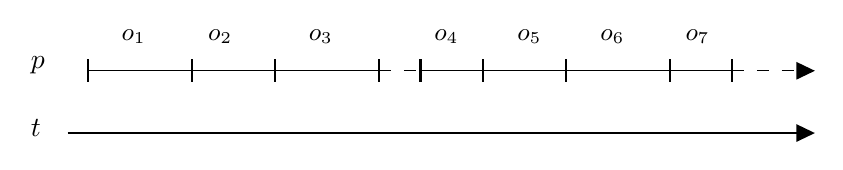
\begin{tikzpicture}[x=0.75pt,y=0.75pt,yscale=-1,xscale=1]
%uncomment if require: \path (0,300); %set diagram left start at 0, and has height of 300
%Straight Lines [id:da7449676638708221] 
\draw    (50,50) -- (72.42,50) -- (100,50) ;
\draw [shift={(100,50)}, rotate = 180] [color={rgb, 255:red, 0; green, 0; blue, 0 }  ][line width=0.75]    (0,5.59) -- (0,-5.59)   ;
\draw [shift={(50,50)}, rotate = 180] [color={rgb, 255:red, 0; green, 0; blue, 0 }  ][line width=0.75]    (0,5.59) -- (0,-5.59)   ;
%Straight Lines [id:da9687422174007011] 
\draw    (100,50) -- (122.42,50) -- (140,50) ;
\draw [shift={(140,50)}, rotate = 180] [color={rgb, 255:red, 0; green, 0; blue, 0 }  ][line width=0.75]    (0,5.59) -- (0,-5.59)   ;
\draw [shift={(100,50)}, rotate = 180] [color={rgb, 255:red, 0; green, 0; blue, 0 }  ][line width=0.75]    (0,5.59) -- (0,-5.59)   ;
%Straight Lines [id:da27287006149854454] 
\draw    (140,50) -- (162.42,50) -- (190,50) ;
\draw [shift={(190,50)}, rotate = 180] [color={rgb, 255:red, 0; green, 0; blue, 0 }  ][line width=0.75]    (0,5.59) -- (0,-5.59)   ;
\draw [shift={(140,50)}, rotate = 180] [color={rgb, 255:red, 0; green, 0; blue, 0 }  ][line width=0.75]    (0,5.59) -- (0,-5.59)   ;
%Straight Lines [id:da5536134933880722] 
\draw    (210,50) -- (232.42,50) -- (240,50) ;
\draw [shift={(240,50)}, rotate = 180] [color={rgb, 255:red, 0; green, 0; blue, 0 }  ][line width=0.75]    (0,5.59) -- (0,-5.59)   ;
\draw [shift={(210,50)}, rotate = 180] [color={rgb, 255:red, 0; green, 0; blue, 0 }  ][line width=0.75]    (0,5.59) -- (0,-5.59)   ;
%Straight Lines [id:da753886597033629] 
\draw    (240,50) -- (262.42,50) -- (280,50) ;
\draw [shift={(280,50)}, rotate = 180] [color={rgb, 255:red, 0; green, 0; blue, 0 }  ][line width=0.75]    (0,5.59) -- (0,-5.59)   ;
\draw [shift={(240,50)}, rotate = 180] [color={rgb, 255:red, 0; green, 0; blue, 0 }  ][line width=0.75]    (0,5.59) -- (0,-5.59)   ;
%Straight Lines [id:da5516104166014002] 
\draw    (280,50) -- (302.42,50) -- (305.58,50) -- (330,50) ;
\draw [shift={(330,50)}, rotate = 180] [color={rgb, 255:red, 0; green, 0; blue, 0 }  ][line width=0.75]    (0,5.59) -- (0,-5.59)   ;
\draw [shift={(280,50)}, rotate = 180] [color={rgb, 255:red, 0; green, 0; blue, 0 }  ][line width=0.75]    (0,5.59) -- (0,-5.59)   ;
%Straight Lines [id:da8194201143798694] 
\draw    (330,50) -- (352.42,50) -- (360,50) ;
\draw [shift={(360,50)}, rotate = 180] [color={rgb, 255:red, 0; green, 0; blue, 0 }  ][line width=0.75]    (0,5.59) -- (0,-5.59)   ;
\draw [shift={(330,50)}, rotate = 180] [color={rgb, 255:red, 0; green, 0; blue, 0 }  ][line width=0.75]    (0,5.59) -- (0,-5.59)   ;
%Straight Lines [id:da65503157723167] 
\draw  [dash pattern={on 4.5pt off 4.5pt}]  (360,50) -- (397,50) ;
\draw [shift={(400,50)}, rotate = 180] [fill={rgb, 255:red, 0; green, 0; blue, 0 }  ][line width=0.08]  [draw opacity=0] (8.93,-4.29) -- (0,0) -- (8.93,4.29) -- cycle    ;
%Straight Lines [id:da7036502375733221] 
\draw    (40,80) -- (397,80) ;
\draw [shift={(400,80)}, rotate = 180] [fill={rgb, 255:red, 0; green, 0; blue, 0 }  ][line width=0.08]  [draw opacity=0] (8.93,-4.29) -- (0,0) -- (8.93,4.29) -- cycle    ;
%Straight Lines [id:da7413442953095534] 
\draw  [dash pattern={on 4.5pt off 4.5pt}]  (190,50) -- (210,50) ;

% Text Node
\draw (21,42) node [anchor=north west][inner sep=0.75pt]   [align=left] {$\displaystyle p$};
% Text Node
\draw (73.83,38.13) node [anchor=south] [inner sep=0.75pt]  [font=\small] [align=left] {$\displaystyle o_{1} \ $};
% Text Node
\draw (115.5,38) node [anchor=south] [inner sep=0.75pt]  [font=\small] [align=left] {$\displaystyle o_{2} \ $};
% Text Node
\draw (164,38) node [anchor=south] [inner sep=0.75pt]  [font=\small] [align=left] {$\displaystyle o_{3} \ $};
% Text Node
\draw (224.5,38) node [anchor=south] [inner sep=0.75pt]  [font=\small] [align=left] {$\displaystyle o_{4} \ $};
% Text Node
\draw (264.5,38) node [anchor=south] [inner sep=0.75pt]  [font=\small] [align=left] {$\displaystyle o_{5} \ $};
% Text Node
\draw (304.5,38) node [anchor=south] [inner sep=0.75pt]  [font=\small] [align=left] {$\displaystyle o_{6} \ $};
% Text Node
\draw (345.5,38) node [anchor=south] [inner sep=0.75pt]  [font=\small] [align=left] {$\displaystyle o_{7} \ $};
% Text Node
\draw (21,72) node [anchor=north west][inner sep=0.75pt]   [align=left] {$\displaystyle t$};
\end{tikzpicture}
    \caption{Programa ejecutado en un procesador $p$ secuencialmente.}
    \label{fig:prog-sec}
\end{figure}

\begin{figure}[htbp!]
    \centering
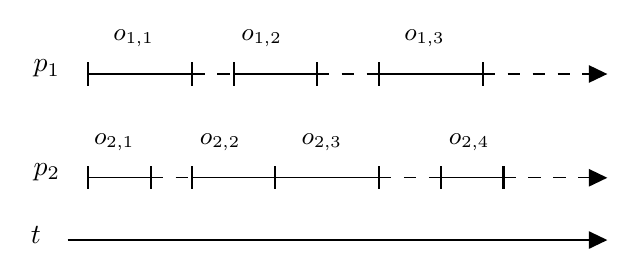
\begin{tikzpicture}[x=0.75pt,y=0.75pt,yscale=-1,xscale=1]
%uncomment if require: \path (0,300); %set diagram left start at 0, and has height of 300

%Straight Lines [id:da7449676638708221] 
\draw    (50,50) -- (72.42,50) -- (100,50) ;
\draw [shift={(100,50)}, rotate = 180] [color={rgb, 255:red, 0; green, 0; blue, 0 }  ][line width=0.75]    (0,5.59) -- (0,-5.59)   ;
\draw [shift={(50,50)}, rotate = 180] [color={rgb, 255:red, 0; green, 0; blue, 0 }  ][line width=0.75]    (0,5.59) -- (0,-5.59)   ;
%Straight Lines [id:da9687422174007011] 
\draw    (120,50) -- (142.42,50) -- (160,50) ;
\draw [shift={(160,50)}, rotate = 180] [color={rgb, 255:red, 0; green, 0; blue, 0 }  ][line width=0.75]    (0,5.59) -- (0,-5.59)   ;
\draw [shift={(120,50)}, rotate = 180] [color={rgb, 255:red, 0; green, 0; blue, 0 }  ][line width=0.75]    (0,5.59) -- (0,-5.59)   ;
%Straight Lines [id:da27287006149854454] 
\draw    (190,50) -- (212.42,50) -- (240,50) ;
\draw [shift={(240,50)}, rotate = 180] [color={rgb, 255:red, 0; green, 0; blue, 0 }  ][line width=0.75]    (0,5.59) -- (0,-5.59)   ;
\draw [shift={(190,50)}, rotate = 180] [color={rgb, 255:red, 0; green, 0; blue, 0 }  ][line width=0.75]    (0,5.59) -- (0,-5.59)   ;
%Straight Lines [id:da7036502375733221] 
\draw    (40,130) -- (297,130) ;
\draw [shift={(300,130)}, rotate = 180] [fill={rgb, 255:red, 0; green, 0; blue, 0 }  ][line width=0.08]  [draw opacity=0] (8.93,-4.29) -- (0,0) -- (8.93,4.29) -- cycle    ;
%Straight Lines [id:da6774992036569548] 
\draw    (50,100) -- (72.42,100) -- (80,100) ;
\draw [shift={(80,100)}, rotate = 180] [color={rgb, 255:red, 0; green, 0; blue, 0 }  ][line width=0.75]    (0,5.59) -- (0,-5.59)   ;
\draw [shift={(50,100)}, rotate = 180] [color={rgb, 255:red, 0; green, 0; blue, 0 }  ][line width=0.75]    (0,5.59) -- (0,-5.59)   ;
%Straight Lines [id:da40797715400302237] 
\draw    (100,100) -- (122.42,100) -- (140,100) ;
\draw [shift={(140,100)}, rotate = 180] [color={rgb, 255:red, 0; green, 0; blue, 0 }  ][line width=0.75]    (0,5.59) -- (0,-5.59)   ;
\draw [shift={(100,100)}, rotate = 180] [color={rgb, 255:red, 0; green, 0; blue, 0 }  ][line width=0.75]    (0,5.59) -- (0,-5.59)   ;
%Straight Lines [id:da9796982630377253] 
\draw    (140,100) -- (162.42,100) -- (165.58,100) -- (190,100) ;
\draw [shift={(190,100)}, rotate = 180] [color={rgb, 255:red, 0; green, 0; blue, 0 }  ][line width=0.75]    (0,5.59) -- (0,-5.59)   ;
\draw [shift={(140,100)}, rotate = 180] [color={rgb, 255:red, 0; green, 0; blue, 0 }  ][line width=0.75]    (0,5.59) -- (0,-5.59)   ;
%Straight Lines [id:da12074639444172841] 
\draw    (220,100) -- (242.42,100) -- (250,100) ;
\draw [shift={(250,100)}, rotate = 180] [color={rgb, 255:red, 0; green, 0; blue, 0 }  ][line width=0.75]    (0,5.59) -- (0,-5.59)   ;
\draw [shift={(220,100)}, rotate = 180] [color={rgb, 255:red, 0; green, 0; blue, 0 }  ][line width=0.75]    (0,5.59) -- (0,-5.59)   ;
%Straight Lines [id:da9578737855209709] 
\draw  [dash pattern={on 4.5pt off 4.5pt}]  (250,100) -- (297,100) ;
\draw [shift={(300,100)}, rotate = 180] [fill={rgb, 255:red, 0; green, 0; blue, 0 }  ][line width=0.08]  [draw opacity=0] (8.93,-4.29) -- (0,0) -- (8.93,4.29) -- cycle    ;
%Straight Lines [id:da7283794267429679] 
\draw  [dash pattern={on 4.5pt off 4.5pt}]  (240,50) -- (297,50) ;
\draw [shift={(300,50)}, rotate = 180] [fill={rgb, 255:red, 0; green, 0; blue, 0 }  ][line width=0.08]  [draw opacity=0] (8.93,-4.29) -- (0,0) -- (8.93,4.29) -- cycle    ;
%Straight Lines [id:da5907876233465004] 
\draw  [dash pattern={on 4.5pt off 4.5pt}]  (100,50) -- (120,50) ;
%Straight Lines [id:da21619386708455546] 
\draw  [dash pattern={on 4.5pt off 4.5pt}]  (80,100) -- (100,100) ;
%Straight Lines [id:da015175278052757313] 
\draw  [dash pattern={on 4.5pt off 4.5pt}]  (160,50) -- (190,50) ;
%Straight Lines [id:da8933562725547656] 
\draw  [dash pattern={on 4.5pt off 4.5pt}]  (190,100) -- (220,100) ;

% Text Node
\draw (30,42) node [anchor=north] [inner sep=0.75pt]   [align=left] {$\displaystyle p_{1}$};
% Text Node
\draw (73.83,38.13) node [anchor=south] [inner sep=0.75pt]  [font=\small] [align=left] {$\displaystyle o_{1,1} \ $};
% Text Node
\draw (135.5,38) node [anchor=south] [inner sep=0.75pt]  [font=\small] [align=left] {$\displaystyle o_{1,2} \ $};
% Text Node
\draw (214,38) node [anchor=south] [inner sep=0.75pt]  [font=\small] [align=left] {$\displaystyle o_{1,3} \ $};
% Text Node
\draw (21,122) node [anchor=north west][inner sep=0.75pt]   [align=left] {$\displaystyle t$};
% Text Node
\draw (29.98,92) node [anchor=north] [inner sep=0.75pt]   [align=left] {$\displaystyle p_{2}$};
% Text Node
\draw (64.5,88) node [anchor=south] [inner sep=0.75pt]  [font=\small] [align=left] {$\displaystyle o_{2,1} \ $};
% Text Node
\draw (115.5,88) node [anchor=south] [inner sep=0.75pt]  [font=\small] [align=left] {$\displaystyle o_{2,2} \ $};
% Text Node
\draw (164.5,88) node [anchor=south] [inner sep=0.75pt]  [font=\small] [align=left] {$\displaystyle o_{2,3} \ $};
% Text Node
\draw (235.5,88) node [anchor=south] [inner sep=0.75pt]  [font=\small] [align=left] {$\displaystyle o_{2,4} \ $};


\end{tikzpicture}
    \caption{Programa ejecutado en dos procesadores $p_1$ y $p_2$ paralelamente.}
    \label{fig:prog-par}
\end{figure}

\vspace{10pt}
Durante este capítulo vamos a estudiar algunos conceptos básicos del paralelismo y medidas para comprobar su 
efectividad. Hablaremos también de Spark, un motor analítico y marco de trabajo desarrollado por Apache para el 
procesamiento de grandes cantidades de datos utilizando como soporte GPUs conectadas en red. 

\vspace{10pt}
Denotaremos el número de procesadores o procesos con $p$ y llamaremos ``multiprocesador'' a cualquier computadora 
que contenga más de un procesador \cite{wilkinson_allen_2005}.

% -------------------------------------------------------------------------------------------------------------------
\section{Velocidad computacional}

La primera gran pregunta que se puede hacer a la hora de desarrollar un programa concurrente es cuánta velocidad de
computación se gana con esa solución en lugar de una secuencial. Para hacer esta comparativa, tomamos como base el
tiempo de ejecución del mejor algoritmo secuencial ($t_s$) contra el tiempo de ejecución de la solución paralela
utilizando $p$ procesadores ($t_p$). La \textit{\textbf{speedup factor}}, o \textit{\textbf{factor de aceleración}} es 
una medida de rendimiento relativo, definida como:
\begin{equation}\label{eq:speedup}
    S(p)=\frac{t_s}{t_p}
\end{equation}
Esta medida representa el ratio de mejora de la velocidad de ejecución utilizando un multiprocesador. Es importante 
notar que no siempre el algoritmo secuencial coincidirá con el concurrente; de hecho, lo más probable es que no sea
así \cite{wilkinson_allen_2005}.

\vspace{10pt}
El valor máximo del factor de aceleración suele ser $p$, y se le llama \textbf{\textit{aceleración lineal}}. Esta
aceleración se conseguiría si las tareas del algoritmo secuencial se pudiesen dividir perfectamente en procesos de
misma duración, y asignar cada uno de ellos a cada uno de los procesadores, sin ningún tiempo añadido por sobrecargas o
computaciones iniciales relativas a la paralelización. De esta manera, tenemos que:
\begin{equation}
    S(p)\leq\frac{t_s}{^{t_s}/_{p}}=p
\end{equation}
Es posible obtener \textbf{\textit{aceleración superlineal}}, es decir, $S(p)>p$, si el algoritmo secuencial no es el
óptimo, si el multiprocesador contiene una característica especial en cuanto a arquitectura que favorezca la 
paralelización, por el aumento de memoria utilizable al utilizar múltiples procesadores o por factores de 
indeterminismo de los algoritmos utilizados. Generalmente, si ocurre este tipo de aceleración, significa que el
programa concurrente puede ser simulado en un único procesador ejecutando los procesos paralelos de forma secuencial, 
lo que sugiere que el algoritmo secuencial utilizado para la comparativa no es el adecuado \cite{wilkinson_allen_2005}.

\vspace{10pt}
Otra medida interesante a la hora de comparar los algoritmos secuenciales y los concurrentes es la 
\textbf{\textit{eficiencia}}. Esta medida nos muestra cuánto tiempo están en uso los procesadores durante la 
computación. Se define como:
\begin{equation}
    E=\frac{t_s}{t_p\cdot p}=\frac{S(p)}{p}
\end{equation}
Podemos ver la eficiencia como un porcentaje. Cuando $E=1$ ($E=100\%$), entonces es porque los procesadores están 
siendo utilizados durante todo el tiempo de ejecución del algoritmo y tenemos aceleración lineal 
\cite{wilkinson_allen_2005}.

% -------------------------------------------------------------------------------------------------------------------
\subsection{Ley de Amdahl}

Una vez que tenemos una medida para la ganancia de velocidad, cabe preguntarse cuál es la ganancia máxima posible.
Existen factores en los algoritmos concurrentes que crean sobrecargas de computación, como pueden ser: Tiempo de
comunicación entre los distintos procesos, computaciones adicionales necesarias en el algoritmo concurrente que no
ocurren en el secuencial, como el cálculo de constantes locales o los periodos de tiempo en los cuales no todos los
procesos están realizando tareas de computación \cite{wilkinson_allen_2005}.

\begin{figure}[htbp!]
    \centering
    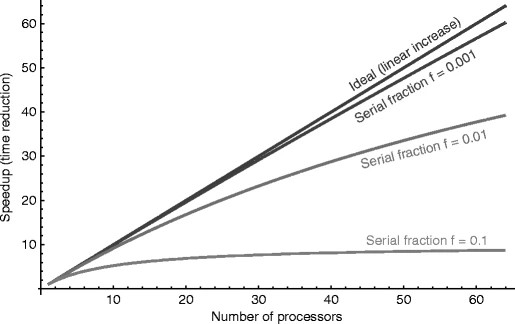
\includegraphics[width=0.7\textwidth]{img/amdahl.jpg}
    \caption{Factor de aceleración dependiendo de la fracción secuencial, según la ley de Amdahl \cite{Gustafson2011}}
    \label{fig:amdahl}
\end{figure}

\vspace{10pt}
Es razonable esperar que parte de las tareas computacionales no puedan ser divididas en procesos paralelos, teniendo
que ser ejecutadas secuencialmente. Supongamos que existe un periodo durante el cual únicamente está siendo utilizado 
un procesador, por ejemplo, un periodo de inicialización en el cual se están generando las posteriores tareas 
paralelas. A partir de esta asunción, lo ideal es que el resto de tareas sean realizadas por todos los procesadores 
disponibles trabajando simultáneamente. Si denotamos por $f$ a la fracción de la computación no paralelizable y $t_s$ 
al tiempo de ejecución del algoritmo secuencial, tenemos que el factor de aceleración es:
\begin{equation}\label{eq:ley-amdahl}
    S(p)=\frac{t_s}{f\cdot t_s+\displaystyle\frac{(1-f)t_s}{p}}=\frac{p}{1+(p-1)f}
\end{equation}
Esta ecuación es conocida como \textit{\textbf{ley de Amdahl}} \cite{wilkinson_allen_2005}. Esta ley nos hace inferir 
que el factor más importante a la hora de considerar la concurrencia es qué fracción de la computación es  
paralelizable, ya que, aún teniendo un número infinito de procesadores, la ganancia obtenida máxima será
\begin{equation}
    \lim_{p\to\infty} S(p)=\lim_{p\to\infty} \frac{p}{1+(p-1)f}=\frac{1}{f}
\end{equation}
Podemos ver este comportamiento de manera gráfica en la figura \ref{fig:amdahl}. Es importante notar que esta ecuación
es únicamente útil cuando la cantidad de tareas computacionales es fija.

% -------------------------------------------------------------------------------------------------------------------
\section{Escalabilidad}

No siempre un aumento de los procesadores tiene por qué implicar una mejora proporcional, como hemos visto a través de
la ley de Amdahl. Uno de los factores importantes a la hora de utilizar programas concurrentes es la escalabilidad.

\vspace{10pt}
Este término es, sin embargo, impreciso. Suele utilizarse para indicar en el diseño \textit{hardware} si un sistema,
al aumentar su tamaño, aumenta también su rendimiento. La escalabilidad también se utiliza para indicar si un algoritmo
paralelo, al aumentar el número de datos de entrada o trabajo computacional no aumenta de forma desproporcionada el
aumento de etapas de computación. Cuando se utiliza en este sentido, se le denomina 
\textbf{\textit{escalabilidad algorítmica}} \cite{wilkinson_allen_2005}. 

\vspace{10pt}
Para estudiar la escalabilidad de los algoritmos concurrentes, la ley de Amdahl no proporciona la información 
suficiente, por lo que es necesario utilizar otras medidas.

% -------------------------------------------------------------------------------------------------------------------
\subsubsection*{Ley de Gustafson}

El primer supuesto de la ley de Amdahl es la suposición de que la cantidad de trabajo computacional es fija. Esta
suposición es útil, puesto que evita definir el trabajo computacional, pero no tiene en cuenta que se puede buscar una
mejora computacional en lugar de una mejora temporal mediante la paralelización \cite{Gustafson2011}. 

\vspace{10pt}
En la práctica, la paralelización suele utilizarse para realizar tareas de computación mucho más grandes para que 
mantengan un tiempo de ejecución razonable, para lo cual necesitamos una medida que tenga en cuenta este factor, y que 
nos dará alguna medida de la escalabilidad algorítmica de los modelos utilizados. Por tanto, es válido asumir que el 
tiempo de ejecución del algoritmo es fijo, siendo la cantidad de trabajo computacional o tamaño de los datos de entrada 
la que varía entre la versión secuencial y la paralela. Utilizando este supuesto, el factor de aceleración será 
numéricamente distinto a los calculados anteriormente, y se le llama \textbf{\textit{factor de aceleración escalado}}, 
y fue formulado por Gustafson en 1988. En esta ecuación, es el tiempo de ejecución paralelo el que es constante, en 
lugar del secuencial \cite{wilkinson_allen_2005}. La ecuación, llamada usualmente \textbf{\textit{ley de Gustafson}}, 
tiene la forma
\begin{equation}
    S_s(p)=p+(1-p)f\cdot t_s=p-f(p-1)
\end{equation}

% -------------------------------------------------------------------------------------------------------------------
\subsubsection*{Paralelismo parcial}

No siempre un algoritmo puede paralelizar todas sus tareas de forma que se utilice el total de los procesadores 
disponibles, sino que puede haber diferentes grados de paralelización para sus diferentes tareas, como por ejemplo, los
algoritmos que utilizan técnicas como ``divide y vencerás'' \cite{SUN199327}. El modelo de Amdahl
no contempla este tipo de situaciones. Una ecuación más realista y detallada en la cual el paralelismo puede variar 
entre $1$ y $n$ procesadores es:
\begin{equation}
    S(n)=\frac{1}{f_1+\displaystyle\frac{f_2}2+\displaystyle\frac{f_3}3+\cdots+\displaystyle\frac{f_n}n}
\end{equation}
donde $f_i$ es la fracción del algoritmo que puede ser ejecutada por $i$ procesadores en paralelo, y $f_1+\cdots+f_n=1$
\cite{Gustafson2011}.

% -------------------------------------------------------------------------------------------------------------------
\subsubsection*{Comunicación entre procesos}

\vspace{10pt}
Debido al momento histórico de la formulación de la ley por Gene Amdahl, 1967, el coste de comunicación entre los
procesadores se estimó como insignificante. Esto fue así debido a que en ese momento la computación de los algoritmos
era magnitudes superiores en cuanto a tiempo que la comunicación entre los procesadores. La velocidad de computación
de los procesadores modernos es mucho mayor que la velocidad de comunicación de datos entre los mismos
\cite{Gustafson2011}.

\vspace{10pt}
Si denominamos $t_{\text{cm}}$ al tiempo de ejecución gastado en la comunicación entre los diferentes procesadores
y $t_{\text{cp}}$, podemos establecer una nueva medida, a la que llamaremos 
\textbf{\textit{ratio computación/comunicación}}, calculado como:
\begin{equation}
    R_{cc}=\frac{t_{\text{cp}}}{t_{\text{cm}}}
\end{equation}
Supongamos que disponemos de $p$ procesadores y $n$ elementos de datos para un algoritmo. El ratio nos permite conocer
el potencial de escalabilidad del algoritmo. Supongamos, por ejemplo, que para un valor $p$, tenemos que nuestro
algoritmo requiere $c_1n$ computaciones y $c_2n^2$ comunicaciones. 

\vspace{10pt}
Utilizando el ratio computación/comunicación, podemos ver que la paralelización no mejora sustancialmente el tiempo de 
ejecución del programa conforme va aumentando el número de elementos de datos, puesto que:
\begin{equation}
    R_{cc}=\frac{c_1n}{c_2n^2}=\frac{c_1}{c_2n}\Rightarrow\lim_{n\to\infty} R_{cc}=0
\end{equation}
Normalmente, vamos a preferir aquellas soluciones que maximicen el ratio computación/comunicación, es decir, aquellos
que transformen $R_{cc}$ es una función creciente respecto a $n$. Es importante notar que para obtener esta medida,
es necesario ejecutar el programa primero, calculando después el ratio \cite{wilkinson_allen_2005}.

% -------------------------------------------------------------------------------------------------------------------
\section{Clústeres}

Una de las formas de obtener un multiprocesador es el uso de \textbf{\textit{clústeres}}, que no es más que duplicar
unidades procesamiento y combinarlas. Los clústeres se conciben como sistemas de computación paralela constituidos por
\textbf{\textit{nodos}} interconectados, compuestos por procesadores, memorias, buses, \dots; que cooperan entre sí.
Los nodos se comunican entre sí mediante el paso de mensajes. Dependiendo de los componentes de la arquitectura, se 
pueden definir distintos tipos de clústeres \cite{czech_2017}.

\begin{figure}[htbp!]
    \centering
    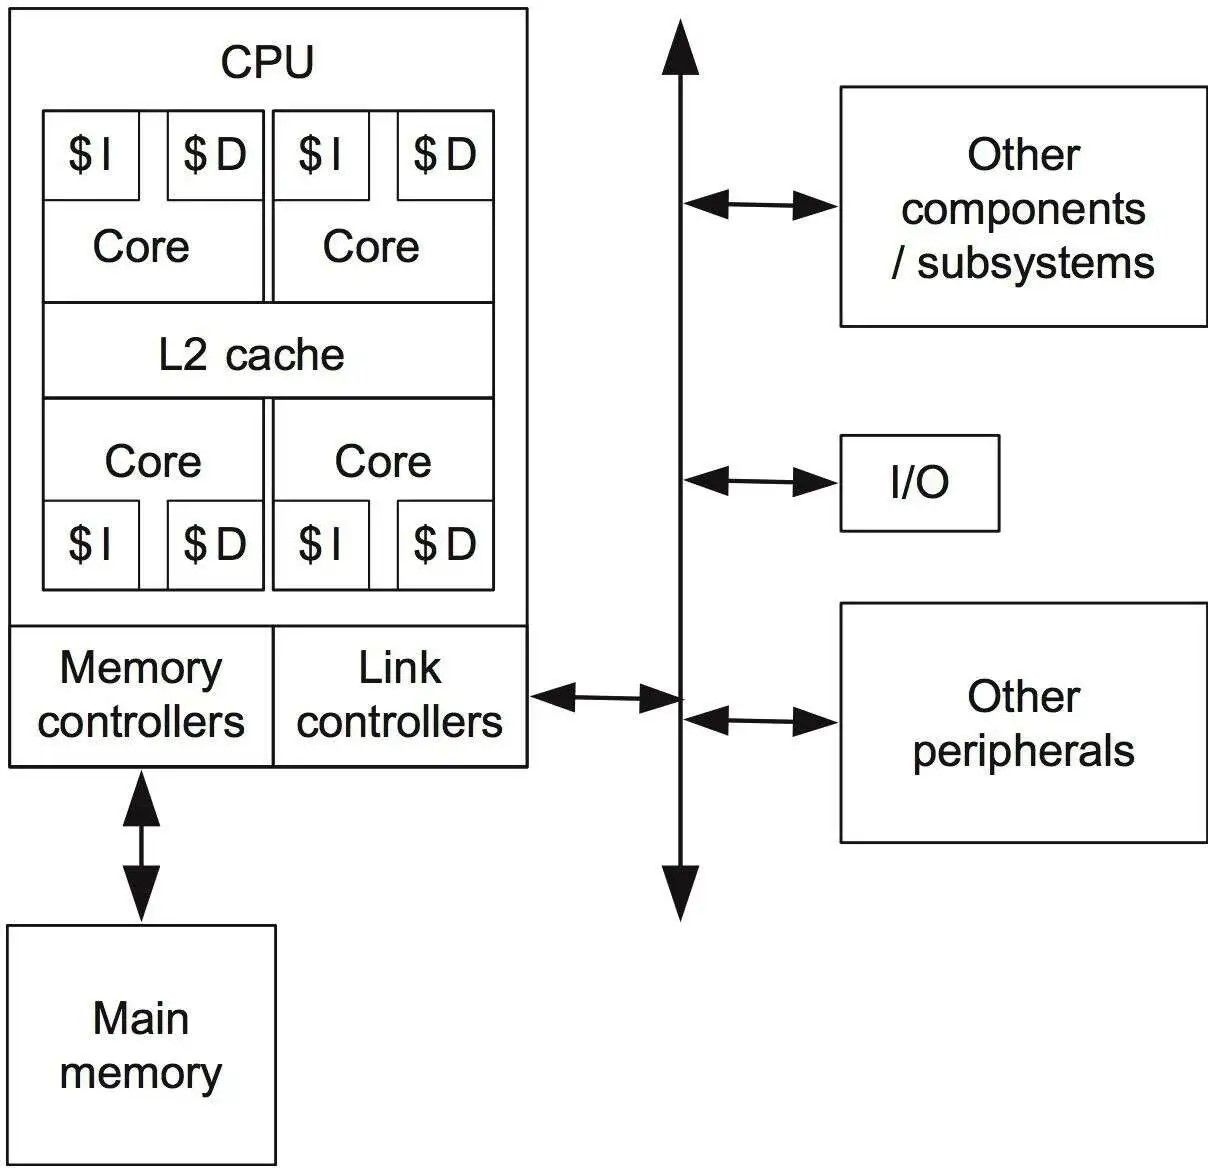
\includegraphics[width=0.6\textwidth]{img/MCP.jpg}
    \caption{Arquitectura de clúster de procesador con cuatro núcleos \cite{mcp}.}
    \label{fig:mcp}
\end{figure}

% -------------------------------------------------------------------------------------------------------------------
\subsection{Procesador multinúcleo}

La estructura de este tipo de clústeres se basa en la unión de varias unidades de procesamiento separadas, denominadas
núcleos, en un único chip. De esta manera, se puede construir una máquina capaz de ejecutar diferentes tareas de
computación en diferentes partes de la memoria. La memoria en este clúster es común para todos nodos (núcleos), así 
como el resto de componentes de la máquina. La mayoría de computadores actualmente presentan esta arquitectura. Un 
esquema de este tipo de clúster es el de la figura \ref{fig:mcp}.

\vspace{10pt}
Debido a que este tipo de clústeres la mayor parte de la computación y comunicación se realiza sobre memoria 
compartida, son más adecuados para implementar algoritmos de granularidad fina y con referencias a datos diversas, es
decir, datos locales y no locales \cite{czech_2017}.

% -------------------------------------------------------------------------------------------------------------------
\subsection{Clúster de computadores}

Un clúster de computadores se construye conectando mediante una red una cierta cantidad de computadores, conformando
cada uno de ellos un nodo. Si los computadores son idénticos en términos de arquitectura, hardware y software, se dice
que el clúster es \textit{homogéneo} \cite{czech_2017}. Es posible combinar varias arquitecturas, es decir, podemos
tener un clúster de computadores conformado por máquinas con procesadores multinúcleo.

\vspace{10pt}
El uso de una red de computadores tiene ventajas sobre el uso de sistemas multiprocesadores específicos. Las ventajas
clave son:
\begin{enumerate}
    \item Los PCs o estaciones de trabajo de grandes prestaciones son fáciles de adquirir a un bajo coste.
    \item Los procesadores pueden ser sustituidos conforme otros con mejores prestaciones van apareciendo, y el clúster 
    puede cambiar de tamaño fácilmente, aumentando o disminuyendo el número de máquinas.
    \item Es posible utilizar aplicaciones software existentes sobre el clúster.
\end{enumerate}
\begin{figure}[htbp!]
    \centering
    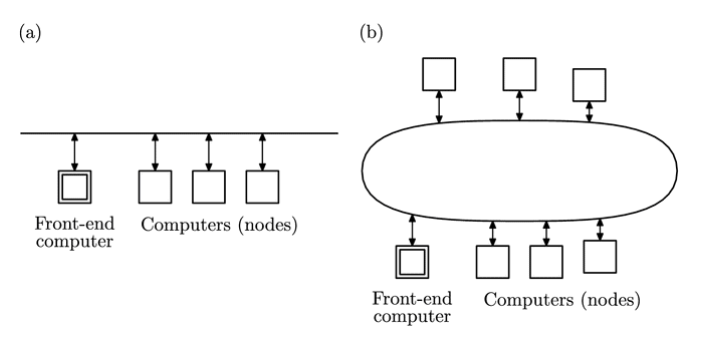
\includegraphics[width=0.8\textwidth]{img/cluster.png}
    \caption{Clúster de computadores: conectados mediante un único cable de red (a) o con una topología de anillo (b). En ambos casos, un nodo \textit{front-end} se encarga de la gestión del clúster \cite{czech_2017}.}
    \label{fig:cluster}
\end{figure}

\vspace{10pt}
El caso más común de clúster de computadores es la conexión mediante cables Ethernet de computadores mediante diversas
topologías de red, como se muestra en la figura \ref{fig:cluster}. El primero de ellos fue construido en 1994 en el 
Centro de Vuelo Espacial Goddard de la NASA, en el cual se conectaron los ordenadores personales de los ingenieros. 
Sus creadores lo denominaron Beowulf a raíz del héroe legendario medieval. Podemos decir que este tipo de clústeres 
son \textit{centralizados}, mientras que los denominados \textit{descentralizados} suelen estar conformados por nodos 
separados físicamente y conectados mediante Internet, donde cada nodo puede ser reconfigurado, encendido o apagado en 
cualquier momento \cite{czech_2017}.

% -------------------------------------------------------------------------------------------------------------------
\subsection{Memoria compartida distribuida}

Uno de los problemas que puede acarrear un clúster de computadores centralizado es la formación de un cuello de 
botella en el paso de información, ya que el acceso a la memoria y el paso de mensajes se realiza a través de un canal 
de red.  La \textbf{\textit{memoria compartida distribuida}} (DSM) es una posible solución a este problema. Esta 
arquitectura, apreciable en la figura \ref{fig:dsm}, ofrece un espacio de direcciones virtual compartido por todos los 
nodos de la red, evitando así la necesidad de paso de mensajes entre los distintos procesadores \cite{nitzberg_91}.

\begin{figure}[htbp!]
    \centering
    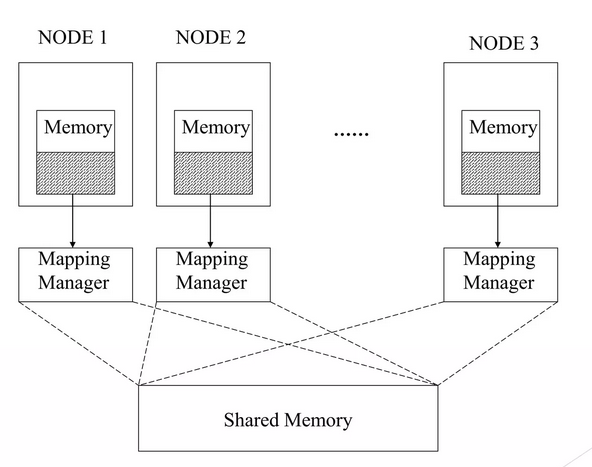
\includegraphics[width=0.6\textwidth]{img/dsm.png}
    \caption{Arquitectura de memoria compartida distribuida \cite{dsm}.}
    \label{fig:dsm}
\end{figure}

\vspace{10pt}
Las ventajas de esta arquitectura frente tanto a un clúster de computadores usual o a un multiprocesador con memoria 
compartida son las siguientes:
\begin{itemize}
    \item Suele resultar más natural programar algoritmos concurrentes utilizando memoria compartida en lugar de paso
    de mensajes explícito. En ocasiones, como puede ser estructuras que contengan punteros, puede llegar a ser incluso
    imposible.
    \item La mayoría de programas están escritos para ser ejecutados en multiprocesadores con memoria compartida 
    (procesadores multinúcleo). Los sistemas DSM permiten ejecutar ese tipo de programas.
    \item Algoritmos que requieran grandes cantidades de memoria pueden ser ejecutados sin problema en esta 
    arquitectura, ya que los procesadores tienen acceso a una gran cantidad de memoria compartida.
    \item El intercambio de datos a través de bloques de memoria es más eficiente que el paso de información a través
    de mensajes.
\end{itemize}
Uno de los problemas principales de esta arquitectura es la gestión de la heterogeneidad entre los distintos nodos de
la red. Al tener memoria compartida, puede suponer grandes costes computacionales la transformación de los datos si
los nodos tienen diferentes formas de representación de los mismos \cite{nitzberg_91}.

% -------------------------------------------------------------------------------------------------------------------
\section{Spark}

La herramienta utilizada para realizar la paralelización en este trabajo es Spark. Esta herramienta se puede utilizar
tanto en en clústeres de ordenadores como un en un clúster independiente, es decir, una sola máquina. Forma parte 
de la \textit{Apache Software Foundation}, una organización sin ánimo de lucro responsable de algunos de los proyectos 
de software libre más importantes. Basada en los RDDs, \textit{resilient distributed datasets}, descritos por Matei 
Zaharia y otros en la Universidad de California, Spark es la herramienta más utilizada para realizar tareas 
computacionales escalables y ciencia de datos \cite{spark}.

% -------------------------------------------------------------------------------------------------------------------
\subsection{RDDs}

Los RDDs, \textit{resilient distributed datasets} o \textbf{\textit{conjuntos de datos resilientes distribuidos}} en
castellano, son estructuras paralelas tolerantes a fallos que permiten la persistencia de resultados intermedios en
memoria, pudiendo manipularlos mediante un conjunto de operadores. Son especialmente útiles para aplicaciones en las
cuales se reutilizan cálculos intermedios a lo largo de múltiples computaciones, como pueden ser la mayoría de 
algoritmos de aprendizaje automático iterativos: regresión logística, $K$-medias, \dots \cite{rdds}

\vspace{10pt}
Formalmente, un RDD es una colección particionada de registros de sólo lectura. Pueden ser creados a partir de 
operaciones deterministas sobre datos en un almacenamiento estable o a partir de otros RDDs. A estas operaciones las
denominaremos \textit{transformaciones} para diferenciarlas del resto de operaciones. Ejemplos de estas 
transformaciones son el mapeo, los filtros y la unión.

\vspace{10pt}
El objetivo principal de los RDDs es definir una interfaz programática que sea capaz de proveer tolerancia a fallos de
forma eficiente. Las arquitecturas de memoria compartida distribuida ofrecen una interfaz basada en actualizaciones
de granularidad fina de estados mutables como por ejemplo, celdas de una tabla. La única manera de proveer tolerancia
a fallos es replicar los datos en otras máquinas o registrar las actualizaciones en los nodos \cite{rdds}. 

\vspace{10pt}
Ambos enfoques son costosos para cargas de trabajo con uso intensivo de datos, puesto que requieren copiar grandes 
cantidades de datos a través de la red del clúster, cuyo ancho de banda suele ser mucho menor que el de la RAM, 
incurriendo en una sobrecarga sustancial de almacenamiento \cite{rdds}.

\vspace{10pt}
A diferencia de esa arquitectura, los RDDs ofrecen una interfaz basada en operaciones de poca granularidad 
(transformaciones) que aplican la misma operación a muchos elementos de datos. Esto les permite tolerar fallos 
registrando las transformaciones utilizadas para construir el conjunto de datos, lo que llamaremos \textit{linaje}, en 
lugar de los datos reales. Si una partición de un RDD se pierde, el RDD tiene información suficiente sobre cómo se 
obtuvo de otros RDDs para volver a calcular sólo esa partición. De esta manera, los datos perdidos pueden recuperarse, 
a menudo con bastante rapidez, sin necesidad de una costosa replicación. Aunque inicialmente pueda parecer limitada una 
interfaz basada en transformaciones de poca granularidad, los RDDs son una buena solución para la mayoría de programas 
paralelos, porque estas aplicaciones realizan de forma natural la misma operación sobre múltitud de datos\cite{rdds}.

\vspace{10pt}
Un RDD no tiene por qué estar materializado en todo momento, más bien al contrario, puesto que contiene suficiente
información acerca de cómo fue construido a través de su linaje para computar sus particiones a partir de los datos
en el almacenamiento estable. En esencia, un programa no puede referenciar un RDD que no sea capaz de reconstruir 
después de un fallo \cite{rdds}.

% -------------------------------------------------------------------------------------------------------------------
\subsubsection*{Ventajas}

Para comprender los beneficios de los RDDs como arquitectura de memoria distribuida, vamos a compararlos con la 
arquitectura de memoria compartida distribuida, cuyo resumen se puede ver en la tabla \ref{tab:rdds}. Para entender la
comparativa, es importante notar que, en los sistemas DSM, las aplicaciones pueden leer y escribir en regiones 
arbitrarias de la memoria global compartida \cite{rdds}.

\vspace{10pt}
La diferencia principal entre las arquitecturas es que los RDDs solamente pueden crearse (lo que viene a ser 
``escribirse'', al ser inmutables) mediante transformaciones, que son de poca granularidad, mientras que la DSM permite
lecturas y escrituras a cualquier región de la memoria. Esto restringe a los RDDs a aplicaciones que realizan 
escrituras en masa, en beneficio de una tolerancia a fallos muy eficiente. En particular, los RDDs no generan 
sobrecargas al no necesitar puntos de control, puesto que pueden reconstruirse a partir de su linaje. Además, sólo las
particiones perdidas de un RDD necesitan recomputarse en caso de fallo, y pueden reconstruirse de forma paralela en
distintos nodos sin tener que hacer una vuelta atrás del programa \cite{rdds}.

\begin{table}[htbp!]
\begin{tabular}{|p{0.25\textwidth}|p{0.32\textwidth}|p{0.32\textwidth}|}
\hline
\multicolumn{1}{|c|}{\textbf{Característica}} & \multicolumn{1}{c|}{\textbf{RDDs}} & \multicolumn{1}{c|}{\textbf{DSM}} \\ \hline
\textit{Lecturas} & Escala completa de granularidad & Granularidad fina \\ \hline
\textit{Escrituras} & Poca granularidad & Granularidad fina \\ \hline
\textit{Consistencia} & Trivial (inmutables) & Responsabilidad de la aplicación o \textit{runtime} \\ \hline
\textit{Recuperación de fallos} & Granularidad fina y poca sobrecarga utilizando el linaje & Requiere puntos de control y vueltas atrás del programa \\ \hline
\textit{Mitigación de rezagados} & Posible utilizando tareas de respaldo & Difícil \\ \hline
\textit{Reparto de tareas} & Automática basada en la localidad de datos & Responsabilidad de la aplicación \\ \hline
\textit{Comportamiento ante sobrecarga} & Similar a otros sistemas de flujos de datos & Bajo rendimiento \\ \hline
\end{tabular}
\caption{Comparativa entre RDDs y memoria compartida distribuida \cite{rdds}.}
\label{tab:rdds}
\end{table}

\vspace{10pt}
Otra de las ventajas que proporcionan los RDDs es su inmutabilidad. Gracias a ella, son capaces de mitigar los nodos
lentos o rezagados lanzando copias de respaldo de las tareas lentas. Estas tareas de respaldo serían muy difíciles de
implementar en DSM, puesto que ambas copias de la tarea accederían a las mismas direcciones de memoria, interfiriendo
en las actualizaciones de cada una \cite{rdds}.

\vspace{10pt}
Finalmente, en operaciones masivas sobre RDDs, un \textit{runtime} reparte y programa las tareas basándose en la 
localidad de los datos para mejorar el rendimiento. Además, para operaciones masivas que sobrecargan el sistema en 
cuanto a memoria, los RDDs se degradan con elegancia siempre y cuando sólo se utilicen en operaciones de escaneo. Las 
particiones que no caben en la memoria se pueden almacenar en el disco y brindan un rendimiento similar al resto de 
sistemas de datos en paralelo \cite{rdds}.

% -------------------------------------------------------------------------------------------------------------------
\subsection{Interfaz}

Spark expone los RDDs mediante una API integrada en el lenguaje Scala, aunque existen librerías actualmente de Spark en
muchos otros lenguajes, como Python. Cada conjunto de datos se representa en esta API como un objeto, y las 
transformaciones se invocan como métodos sobre esos objetos.

\vspace{10pt}
Para programar utilizando RDDs, se comienza definiendo uno o más RDDs mediante transformaciones sobre datos en un
almacenamiento estable. Después se pueden utilizar estos objetos en \textit{acciones}, operaciones que devuelven un
valor a la aplicación o exportan datos a un sistema de almacenamiento. Ejemplos de estas acciones son:
\begin{itemize}
    \item \textit{count}: Devuelve el número de elementos del conjunto de datos.
    \item \textit{collect}: Devuelve los elementos del conjunto de datos explícitamente.
    \item \textit{save}: Guarda los datos en el sistema de almacenamiento.
\end{itemize}
Spark realiza la computación de los RDDs de forma diferida la primera vez que se utilizan en una acción, pudiendo de
esta manera encadenar transformaciones \cite{rdds}.

\vspace{10pt}
Además, se puede llamar a un método de persistencia para indicar qué RDDs se desea reutilizar en operaciones futuras.
Spark mantiene estos objetos en memoria por defecto, pero puede volcarlos al almacenamiento en disco si no queda
suficiente espacio en RAM. También implementa otras estrategias de persistencia, como el almacenamiento del RDD 
únicamente en disco o replicando un RDD en varias máquinas mediante parámetros del método \textit{persist} \cite{rdds}.

\vspace{10pt}
Para utilizar Spark, un programador debe escribir un \textit{programa controlador} que se conecta a un clúster de
\textit{trabajadores}. Este controlador define los RDDs e invoca las acciones sobre ellos. El código de Spark en el
controlador es también el que lleva el linaje de los RDDs. Los trabajadores son procesos de larga duración que 
almacenan las particiones del RDD en la RAM a lo largo de las operaciones \cite{rdds}. El algoritmo de aprendizaje
distribuido implementado en la herramienta sería en este caso el programa controlador, y hablaremos de él en el 
siguiente capítulo.

\endinput
%--------------------------------------------------------------------
% FIN DEL CAPÍTULO. 
%--------------------------------------------------------------------

% !TeX root = ../tfg.tex
% !TeX encoding = utf8

\chapter{Optimización por enjambre de partículas}\label{chap:pso}

A lo largo de los siglos, la naturaleza ha sido siempre una fuente de inspiración para la humanidad. La inteligencia
de enjambre, una rama de la inteligencia artificial, intenta emular los comportamientos de inteligencia colectiva de
enjambres de la naturaleza. Normalmente, un enjambre se define como un gran número de agentes sencillos y homogéneos
que interactúan localmente con su entorno, así como con sí mismos, con un control descentralizado del que emerge un
comportamiento global \cite{gad_2022}.

\vspace{10pt}
El algoritmo de \textbf{\textit{optimización por enjambre de partículas}} o \textbf{\textit{PSO}} 
(\textit{particle swarm optimization}) es uno de los modelos de inteligencia de enjambre más populares. El PSO es
un algoritmo estocástico propuesto originalmente en la década de 1990, inspirado por los comportamientos sociales de
animales como las bandadas de pájaros o los bancos de peces. En este algoritmo, cada solución potencial de un problema
se representa como una partícula con una cierta velocidad que vuela sobre el espacio de definición del problema, como
si de un pájaro se tratara. Cada partícula combina después algún aspecto del registro de su mejor ubicación y la actual
con algunas otras del enjambre para determinar su próximo movimiento. El enjambre en su conjunto, como por ejemplo un
banco de peces en búsqueda de alimento, se acerca gradualmente al óptimo de la función objetivo \cite{gad_2022}.

\vspace{10pt}
En este capítulo vamos a estudiar este algoritmo para su uso en redes neuronales prealimentadas de una capa. En primer
lugar, hablaremos de las características y estructura general del algoritmo, para luego hablar del implementado en la
herramienta: el \textbf{\textit{algoritmo de optimización por enjambre de partículas asíncrono distribuido}} o 
\textbf{\textit{DAPSO}} (\textit{distributed asynchronous PSO}).

% -------------------------------------------------------------------------------------------------------------------
\section{Descripción del algoritmo}

% -------------------------------------------------------------------------------------------------------------------
\subsection{Definiciones}

Para simplificar las definiciones, vamos a suponer que el problema que estamos intentando resolver es el de búsqueda
de un mínimo, que se corresponde justamente con el proceso de entrenamiento de una red, en el cual intentamos minimizar
la función de costo. Dada una función $f$ o función objetivo, denominada \textit{fitness}, definida en un espacio de 
$D$ dimensiones, al que llamaremos \textit{espacio de búsqueda}, el objetivo del algoritmo es encontrar el punto de ese
espacio en el cual la función alcanza su mínimo \cite{clerc_12}.

\vspace{10pt}
Para el caso de uso de la herramienta, tenemos que $f$ será o el error cuadrático medio de la red o la 
exactitud (\textit{accuracy}) de la red (en cuyo caso utilizamos $1-\text{exactitud}$ para transformar el 
problema a uno de minimización), y por tanto el valor de la $\textit{fitness}$ dependerá también de los 
ejemplos utilizados. Definimos ahora el espacio de búsqueda como:

\begin{definicion}[Espacio de búsqueda]Denominamos \textit{espacio de búsqueda} ($E$) al hiperparalelepípedo 
definido como el producto euclídeo de $D$ intervalos reales
\begin{equation}
    E=\bigotimes_{d=1}^D[\min(d),\max(d)]
\end{equation}
donde $\min(d)$ (resp. $\max(d)$) es el valor mínimo (resp. máximo) que puede darse en esa componente \cite{clerc_12}.
\end{definicion}

En el caso de uso de la herramienta, el espacio de búsqueda será el producto euclídeo de los dominios de los pesos de
la red, siendo $D$ entonces el número total de pesos de la red neuronal.

\vspace{10pt}
Un \textbf{\textit{enjambre}} será un conjunto ordenado de $S$ partículas, numeradas desde $0$ a $S-1$, donde cada 
partícula se define como:

\begin{definicion}[Partícula] Una partícula es una tripla de vectores $D$ dimensionales $\big(x(t),v(t),p(t)\big)$, 
con 
$x(t),p(t),g(t)\in E$, donde:
\begin{enumerate}[(a)]
    \item $x(t)$ es la posición de la partícula en el valor de tiempo $t$.
    \item $v(t)$ es la velocidad de la partícula en el valor de tiempo $t$.
    \item $p(t)$ es la mejor posición local de la partícula hasta el momento $t$.
\end{enumerate}
\end{definicion}

Se definen $p_i(t)$ para cada partícula del enjambre y $g(t)$, la mejor posición global del enjambre, de la siguiente 
manera:
\begin{align}
    p_i(t)&=\min_{k=1,\dots,t}\Big(f\big(x_i(k)\big)\Big) \\
    g(t)&=\min_{\substack{j=0,\dots,S-1 \\ k=1,\dots,t}}\Big(f\big(p_j(k)\big)\Big)
\end{align}
Donde $f$ es la función \textit{fitness} que queremos minimizar \cite{gad_2022}.

% -------------------------------------------------------------------------------------------------------------------
\subsection{Inicialización}

El primer paso del algoritmo PSO es la inicialización. Para ello, primero debemos definir el número de partículas para
el algoritmo. Las primeras definiciones del algoritmo proponían un valor fijo dependiendo de la dimensión del espacio
de búsqueda, mediante esta fórmula:
\begin{equation}\label{eq:pso-init}
    S=10+2\sqrt{D}
\end{equation}
Sin embargo, este número suele estar alejado del valor óptimo. El valor inicial sugerido es 40 \cite{clerc_12}. 

\vspace{10pt}
Una vez elegido el número de partículas, el algoritmo inicializa a valores ``aleatorios'' cada partícula. Denotamos 
este paso con el momento temporal $0$. Para cada partícula $i$ del enjambre, se inicializan sus valores y la mejor
posición global del enjambre de la siguiente manera:
\begin{align}\label{eq:pso-part}
    &\text{Para cada }j=1,\dots,D\quad x_{ij}(0)=U(m_1,m_2) \\
    &\text{Para cada }j=1,\dots,D\quad v_{ij}(0)=U(m_1-x_{ij}(0),m_2-x_{ij}(0)) \\
    &p_i(0)=x_i(0) \\
    &g(0)=\min_{i=0,\dots,S-1}\Big(f\big(p_j(0)\big)\Big)
\end{align}
donde $U$ denota la distribución uniforme y $m_1$, $m_2$ pueden ser o parámetros dados simbolizando los valores límite
del espacio de búsqueda o $\min(d)$ y $\max(d)$ respectivamente \cite{clerc_12}.

% -------------------------------------------------------------------------------------------------------------------
\subsection{Iteraciones}

Una vez inicializadas las partículas, se realiza un cierto número de iteraciones, que puede ser un valor prefijado o
una condición de parada. Usualmente esta condición suele ser un valor umbral para la función \textit{fitness}, o un
número máximo de iteraciones en la cual no haya una mejora (reducción en nuestro caso) de esa misma función 
\cite{clerc_12}. En cada una de esas iteraciones, que se corresponden con un valor entero de $t$, se realizan los 
siguientes pasos:
\begin{enumerate}
    \item Se calcula, para cada partícula, una nueva velocidad, utilizando la siguiente fórmula:
    \begin{equation}\label{eq:pso-vel}
        v_i(t+1)=w\cdot v_i(t) + U(0,c_1)(p_i(t)-x_i(t))+U(0,c_2)(g(t)-x_i(t))
    \end{equation}
    donde $w$ es el peso de inercia de la velocidad \cite{gad_2022}, que puede ser un valor prefijado o 
    $\frac{1}{2\ln{2}}$ \cite{clerc_12}, y $c_1$, $c_2$ son parámetros fijos o, alternativamente, $\frac{1}{2}+\ln{2}$
    \cite{clerc_12}. Normalmente, se define un intervalo máximo para la velocidad de las partículas para intentar 
    prevenir que las partículas se alejen del espacio de búsqueda, forzando una cierta velocidad máxima por etapa con 
    la intención de que éstas peinen el espacio de búsqueda completo \cite{gad_2022}.
    \item Para cada partícula del enjambre, se actualiza su posición:
    \begin{equation}\label{eq:pso-pos}
        x_i(t+1)=x_i(t)+v_i(t+1)
    \end{equation}
    De la misma manera que para la velocidad, se pueden establecer valores umbrales para la posición, restringiendo
    de esta manera el movimiento de las partículas al espacio de búsqueda. Estos valores son los mismos que los $m_1$
    y $m_2$ definidos en la inicialización.
    \item Comprobamos, en cada partícula, si la posición actual es mejor que la mejor posición global. En caso
    afirmativo, actualizamos ese valor.
    \item Una vez calculados todos los valores anteriores, modificamos el valor de la mejor posición global en caso de
    ser necesario.
\end{enumerate}

% -------------------------------------------------------------------------------------------------------------------
\subsection{Pseudocódigo}

Sea $f:\mathbb{R}^n\to\mathbb{R}$ la función objetivo que queremos minimizar. El algoritmo toma como valores de 
entrada el número de partículas $S$, los valores umbrales de posición y velocidad $p_{\max}$ y $v_{\max}$, los valores
de las constantes y el peso de inercia $w$, $c_1$ y $c_2$ y un número de iteraciones $T$. A partir de estos valores,
el mínimo global $g$ se calcula como sigue en el algoritmo \ref{alg:pso}.

\begin{algorithm}[htb!]
\caption{Pseudocódigo del PSO}\label{alg:pso}
\begin{algorithmic}[1]
\Require $S$, $p_{\max}$, $v_{\max}$, $w$, $c_1$, $c_2$, $T$
\Ensure $g$
\For{$i=0,\dots,S-1$} 
    \State Inicializamos partícula según \eqref{eq:pso-part} 
\EndFor
\State $g\gets (\infty,\dots,\infty)$
\State $t\gets 1$
\While{$t\leq T$}
    \For{$i=0,\dots,S-1$} 
    \State Actualizamos velocidad según \eqref{eq:pso-vel}
    \If{$v_i>v_{\max}$}
        \State $v_i\gets v_{\max}$
    \ElsIf{$v_i<-v_{\max}$}
        \State $v_i\gets -v_{\max}$
    \EndIf
    \State Actualizamos posición según \eqref{eq:pso-pos}
    \If{$x_i>p_{\max}$}
        \State $x_i\gets p_{\max}$
    \ElsIf{$x_i<-p_{\max}$}
        \State $x_i\gets -p_{\max}$
    \EndIf
    \If{$f(x_i)<f(p_i)$}
        \State $p_i\gets x_i$
    \EndIf
    \If{$f(x_i)<f(g)$}
        \State $g\gets x_i$
    \EndIf
    \EndFor
    \State $t\gets t+1$
\EndWhile
\\\Return $g$
\end{algorithmic}
\end{algorithm}

% -------------------------------------------------------------------------------------------------------------------
\section{Versión distribuida: DAPSO}

Una de las grandes ventajas de la optimización por enjambre de partículas es su facilidad para paralelizarse, puesto
que como hemos visto, cada partícula se actualiza por separado, únicamente utilizando la información del resto para
actualizar el valor de la mejor posición global. Esta ventaja, junto con uno de los problemas principales del algoritmo, la gran carga computacional que conlleva la gran cantidad de evaluaciones de la función objetivo, lo hace
un muy buen candidato para la paralelización. Vamos ahora a comentar la versión del PSO que ha sido implementada 
para la herramienta, distribuida y asíncrona, que utiliza los RDDs de Spark para paralelizar la actualización de
posiciones y velocidades de las partículas. Al utilizar Spark y sus transformaciones de poca granularidad, el 
enjambre se divide en múltiples subenjambres que se evalúan en paralelo \cite{dapso}.

\begin{figure}[th!]
    \selectcolormodel{gray}
    \centering
        \begin{tikzpicture}[node distance=1.5cm]
            \node (start) [startstop] {\footnotesize Iniciar maestro};
            \node (init_1) [process, below of=start] {\footnotesize Inicializar el enjambre y el estado};
            \node (init_2) [process, below of=init_1] {\footnotesize Cargar las partículas iniciales en la cola};
            \node (dist) [process, below of=init_2, yshift=-0.1cm] {\footnotesize Distribuir las partículas de la cola a los nodos esclavos};
            \node (wait) [process, below of=dist, yshift=-0.3cm] {\footnotesize Esperar a cada partícula evaluada de los nodos esclavos};
            \node (update_1) [process, below of=wait, yshift=-0.6cm] {\footnotesize Actualizar la mejor posición global basándose en cada partícula};
            \node (update_2) [process, below of=update_1, yshift=-0.6cm] {\footnotesize Actualizar la posición y velocidad de cada partícula};
            \node (dec) [decision, right of=update_2, xshift=3cm] {\footnotesize Se cumple la condición de parada};
            \node (nop) [process, right of=dist, xshift=3cm] {\footnotesize Cargar la partícula de vuelta};
            \node (yep) [process, below of=update_2, yshift=-0.5cm] {\footnotesize Devolver la mejor posición global};
            \node (end) [startstop, below of=yep] {\footnotesize Finalizar maestro};

            \draw [arrow] (start) -- (init_1);
            \draw [arrow] (init_1) -- (init_2);
            \draw [arrow] (init_2) -- (dist);
            \draw [arrow] (dist) -- (wait);
            \draw [arrow] (wait) -- (update_1);
            \draw [arrow] (update_1) -- (update_2);
            \draw [arrow] (update_2) -- (dec);
            \draw [arrow] (dec) -- node[anchor=east] {no} (nop);
            \draw [arrow] (nop) -- (dist);
            \draw [arrow] (dec) |- node[anchor=north] {sí} (yep);
            \draw [arrow] (yep) -- (end);
        \end{tikzpicture}
    \caption{Diagrama de flujo del nodo maestro con subenjambres de tamaño $1$.}
    \label{fig:dapso_master}
\end{figure}

\vspace{10pt}
En el algoritmo DAPSO, las partículas se actualizan en función del estado actual de todo el enjambre, es decir, 
tanto la posición como la velocidad de cada partícula se modifican tan pronto como se evalúa la función de 
\textit{fitness}, considerando de esta manera la mejor posición global encontrada hasta ese momento. Esto crea una 
independencia total entre las partículas, que se mueven a su siguiente posición con la información de la que 
disponen en el momento de la evaluación
\cite{dapso}.

\begin{figure}[th!]
    \selectcolormodel{gray}
    \centering
        \begin{tikzpicture}[node distance=2cm]
            \node (start) [startstop] {\footnotesize Iniciar trabajador};
            \node (wait) [process, below of=start] {\footnotesize Esperar un subenjambre del maestro};
            \node (eval_1) [process, below of=wait, yshift=-0.6cm] {\footnotesize Evaluar \textit{fitness} y mejor posición local de cada partícula};
            \node (send) [process, below of=eval_1, yshift=-0.4cm] {\footnotesize Enviar subenjambre de vuelta al maestro};
            \node (dec) [decision, right of=send, xshift=3cm] {\footnotesize Nodo maestro ha finzalizado};
            \node (end) [startstop, below of=dec,  yshift=-1cm] {\footnotesize Finalizar trabajador};

            \draw [arrow] (start) -- (wait);
            \draw [arrow] (wait) -- (eval_1);
            \draw [arrow] (eval_1) -- (send);
            \draw [arrow] (send) -- (dec);
            \draw [arrow] (dec) |- node[anchor=west] {no} (wait);
            \draw [arrow] (dec) -- node[anchor=east] {sí} (end);
        \end{tikzpicture}
    \caption{Diagrama de flujo de un nodo trabajador.}
    \label{fig:dapso_slave}
\end{figure}

\vspace{10pt}
El algoritmo distribuido sigue el paradigma maestro-trabajador: un nodo maestro es el responsable de coordinar al 
resto, los nodos trabajadores, que se encargan de realizar las computaciones enviadas por el maestro. Cada 
partícula del enjambre se mueve y evalúa la \textit{fitness} de manera autónoma \cite{dapso}. En las figuras 
\ref{fig:dapso_master} y \ref{fig:dapso_slave} pueden verse las diferentes tareas que ejecutan cada uno de estos 
nodos.

\vspace{10pt}
Por razones de eficiencia, el algoritmo utiliza una abstracción llamada \textbf{\textit{SuperRDD}}, compuesta por un
conjunto de partículas que son dependientes entre si y son ejecutadas en el clúster como un único subenjambre. Esto
significa que en lugar de enviar al clúster cada partícula de forma independiente, se agrupan en subenjambres de 
tamaño variable entre $1$ y $S$, donde $S$ es el número de partículas. Cuanto más grande el tamaño del subenjambre,
menor el grado de asincronía del algoritmo, ya que más partículas pasan a ser dependientes unas de otras. Sin 
embargo, esta modificación mejora la eficiencia del algoritmo, puesto que elimina parte de la sobrecarga 
computacional de la comunicación entre los nodos en sacrificio de asíncronía, ya que el nodo maestro detiene el
cálculo global esperando resultados parciales \cite{dapso}.

\vspace{10pt}
En el contexto de Spark, el SuperRDD consiste en la agrupación de varias partículas en un único RDD que luego es
evaluado por el clúster. De esta manera, y conforme aumenta el número de partículas del RDD, menos trabajos de Spark
tienen que programarse, disminuyendo la sobrecarga de comunicación, con el coste de que las partículas deben esperar
a que el resto del RDD sea evaluado por el nodo \cite{dapso}.

\vspace{10pt}
En cuanto a la implementación en Scala y Spark, dos conceptos son clave para el correcto funcionamiento: un 
acumulador, que reciba los datos de las partículas evaluadas (o los SuperRDDs) de nodos trabajadores y una manera de
distribuir esas partículas a los nodos trabajadores. 

\vspace{10pt}
La implementación del acumulador se compone de un canal de comunicación (clase \texttt{Channel}) que es capaz de 
almacenar listas de números. Hemos denominado \texttt{fuch} a este canal acumulador. Los nodos trabajadores, 
conforme evalúan las partículas, envían a ese canal una lista que contiene la posición de la partícula, su 
velocidad, el valor evaluado de \textit{fitness}, \dots El nodo maestro luego lee los elementos de ese canal para 
actualizar los valores de las partículas.

\begin{figure}[ht!]
    \centering
    \StartLineAt{43}
    \begin{lstlisting}[language=Scala, caption={}]
val srch = new Channel[BatchPSO]()
val fuch = new Channel[ListBuffer[Array[Double]]]()
    \end{lstlisting}
    \caption{Declaración de los canales en \texttt{DAPSO.scala}.}
    \label{fig:dapso-impl-1}
\end{figure}
\begin{figure}[ht!]
    \centering
    \StartLineAt{76}
    \begin{lstlisting}[language=Scala]
val iters = nIters * nParticles / batchSize
for (i <- 0 until iters) {
// Read from the Fitness writing channel
var data = fuch.read

var pos: Array[Double] = new Array[Double](0)
var velocity: Array[Double] = new Array[Double](0)
var bestGlobalPos: Array[Double] = new Array[Double](0)
var fit: Double = 0

// PSO
for (posVel <- data) {
  pos = posVel.slice(0, nWeights)
  velocity = posVel.slice(nWeights, 2 * nWeights)
  bestGlobalPos = posVel.slice(2 * nWeights, 3 * nWeights)
  fit = posVel(3 * nWeights)
  if (fit < bestFitness) {
    bestFitness = fit
    bestPos = bestGlobalPos
  }
}
    \end{lstlisting}
    \caption{Obtención de las partículas del acumulador y actualización de valores en \texttt{GlobalActor.scala}.}
    \label{fig:dapso-impl-2}
\end{figure}
\begin{figure}[ht!]
    \centering
    \StartLineAt{53}
    \begin{lstlisting}[language=Scala]
// Get batch
val batch = srch.read
val batchData = batch.getBatch.toArray
// Set parallelization
val RDD = spContext.parallelize(batchData, nTasks)
val psfu_array = RDD.map(part => calculateFitness(x, y, part, nInput, nHidden, isClas)).collect()
    \end{lstlisting}
    \caption{Distribución de las partículas a los nodos trabajadores en \texttt{FitnessActor.scala}.}
    \label{fig:dapso-impl-3}
\end{figure}

\vspace{10pt}
La distribución de las partículas a los nodos trabajadores se realiza también desde un canal de comunicación 
formado por \textit{batches} o paquetes de partículas de un determinado tamaño (clase \texttt{BatchPSO}). Mediante 
el uso de este canal, que hemos llamado \texttt{srch} y las funciones de paralelización de los RDD de Spark, se 
distribuyen las partículas para ser evaluadas. Las figuras \ref{fig:dapso-impl-1}, \ref{fig:dapso-impl-2} y 
\ref{fig:dapso-impl-3} contienen los esquemas de implementación del acumulador y el proceso de distribución. La 
implementación del algoritmo completa se encuentra en el apéndice \ref{ap:dapso}.

\vspace{10pt}
En conclusión, el algoritmo DAPSO, al modificar las velocidades y posiciones de las partículas tan pronto como 
evalúan su función \textit{fitness}, utilizan la mejor posición global disponible en el momento, resultando en un 
uso más efectivo de los recursos del clúster, al minimizar el tiempo en el que un nodo se encuentra inactivo. 
Además, este enfoque otorga al algoritmo una mayor capacidad de exploración del espacio de búsqueda, pudiendo de 
esta manera evitar algún mínimo local \cite{dapso}.

\endinput
%--------------------------------------------------------------------
% FIN DEL CAPÍTULO. 
%--------------------------------------------------------------------


\part{Lenguajes y autómatas}
% !TeX root = ../tfg.tex
% !TeX encoding = utf8

\chapter{Lenguajes y gramáticas}\label{chap:leng}

Antes de poder definir el lenguaje de la herramienta, es necesario introducir la teoría de lenguajes formales. Esta 
teoría tal y como se la conoce en la actualidad comenzó su desarrollo durante el siglo XX. Durante las décadas de 1930 
y 1940, los trabajos de Turing y Post desarrollaron ciertos conceptos de la teoría de lenguajes, como las cadenas de 
producción. Poco más tarde, Warren Weaver y A. D. Booth realizaron estudios sobre los lenguajes formales como 
herramientas para la traducción automática mediante computadores. No es hasta 1959 con el trabajo de Noam Chomsky en 
el que se describe la ``Jerarquía de Chomsky'' cuando la teoría de los lenguajes formales gana popularidad y se 
desarrolla \cite{greibach_1981_formal}.

\vspace{10pt}
A los largo de los siguientes capítulos hablaremos de los lenguajes regulares, interesantes desde el punto de vista 
práctico porque pueden ser usados para especificar la construcción de analizadores léxicos \cite{kelley_2001}. Estos 
analizadores léxicos nos permitirán transformar un archivo con código escrito en nuestro lenguaje en una secuencia de 
palabras o \textit{tokens} con los que construiremos las sentencias a ejecutar. Daremos a conocer también los autómatas
finitos, que serán las máquinas capaces de validar e interpretar estos lenguajes.

\vspace{10pt}
Después, daremos a conocer también los lenguajes y gramáticas libres de contexto, a partir de los cuales podremos 
definir los elementos del lenguaje de la herramienta, así como sus construcciones sintácticas. También definiremos a
los autómatas con pila, máquinas que, análogamente a los autómatas finitos, serán los capaces de interpretar este tipo
de lenguajes. Será con uno de estos autómatas con lo que construiremos el intérprete de nuestro lenguaje.

\vspace{10pt}
Vamos, en primer lugar, a definir algunos conceptos básicos de la teoría de lenguajes que utilizaremos a lo largo del 
capítulo y en capítulos posteriores.

\begin{definicion}[Alfabeto] Un alfabeto $\Sigma$ es un conjunto finito no vacío. Cada uno de los elementos de un 
alfabeto se denomina símbolo.
\end{definicion}
\begin{definicion}[Palabra] Una \textit{palabra} o \textit{cadena} es un conjunto finito de símbolos de un alfabeto. 
La palabra que contiene cero símbolos se denomina \textit{palabra vacía} y se denota por $\lambda$.
\end{definicion}

Sea $w$ una palabra, entonces $w^n$ es una palabra tal que \cite{Yu1997}:
\begin{enumerate}[i]
    \item $w^0=\lambda$.
    \item $w^n=ww^{n-1}$, para $n>0$.
\end{enumerate}
Además, tomando la palabra $w$ como $w=a_1a_2\dotsc a_n$, podemos definir la \textit{imagen inversa} de $w$, 
$w^{-1}$, de la siguiente manera: $w^{-1}=a_na_{n-1}\dotsc a_1$ \cite{Becerra2018}.

\begin{definicion}[Clausura transitiva o de Kleene] La \textit{clausura transitiva} o \textit{clausura de Kleene}
de un alfabeto $\Sigma$ ($\Sigma^*$) es el conjunto de todas las palabras de $\Sigma$. El conjunto de todas las palabras
de $\Sigma$ excluyendo la palabra vacía se denota como $\Sigma^+$.
\end{definicion}
\begin{definicion}[Concatenación] Se define la \textit{concatenación} de dos palabras como la aplicación
$\circ:\Sigma^*\times\Sigma^*\to\Sigma^*$ tal que $x\circ y=xy$, con $x, y\in\Sigma^*$.
\end{definicion}

Dado un alfabeto $\Sigma$, tomando la concatenación como operación binaria y $\lambda$ como elemento neutro,
$(\Sigma^*, \circ)$ es un monoide \cite{Mateescu1997}.

\begin{definicion}[Longitud] Se define la \textit{longitud} de una palabra $w$, denotada por $|w|$ como el número de
símbolos que componen la palabra.
\end{definicion}

% -------------------------------------------------------------------------------------------------------------------
\section{Lenguajes formales}

Con esas definiciones básicas, podemos ya definir el concepto de \textbf{\textit{lenguaje formal}}. Existen muchos 
tipos de lenguajes, diferenciados entre sí por su construcción y limitaciones.

\begin{definicion}[Lenguaje formal] Un \textit{lenguaje formal} o \textit{lenguaje} $L$ sobre un alfabeto $\Sigma$ es
un subconjunto de $\Sigma^*$. El \textit{lenguaje vacío} es el lenguaje formado por la palabra vacía, y el
\textit{lenguaje universal} sobre $\Sigma$ es $\Sigma^*$.
\end{definicion}

Sobre un lenguaje, se pueden definir las operaciones usuales de conjuntos: complemento, unión e intersección. Además,
el concepto de \textit{concatenación} puede extenderse a los lenguajes de la siguiente manera:
\begin{equation}
    L_1L_2=\{w_1w_2\mid\; w_1\in L_1, w_2\in L_2\}
\end{equation}

También se extiende la notación $L^n$, definida por \cite{Yu1997}:
\begin{enumerate}[(i)]
    \item $L^0=\{\lambda\}$.
    \item $L^n=L^{n-1}L$, para $n>0$.
\end{enumerate}

Un lenguaje $L$ es \textit{no numerable} si y sólo si existe un entero $n$ tal que, para todas palabras $x, y, z\in L$,
$xy^nz\in L\iff xy^{n+1}z\in L$ \cite{Mateescu1997}.

\begin{definicion}[Clausura de Kleene de un lenguaje] La \textit{clausura de Kleene} de un lenguaje $L$, denotada por
$L^*$, es la unión de todos exponentes no negativos de $L$, es decir:
\begin{equation}
    \bigcup_{i=0}^\infty L^i
\end{equation}
Asimismo, se define $L^+=\displaystyle\bigcup_{i=1}^\infty L^i$ 
\end{definicion}

La \textit{clausura de Kleene} es una operación que permite producir lenguajes infinitos a partir de finitos. Veamos
ahora una propiedad de esta operación y los lenguajes formales, que demuestra que para lenguajes sobre un alfabeto con
un único símbolo, su clausura es bastante simple.

\begin{teorema} Para cada lenguaje $L$ sobre un alfabeto $\{a\}$, existe un lenguaje finito $L_F\subseteq L$ tal que
$L^*=L_F^*$ \cite{Mateescu1997}.
\end{teorema}
\begin{proof}
Si $L$ es finito, entonces $L_F=L$. Sea entonces $L$ infinito y $a^p$, $p\geq 1$, la palabra más pequeña no vacía en 
$L$. Claramente, $\{a^p\}^*\subseteq L^*$, ya que como $a^p\in L$, entonces todos los exponentes de $a^p$ están en
$L^*$. Si se da la igualdad (que se da cuando $p=1$), es decir, $\{a^p\}^*=L^*$, entonces $L_F=\{a^p\}$. En caso
contrario, sea $a^{q_1}$ la palabra más pequeña de la diferencia $L^*-\{a^p\}^*$. Podemos escribir entonces $q_1$ como:
\begin{equation}
    q_1=t_1p+r_1,\;0<r_1<p,t_1\geq 1
\end{equation}
Podemos ver de nuevo que $\{a^p, a^{q_1}\}^*\subseteq L^*$. Si se da la igualdad, entonces $L_F=\{a^p, a^{q_1}\}$. De
no ser así, continuamos el proceso tomando $a^{q_2}$ como la palabra más pequeña de la diferencia 
$L^*-\{a^p, a^{q_1}\}^*$, siendo $q_2$ de la forma
\begin{equation}
    q_2=t_2p+r_2,\;0<r_2<p_2, r_2\neq r_1, t_2\geq 1
\end{equation}
Siguiendo este proceso, en el paso $k$-ésimo tomamos la palabra $a^{q_k}$, con
\begin{equation}
    q_k=t_kp+r_k,\;0<r_k<p, r_k\neq r_1, r_2, \dots, r_{k_1}, t_k\geq 1
\end{equation}
Puesto que solamente puede haber $p$ restos $r_i$, incluido el $0$ cuando se toma $p$, entonces tenemos que
\begin{equation}
    \{a^p, a^{q_1}, \dots, a^{q_s}\}^*=L^*,\;\text{para algún } s<p.
\end{equation}
\end{proof}

Veamos ahora una propiedad que nos da una idea sobre la magnitud de posibles lenguajes sobre un alfabeto.

\begin{teorema}El conjunto de todos los lenguajes sobre un alfabeto $\Sigma$ no es numerable.
\end{teorema}
\begin{proof}
Supongamos que el conjunto de todos los lenguajes sobre $\Sigma$ es numerable, y llamémoslo $\mathbb{L}$. Puesto que
$\mathbb{L}$ es numerable, puede ser enumerado de la forma $L_0,L_1,L_2,\dots$. Sabemos que $\Sigma^*$ es numerable,
puesto que los alfabetos son finitos. Por tanto, puede ser enumerado como $w_0,w_1,w_2,\dots$\newline
Sea $A=\{w_i\mid w_i\notin L_i\}$, es decir, $A$ es el conjunto de palabras que no pertenecen al lenguaje que tiene el 
mismo índice que ellas. Es claro que $A$ es un lenguaje sobre $\Sigma$, de aquí que $A=L_k$ para algún $k$. Observamos 
que si $w_k\in A$, entonces $w_k\notin L_k=A$. Por tanto, $w_k$ está y no está a la vez en $L_k$, llegando a una 
contradicción. Por otro lado, si $w_k\notin A$, entonces, por la definición de $A$ tenemos que $w_k\in L_k=A$,
llegando de nuevo a una contradicción.\newline
Puesto que $w_k$ debe ser o no un elemento de $A$, tenemos que la suposición es falsa, por lo que el conjunto es no
numerable \cite{kelley_2001}.
\end{proof}

Con esta propiedad, podemos ver que hay una cantidad innumerable de lenguajes que se pueden especificar sobre un
alfabeto. No existe pues ningún método que los defina a todos a la vez.

% -------------------------------------------------------------------------------------------------------------------
\section{Gramáticas formales}

Si bien los lenguajes se pueden especificar directamente, las gramáticas nos proporcionan otra forma de especificarlos
y de clasificarlos. Una gramática es un mecanismo finito mediante el cual es posible generar las palabras de un 
lenguaje \cite{Becerra2018}.

\begin{definicion}[Gramática formal] Una \textit{gramática formal} o \textit{gramática} $G$ es una tupla $(N,T,S,P)$
donde:
\begin{itemize}
    \item $N$ un alfabeto, denominado \textit{alfabeto no terminal}.
    \item $T$ otro alfabeto, denominado \textit{alfabeto terminal}.
    \item $S$, $S\in N$, es un símbolo denominado \textit{símbolo inicial} o \textit{axioma}.
    \item $P$ es el conjunto de \textit{reglas de producción}. Una regla de producción es una pareja $(w,v)$ tal que
    $w,v\in(N\cup T)^*$ y $w$ contiene al menos una letra de $N$. Se denotan normalmente como $w\to v$.
\end{itemize}
Además, $N\cap T=\emptyset$ \cite{Becerra2018}.
\end{definicion}

Veamos con un ejemplo esta definición. Tomando $N=\{A,S\}$ y $T=\{a,b\}$, definimos las reglas de producción:
\begin{align}
    S &\to ab & AS &\to bSb & A &\to\lambda \\
    S &\to aASb & A&\to bSb & aASAb &\to aa
\end{align}
Entonces, si $P$ es el conjunto con las reglas de producción definidas y $S$ el símbolo inicial, tenemos que 
$G=(N,T,S,P)$ es una gramática.

\vspace{10pt}
Para facilitar la escritura de las reglas de producción, podemos agrupar las reglas de producción que comparten
símbolo a la izquierda mediante líneas verticales. Por ejemplo, para el ejemplo anterior, podemos compactar las
reglas para $S$ como $S\to ab\mid aASb$.

\begin{definicion}[Vocabulario total]Para una gramática $G$, se dice que $\Sigma_G=N\cup T$ es el 
\textit{vocabulario total} de la gramática \cite{harrison_1978}. 
\end{definicion}

\begin{definicion}Sea $G=(N,T,S,P)$ una gramática y sean $\alpha,\beta\in\Sigma_G^*$. Se dice que $\alpha$
\textit{genera directamente} $\beta$, denotado por $\alpha\Rightarrow\beta$, si existen 
$\alpha_1,\alpha_2,\alpha',\beta'\in\Sigma_G^*$ tal que $\alpha=\alpha_1\alpha'\alpha_2$, 
$\beta=\alpha_1\beta'\alpha_2$ y $\alpha'\to\beta'$ es un elemento de $P$. Escribimos $\xRightarrow{*}$ para la
clausura reflexiva-transitiva de $\Rightarrow$ \cite{harrison_1978}.    
\end{definicion}

Volviendo al ejemplo anterior, podemos realizar la siguiente secuencia
\begin{gather}\label{eq:derivacion_ejemplo}
    S\Rightarrow a\underline{AS}b \underbrace{\Rightarrow}_{AS\Rightarrow bSb}ab\underline{S}bb
    \underbrace{\Rightarrow}_{S\Rightarrow ab} ababbb \\
    S\xRightarrow{*}(ab)^2b^2
\end{gather}

A la secuencia \eqref{eq:derivacion_ejemplo} se la denomina \textit{derivación} \cite{harrison_1978}.

\begin{definicion}Sea $G=(N,T,S,P)$ una gramática. El conjunto de \textit{sentencias} de $G$, denotado por $S(G)$ es
el conjunto
\begin{equation}
    S(G)=\{\alpha\in\Sigma_G^*\mid S\xRightarrow{*}\alpha\}
\end{equation}
es decir, el conjunto de palabras derivables desde $S$ \cite{harrison_1978}.
\end{definicion}

Tenemos, de esta manera, una forma de describir lenguajes a partir de una gramática y un alfabeto, mediante la
siguiente definición.

\begin{definicion}[Lenguaje generado]Sea $G=(N,T,S,P)$ una gramática. El \textit{lenguaje generado} por $G$, $L(G)$,
es el conjunto
\begin{equation}
    L(G)=S(G)\cap T^*=\{w\in T^*\mid S\xRightarrow{*}w\}
\end{equation}
esto es, el conjunto de de derivaciones a partir de $S$ que terminan en palabras del alfabeto terminal 
\cite{harrison_1978}.
\end{definicion}

\endinput
%--------------------------------------------------------------------
% FIN DEL CAPÍTULO. 
%--------------------------------------------------------------------

% !TeX root = ../tfg.tex
% !TeX encoding = utf8

\chapter{Autómatas finitos}\label{chap:AF}

Cuando se define un lenguaje, como el creado para la herramienta, existen ciertas construcciones de símbolos que
constituyen palabras reservadas a ciertos comportamientos, otras a variables, \dots El conjunto de todas estas palabras
se denominan \textit{tokens}, y son la base para la compilación o interpretación de cualquier lenguaje de programación.
Ejemplos de \textit{tokens} usuales en la programación pueden ser ``begin'', ``while'', ``var'', \dots

\vspace{10pt}
El paso de un archivo a un conjunto de tokens suele realizarse por un programa de análisis léxico o \textit{lexer}. 
Este tipo de programas lee secuencialmente un archivo y va generando una lista a partir del mismo con las palabras del
programa. Es posible formalizar este proceso: podemos definir una cierta clase de lenguajes y gramáticas que compongan
los \textit{tokens} del lenguaje de programación, y un cierto tipo de máquinas, los 
\textbf{\textit{autómatas finitos}}, que se encargan de generar esas palabras a partir del archivo. En esencia, un
analizador léxico es un autómata finito.

\vspace{10pt}
Los autómatas finitos han sido utilizados en electrodomésticos desde hace casi un siglo. La primera definición formal
de los mismos apareció en 1943 en los modelos de McChulloch-Pits de redes neuronales. Muchos trabajos sobre la década
de 1950 establecieron la mayoría de sus propiedades básicas, incluyendo su interpretación como generadores de lenguajes 
e intérpretes de expresiones regulares. No fue hasta el desarrollo de los sistemas operativos, como Unix, en los años 
70, que los autómatas comenzaron a utilizarse de manera práctica para el análisis léxico y búsquedas de texto 
\cite{wolfram_2018}.

% -------------------------------------------------------------------------------------------------------------------
\section{Lenguajes regulares}

Antes de hablar de los autómatas finitos, definiremos la clase de lenguajes que son capaces de ``leer'': los
\textbf{\textit{lenguajes regulares}}. Veremos más adelante, mediante el Teorema de Kleene, la relación explícita entre
ellos y los autómatas.

\begin{definicion}[Lenguaje regular] Se dice que un lenguaje $L$ sobre $\Sigma$ es \textit{regular} cuando se puede 
obtener a partir de los lenguajes $\emptyset$ y $\{a\}$, donde $a\in\Sigma$, aplicando sobre ellos un número finito de
uniones, intersecciones y clausuras.
\end{definicion}

Una familia de lenguajes regulares sobre un alfabeto $\Sigma$ es el conjunto de lenguajes regulares sobre ese alfabeto.
Las operaciones de unión, intersección y complemento, junto a otras, como la concatenación, son cerradas para esta 
familia \cite{Mateescu1997}.

\vspace{10pt}
Otra manera de definir la familia de lenguajes regulares sobre un alfabeto es la siguiente:

\begin{definicion}\label{def:familia-regulares}Sea $\Sigma$ un alfabeto. La familia de lenguajes regulares sobre 
$\Sigma$ se define recursivamente de la siguiente manera:
\begin{enumerate}[(i)]
    \item $\emptyset$ es un lenguaje regular.
    \item $\{\lambda\}$ es un lenguaje regular.
    \item Para todo $a\in\Sigma$, $\{a\}$ es un lenguaje regular.
    \item Si $L_1$ y $L_2$ son lenguajes regulares, entonces $L_1\cup L_2$, $L_1L_2$ y $L_1^*$ son lenguajes 
    regulares.
    \item Ningún otro lenguaje sobre $\Sigma$ es regular.
\end{enumerate}
De esta manera, podemos describir todos los lenguajes regulares posibles sobre $\Sigma$ \cite{kelley_2001}.
\end{definicion}

% -------------------------------------------------------------------------------------------------------------------
\subsection{Expresiones regulares}

La especificación de un lenguaje regular puede ser simplificada mediante una abreviatura de su notación, que llamaremos
\textit{expresión regular}. Para ello, definimos las siguientes notaciones:

\begin{itemize}
    \item $a$ denota el lenguaje unitario $\{a\}$.
    \item $a\cup b$ denota $\{a,b\}=\{a\}\cup\{b\}$.
    \item $ab$ denota $\{ab\}$.
    \item $a^*$ o $a*$ denota $\{a\}^*$.
    \item $a^+$ o $a+$ denota $\{a\}^+$.
\end{itemize}

Además, establecemos el siguiente orden de precedencia sobre los operadores sobre lenguajes: en primer lugar la
clausura, seguida por la concatenación y la unión. Este orden reduce la necesidad del uso de paréntesis. Por ejemplo,
el lenguaje $(\{a\}\{b\}^*)\cup(\{c\}\{a\}^+)$ se reduce a la expresión regular $ab^*\cup ca^+$ \cite{kelley_2001}.

\vspace{10pt}
Una definición más formal de una expresión regular es la siguiente:

\begin{definicion}[Expresión regular] Las \textit{expresiones regulares} sobre un lenguaje $\Sigma$ se definen 
recursivamente como:
\begin{enumerate}[(a)]
    \item $\emptyset$ y $\lambda$ son expresiones regulares.
    \item $a$ es una expresión regular $\forall a\in\Sigma$.
    \item Si $w$, $v$ son expresiones regulares, entonces $w\cup v$, $wv$ y $r^*$ también lo son.
    \item Ninguna otra secuencia de símbolos es una expresión regular.
\end{enumerate}
Podemos ver que $\emptyset^*=\lambda$, por lo que se podría omitir $\lambda$ de la definición. Sin embargo, puesto que
$\lambda$ es una forma de abreviar $\emptyset^*$, se incluye por conveniencia. De la misma manera, se abreviará la 
expresión $ww^*$ por $w^+$, aunque no aparezca en la definición como expresión regular de manera explícita
\cite{kelley_2001}.
\end{definicion}

Comparando esta definición con la de la familia de lenguajes regulares, podemos deducir que existe una equivalencia
entre ambas, es decir, toda expresión regular denota un lenguaje regular y viceversa. Cuando sea necesario distinguir
entre una expresión regular $r$ y el lenguaje que especifica, denotaremos al lenguaje por $L(r)$. Si $r$ y $s$ son
expresiones regulares sobre el mismo alfabeto, y $L(r)=L(s)$, diremos que $r$ y $s$ son equivalentes, y lo denotaremos
como $r=s$ \cite{kelley_2001}.

\section{Autómatas finitos deterministas}

Comenzamos ahora a introducir los distintos tipos de autómatas finitos, empezando por los más sencillos: los
\textbf{\textit{autómatas finitos deterministas}} o \textbf{\textit{AFD}}.

\begin{definicion}[Autómata finito determinista]Un \textit{autómata finito determinista (AFD)} es una quíntupla 
$(Q,\Sigma,q_0,\delta,A)$, donde:
\begin{enumerate}[(i)]
    \item $Q$ es un conjunto finito de \textit{estados}.
    \item $\Sigma$ es un alfabeto de entrada.
    \item $q_0$ es el estado inicial ($q_0\in Q$) o conjunto de estados iniciales ($q_0\subset Q$).
    \item $\delta:Q\times\Sigma\to Q$ es una función que asigna un estado de forma única a cada par de estados y 
    símbolos de entrada, es decir, dado $q,q'\in Q$ y $\sigma\in\Sigma$, $\delta(q,\sigma)=q'$ y no existe 
    $q''\in Q$ tal que $\delta(q,\sigma)=q''$.
    \item $A\subseteq Q$ es el conjunto de \textit{estados finales} o \textit{aceptación}.    
\end{enumerate}
\end{definicion}

Veamos un ejemplo de este tipo de autómatas. Vamos a construir un autómata que sea capaz de reconocer el lenguaje
definido como
\begin{equation}
    L=\{x\in\{0,1\}^*\mid x\text{ termina en }1\text{ y no contiene la subcadena }00\}
\end{equation}
Este autómata va a ir examinando una cadena carácter a carácter hasta un punto en el que decidirá si la cadena forma
parte del lenguaje o no. En primer lugar, vamos a definir el caso más sencillo, cuando la subcadena $00$ ocurre.
A este estado lo denotaremos como $N$.

\vspace{10pt}
Si $00$ no ha ocurrido mientras que la cadena esta siendo leída, existen dos posibles casos: $L0$ cuando el último
símbolo leído es $0$ y $L1$ cuando es $1$, donde podemos asumir que la cadena pertenece al lenguaje $L$. El único
caso posible que nos queda es $\lambda$. Este caso es especial, puesto que sólo ocurre al inicio, cuando no se ha leído
ningún símbolo \cite{chakraborty_2003}. Podemos, entonces, definir el autómata como sigue:
\begin{enumerate}[(i)]
    \item $Q=\{\lambda,L0,L1,N\}$
    \item $\Sigma=\{0,1\}$
    \item $q_0=\lambda$
    \item $A=\{L1\}$
    \item $\delta$ es la función de transición entre estados 
    $\delta:Q\times\Sigma\to Q$ tal que:
    \begin{align*}
        \delta(\lambda,0)&=L0 & \delta(\lambda,1)&=L1 & \delta(N,0)&=N & \delta(N,1)&=N \\
        \delta(L0,0)&=N & \delta(L0,1)&=L1 & \delta(L1,0)&=L0 & \delta(L1,1)&=L1
    \end{align*}
\end{enumerate}

Podemos representar a este autómata mediante un grafo de la siguiente manera (figura \ref{fig:afd}):

\begin{figure}[h!]
\centering
\begin{tikzpicture} [node distance = 2cm, on grid, auto]
\node (lambda) [state, initial, initial text = {} ] {$\lambda$};
\node (L0) [state, above right = of lambda] {$L0$};
\node (L1) [state, accepting, below right = of lambda] {$L1$};
\node (N) [state, right = of L0] {$N$};

\path [-stealth, thick]
    (lambda) edge node {$0$} (L0)
    (lambda) edge [pos=0.15] node {$1$} (L1)
    (L0) edge node {$0$} (N)
    (L0) edge [bend right] node {$1$} (L1)
    (L1) edge [bend right] node {$0$} (L0)
    (L1) edge [loop right] node {$1$}()
    (N) edge [loop right] node {$0,1$}();
\end{tikzpicture}
\caption{Representación gráfica de un autómata finito determinista.}\label{fig:afd}
\end{figure}

Una vez tenemos definido un autómata finito determinista, podemos definir los lenguajes que puede ``leer''. Diremos 
que, si $M$ es un AFD, entonces el \textit{lenguaje aceptado} por $M$ es
\begin{equation}
    L(M)=\{w\in \Sigma^*\mid w\text{ es aceptada por }M\}
\end{equation}
es decir, el conjunto de cadenas que hacen que $M$ pase de su estado inicial a un estado de aceptación 
\cite{kelley_2001}. Tomando el ejemplo anterior, podemos ver que $1$, $101$ y $10111$ pertenecen al lenguaje aceptado 
por ese AFD. En particular, podemos escribir $101$ como $\delta(\delta(\delta(\lambda,1),0),1)$. Para abreviar 
notación, podemos escribir esa composición como $\delta(\lambda,101)$.

\begin{definicion}Sean $M_1$ y $M_2$ dos AFD, diremos que son \textit{equivalentes} si $L(M_1)=L(M_2)$.
\end{definicion}

Por ejemplo, tomando dos AFD $M_1$ y $M_2$ sobre el alfabeto $\{a\}$, con las siguientes representaciones:
\begin{figure}[h!]
     \centering
     \begin{subfigure}[b]{0.4\textwidth}
         \centering
         \begin{tikzpicture} [node distance = 2cm, on grid, auto]
            \node (Q1) [state, initial, initial text = $M_1$, scale = 0.6 ] {$Q_1$};
            \node (Q2) [state, accepting, right = of Q1, scale = 0.6] {$Q_2$};
            \path [-stealth, thick]
                (Q1) edge node {$a$} (Q2)
                (Q1) edge [loop above] node {$a$} ();
         \end{tikzpicture}
     \end{subfigure}
     \hspace{3em}
     \begin{subfigure}[b]{0.4\textwidth}
         \centering
         \begin{tikzpicture} [node distance = 2cm, on grid, auto]
            \node (Q1) [state, initial, initial text = $M_2$, scale = 0.6 ] {$Q_1$};
            \node (Q2) [state, accepting, right = of Q1, scale = 0.6] {$Q_2$};
            \path [-stealth, thick]
                (Q1) edge node {$a$} (Q2)
                (Q2) edge [loop above] node {$a$} ();
         \end{tikzpicture}
     \end{subfigure}
        \caption{Representación de dos AFDs ($M_1$ y $M_2$) equivalentes.}
        \label{fig:afd-equivalentes}
\end{figure}

Ambos aceptan el lenguaje $a^+$ y, por tanto, son equivalentes. Podemos ver, sin embargo, que el autómata $M_3$ dado
por el diagrama \ref{fig:afd-nequivalente} no es equivalente a $M_1$ y $M_2$, puesto que acepta la cadena vacía, al 
ser su estado inicial también un estado de aceptación \cite{kelley_2001}.
\begin{figure}[ht!]
     \centering
     \begin{tikzpicture} [node distance = 2cm, on grid, auto]
        \node (Q1) [state, initial, accepting, initial text = $M_3$, scale = 0.6 ] {$Q_1$};
        \path [-stealth, thick]
                (Q1) edge [loop right] node {$a$} ();
     \end{tikzpicture}
     \caption{Representación de $M_3$.}
        \label{fig:afd-nequivalente}
\end{figure}

% -------------------------------------------------------------------------------------------------------------------
\section{Autómatas finitos no deterministas}

Si permitimos a un autómata realizar cero, una o más transiciones mediante el mismo símbolo de entrada, entonces
tenemos un nuevo tipo de autómatas finitos a los que llamaremos \textit{no deterministas}. En muchas ocasiones,
resulta más conveniente utilizar este nuevo tipo de autómatas en lugar de los finitos deterministas, ya que suele
disminuir el número de estados o transiciones necesarias para representar un mismo lenguaje.

\begin{definicion}[Autómata finito no determinista]Un \textit{autómata finito no determinista (AFN)} es una quíntupla 
$(Q,\Sigma,q_0,\Delta,A)$, donde:
\begin{enumerate}[(i)]
    \item $Q$ es un conjunto finito de \textit{estados}.
    \item $\Sigma$ es un alfabeto de entrada.
    \item $q_0$ es el estado inicial ($q_0\in Q$).
    \item $\Delta$ es una relación sobre $(Q\times\Sigma)\times Q$ y se llama \textit{relación de transición}.
    \item $A\subseteq Q$ es el conjunto de \textit{estados finales} o \textit{aceptación}.    
\end{enumerate}
Observamos que, para todo par $(q,\sigma)$ con $\sigma\in\Sigma$, $\Delta(q,\sigma)\subseteq Q$, por lo que para todo 
estado $q$ se pueden tener cero o más alternativas a elegir como estado siguiente utilizando el mismo símbolo de 
entrada \cite{kelley_2001}.
\end{definicion}

Veamos ahora un ejemplo de un autómata finito no determinista, y la ventaja en cuanto a simplicidad que ofrece en
comparación con un AFD. Sea $L$ un lenguaje definido como la expresión regular $(0\cup 1)^*(000\cup 111)(0\cup 1)^*$,
construimos ambos autómatas (figuras \ref{fig:afd-dvsnd} y \ref{fig:afn-dvsnd}).
\begin{figure}[htb!]
\centering
\begin{tikzpicture} [node distance = 2cm, on grid, auto]
\node (q0) [state, initial, initial text = {}, scale = 0.7 ] {$q_0$};
\node (q1) [state, above right = of q0, scale = 0.7 ] {$q_1$};
\node (q2) [state, below right = of q0, scale = 0.7 ] {$q_2$};
\node (q3) [state, right = of q1, scale = 0.7 ] {$q_3$};
\node (q4) [state, right = of q2, scale = 0.7 ] {$q_4$};
\node (T) [state, accepting, scale = 0.7 ] at (5,0){$T$};

\path [-stealth, thick]
    (q0) edge node {$0$} (q1)
    (q0) edge [pos=0.2] node {$1$} (q2)
    (q1) edge node {$0$} (q3)
    (q1) edge [bend right] node {$1$} (q2)
    (q2) edge [bend right] node {$0$} (q1)
    (q2) edge node {$1$} (q4)
    (q3) edge node {$0$} (T)
    (q3) edge [pos=0.2] node {$1$} (q2)
    (q4) edge [pos=0.3] node {$0$} (q1)
    (q4) edge node {$1$} (T)
    (T) edge [loop right] node {$0,1$} ();
    
\end{tikzpicture}
\caption{AFD para el lenguaje $L$.}\label{fig:afd-dvsnd}
\end{figure}

\begin{figure}[htb!]
\centering
\begin{tikzpicture} [node distance = 2cm, on grid, auto]
\node (q0) [state, initial, initial text = {}, scale = 0.7 ] {$q_0$};
\node (q1) [state, above right = of q0, scale = 0.7 ] {$q_1$};
\node (q2) [state, below right = of q0, scale = 0.7 ] {$q_2$};
\node (q3) [state, right = of q1, scale = 0.7 ] {$q_3$};
\node (q4) [state, right = of q2, scale = 0.7 ] {$q_4$};
\node (T) [state, accepting, scale = 0.7 ] at (5,0){$T$};

\path [-stealth, thick]
    (q0) edge [loop below] node {$0,1$} ()
    (q0) edge node {$0$} (q1)
    (q0) edge node {$1$} (q2)
    (q1) edge node {$0$} (q3)
    (q2) edge node {$1$} (q4)
    (q3) edge node {$0$} (T)
    (q4) edge node {$1$} (T)
    (T) edge [loop right] node {$0,1$} ();
    
\end{tikzpicture}
\caption{AFN para el lenguaje $L$.}\label{fig:afn-dvsnd}
\end{figure}

\vspace{10pt}
Podemos ver que ambos son muy similares, siendo la única diferencia que para el AFN (figura \ref{fig:afn-dvsnd}), 
algunos estados no tienen transiciones para algunos símbolos, resultando en un menor número total de transiciones y 
una representación más sencilla \cite{chakraborty_2003}.

\vspace{10pt}
Al igual que para los deterministas, se definen los conceptos de lenguaje aceptado y equivalencia para los AFNs de
la misma manera. Veremos ahora que esta equivalencia puede ser definida para los autómatas finitos en general:

\begin{teorema}Sea $M=(Q,\Sigma,q_0,\Delta,A)$ un AFN. Entonces existe un autómata finito determinista 
$M'=(Q',\Sigma',q_0',\delta,A')$ que es equivalente a $M$, es decir, $L(M)=L(M')$.\label{teo:afn-afd}
\end{teorema}
\begin{proof}
Definamos $M'=(Q',\Sigma',q_0',\delta,A')$ como sigue:
\begin{enumerate}[(i)]
    \item $Q'=P(Q)$ (la colección de todos los subconjuntos de $Q$).
    \item $\Sigma'=\Sigma$.
    \item $q_0'=\{q_0\}$.
    \item $A'$ la colección de todos los subconjuntos de $Q'$ que contienen estados de $F$.
\end{enumerate}
Ahora, para cada conjunto $\{q_{i_1},q_{i_2},\dots,q_{i_n}\}$ de $Q'$ y cada símbolo de entrada $\sigma$ de $\Sigma$,
definimos $\delta$ como:
\begin{equation}
    \delta(\{q_{i_1},\dots,q_{i_n}\},\sigma)=\{p_1,\dots,p_k\} \iff
    \Delta(\{q_{i_1},\dots,q_{i_n}\},\sigma)=\{p_1,\dots,p_k\}
\end{equation}
Observamos que $\delta$ definida de esta manera es una función de $Q'\times\Sigma'$ en $Q'$, puesto que está bien
definida para todos los elementos de $Q'\times\Sigma'$.

Para probar que $L(M)=L(M')$, tenemos que ver que para toda cadena $w$, $\delta(q_0', w)=\{p_1,p_2,\dots,p_j\}$ si y
sólo si $\Delta(q_0, w)=\{p_1,p_2,\dots,p_j\}$, es decir, $M$ acepta $w$ si y sólo si $M'$ acepta $w$. Vamos a probar
esto mediante inducción sobre la longitud de $w$. Si $|w|=0$, esto es, $w=\lambda$, entonces
\begin{equation}
    \Delta(q_0,w)=\Delta(q_0,\lambda)=\{q_0\}=\delta(q_0',\lambda)=\delta(q_0,w)
\end{equation}
Ahora supongamos que para toda cadena $w$ de longitud $m$ se tiene que $\Delta(q_0,w)=\delta(q_0',w)$. Sea $u$ una
cadena de longitud $m+1$. Entonces existirá algún $\sigma\in\Sigma$ de forma que $u=w\sigma$, donde $w$ es una cadena
de longitud $m$. En este caso, $\delta(q_0',w\sigma)=\delta(\delta(q_0',w),\sigma)$. Por hipótesis de inducción, dado
que $|w|=m$, tenemos que $\delta(q_0',w)=\{p_1,p_2,\dots,p_j\}$ si y sólo si 
$\Delta(q_0',w))=\{p_1,p_2,\dots,p_j\}$. Por como hemos definido $\delta$, obtenemos la siguiente equivalencia:
\begin{equation}
    \delta(\{p_1,p_2,\dots,p_j\},\sigma)=\{r_1,r_2,\dots,r_k\} \iff
    \Delta(\{p_1,p_2,\dots,p_j\},\sigma)=\{r_1,r_2,\dots,r_k\}
\end{equation}
Llegamos pues a que $\delta(q_0',w\sigma)=\{r_1,r_2,\dots,r_k\}$ si y sólo si 
$\Delta(q_0',w\sigma)=\{r_1,r_2,\dots,r_k\}$, esto es, la igualdad se cumple para cadenas de longitud $m+1$ si se
cumple para cadenas de longitud $m$. Entonces por lo anterior tenemos que $\delta(q_0',w)$ es un estado de $A'$ si
y sólo si $\Delta(q_0,w)$ contiene algún estado de $A$, concluyendo entonces que $M'$ acepta $w$ si y sólo si $M$
acepta $w$ \cite{kelley_2001}.
\end{proof}

% -------------------------------------------------------------------------------------------------------------------
\subsection{Autómatas finitos no deterministas con $\lambda$-transiciones}

Podemos ampliar la definición de los AFNs para incluir transiciones entre estados que no dependen de ningún símbolo
de entrada, es decir, transiciones que toman como variable de entrada la palabra vacía. A este tipo de transiciones
las llamaremos \textit{$\lambda$-transiciones}, y definimos un nuevo tipo de autómatas que las incorporan. Este tipo
de autómatas nos serán muy útiles para la demostración de resultados que relacionan a los autómatas con las gramáticas.

\begin{definicion}[Autómata finito no determinista con $\lambda$-transiciones] Un 
\textit{autómata finito no determinista con $\lambda$-transiciones (AFN-$\lambda$)} es un AFN tal que su relación de 
transición $\Delta$ ocurre sobre $(Q\times(\Sigma\cup\{\lambda\}))\times Q$.
\end{definicion}

A continuación, definimos una operación que nos permite conocer los estados de un AFN-$\lambda$ a los que se puede
llegar mediante \textit{$\lambda$-transiciones}.

\begin{definicion}[$\lambda$-clausura] Sea $M=(Q,\Sigma,q_0,\Delta,A)$ un AFN-$\lambda$. Para un subconjunto $S$ de $Q$
se define la \textit{$\lambda$-clausura} de $S$, $\lambda(S)\subseteq Q$ como el subconjunto de $Q$ tal que:
\begin{enumerate}[(i)]
    \item $s\in\lambda(S)$ para todo $s\in S$.
    \item Para cualquier $s\in\lambda(S)$, todo elemento de $\Delta(s,\lambda)$ es un elemento de $\lambda(S)$.
    \item Todo elemento $s\in\lambda(S)$ puede ser únicamente obtenido mediante (\textsc{i}) o (\textsc{ii}).
\end{enumerate}
En conclusión, la \textit{$\lambda$-clausura} de $S$ es el conjunto de estados a los que se puede llegar desde los
elementos de $S$ mediante $\lambda$-transiciones \cite{chakraborty_2003}.
\end{definicion}

La equivalencia entre autómatas puede también extenderse a este nuevo tipo de autómatas. No probaremos el siguiente
teorema, pero conviene mencionar que tanto en su demostración como en la práctica, se utiliza la $\lambda$-clausura
para crear autómatas sin $\lambda$-transiciones a partir de los AFN-$\lambda$s.

\begin{teorema}Sean $L_M\subseteq\Sigma^*$ y $M=(Q,\Sigma,q_0,\Delta,A)$ un AFN-$\lambda$ tal que $L(M)=L_M$. Entonces
existe un autómata finito determinista $M'=(Q',\Sigma',q_0',\delta,A')$ tal que $L(M')=L_M$, es decir, $M$ y $M'$ son
equivalentes \cite{chakraborty_2003}.
\end{teorema}

Vamos a ilustrar el teorema anterior mediante un ejemplo. Tomando el AFN-$\lambda$ $M=(Q,\Sigma,q_0,\Delta,A)$ de la 
figura \ref{fig:adnlambda}, vamos a construir un AFN y un AFD equivalentes.

\begin{figure}[htbp!]
\centering
\begin{tikzpicture} [node distance = 2cm, on grid, auto]
\node (q0) [state, initial, initial text = $M$, scale = 0.6 ] {$q_0$};
\node (q1) [state, above right = of q0, scale = 0.6 ] {$q_1$};
\node (q2) [state, below right = of q0, scale = 0.6 ] {$q_2$};
\node (q3) [state, accepting, scale = 0.6 ] at (3,0){$q_3$};

\path [-stealth, thick]
    (q0) edge node {$\lambda$} (q1)
    (q0) edge node {$\lambda$} (q2)
    (q1) edge node {$1$} (q3)
    (q2) edge node {$0$} (q3)
    (q1) edge [loop below] node {$0$} ()
    (q2) edge [loop above] node {$1$} ();
\end{tikzpicture}
\caption{Autómata finito no determinista con $\lambda$-transiciones.}\label{fig:adnlambda}
\end{figure}

Vamos a llamar $M_1=(Q_1,\Sigma,q_0',\Delta_1,A_1)$ al AFN. Para calcular, por ejemplo, $\Delta_1(q_0,0)$, usamos la 
$\lambda$-clausura de la siguiente manera:
\begin{equation}
    \Delta_1(q_0,0)=\lambda(\bigcup_{p\in\lambda(\{q_0\})}\Delta(p,0))
\end{equation}
Esto es, calcular en primer lugar la $\lambda$-clausura de $q_0$, seguido de calcular las transiciones para cada uno
de esos elementos, y después la $\lambda$-clausura de cada uno de ellos. En este caso, tenemos en primer lugar que
$\lambda(q_0)=\{q_1,q_2\}$, después que $\Delta(\{q_1,q_2\},0)=\{q_1,q_3\}$ y que $\lambda(\{q_1,q_3\})=\{q_1,q_3\}$.
Por tanto, $\Delta_1(q_0,0)=\{q_1,q_3\}$. Siguiendo ese razonamiento, podemos construir el AFN de la figura
\ref{fig:adn-adnl}.

\begin{figure}[h!]
    \centering
    \begin{tikzpicture} [node distance = 2cm, on grid, auto]
    \node (q0) [state, initial, initial text = $M_1$, scale = 0.6 ] {$q_0$};
    \node (q1) [state, above right = of q0, scale = 0.6 ] {$q_1$};
    \node (q2) [state, below right = of q0, scale = 0.6 ] {$q_2$};
    \node (q3) [state, accepting, scale = 0.6 ] at (3,0){$q_3$};
    
    \path [-stealth, thick]
        (q0) edge node {$0$} (q1)
        (q0) edge node {$1$} (q2)
        (q0) edge node {$0,1$} (q3)
        (q1) edge node {$1$} (q3)
        (q2) edge node {$0$} (q3)
        (q1) edge [loop above] node {$0$} ()
        (q2) edge [loop below] node {$1$} ();
    \end{tikzpicture}
    \caption{Autómata finito no determinista a partir de $M$.}\label{fig:adn-adnl}
\end{figure}

\vspace{10pt}
Una vez construido el autómata no determinista, podemos aplicar el teorema \ref{teo:afn-afd} para construir un AFD
equivalente \cite{chakraborty_2003}.

% -------------------------------------------------------------------------------------------------------------------
\section{Teorema de Kleene}

En esta sección vamos a enunciar y demostrar uno de los teoremas más significativos para relacionar a los autómatas con
los lenguajes. El teorema en cuestión es el siguiente:

\begin{teorema}[Kleene]\label{teo:kleene}Un lenguaje es regular si y sólo si es aceptado por un autómata finito.
\end{teorema}

Para probar este teorema, primero vamos a introducir tres conceptos sobre autómatas: la concatenación, clausura de
Kleene y la unión de autómatas.

\begin{definicion}[Concatenación de autómatas]\label{def:concat-auto}Sean $M_1=(Q_1,\Sigma_1,q_1,\delta_1,A_1)$ y 
$M_2=(Q_2,\Sigma_2,q_2,\delta_2,A_2)$ dos autómatas finitos. Definimos la \textit{concatenación} de $M_1$ y $M_2$,
escrita $M_1M_2$, como la quíntupla $(Q,\Sigma,q_0,\delta,A)$ tal que:
\begin{enumerate}[(i)]
    \item $Q=Q_1\sqcup Q_2$, donde $\sqcup$ denota la unión disjunta.
    \item $\Sigma=(\Sigma_1\cup\Sigma_2)\cup\{\lambda\}$.
    \item $q_0=q_1$.
    \item $A=A_2$.
    \item $\delta:Q\times\Sigma\to P(Q)$ dada por:
    \begin{itemize}
        \item $\delta(q,\lambda)=q_2$ si $q\in A_1$ y $\delta(q,\lambda)=\{q\}$ en cualquier otro caso.
        \item $\delta|_{(Q_1\times\Sigma_1)}=\delta_1$, $\delta|_{(Q_2\times\Sigma_2)}=\delta_2$ y 
        $\delta(q,\sigma)=\emptyset$ en cualquier otro caso, si $\sigma\neq\lambda$.
    \end{itemize}
\end{enumerate}
El autómata $M_1M_2$ es un autómata finito no determinista con $\lambda$-transiciones \cite{juxt_auto}.
\end{definicion}

El funcionamiento de esta operación es fácil de ver. Supongamos dos autómatas $A$ y $B$. Sea una palabra $w=ab$, con
$a\in\Sigma_A^*$ y $b\in\Sigma_B^*$, el autómata $AB$ la leería de la siguiente manera: En primer lugar, lee $a$ como
si fuese el autómata $A$ mediante $\delta_A$. Cuando $a$ es aceptada por $A$, es decir, se pasa a un estado de
aceptación de $A$, mediante una $\lambda$-transición se pasa al estado inicial de $B$, y se prosigue leyendo $b$ como
si se tratase del autómata $B$. La palabra $w$ se considera finalmente aceptada cuando se llega a uno de los estados
de aceptación de $B$, puesto que también lo son de $AB$.

\vspace{10pt}
Gracias a este ejemplo, podemos hacernos una idea de que si concatenamos dos autómatas, las palabras que van a aceptar
van a ser concatenaciones de palabras del lenguaje del primero y palabras del lenguaje del segundo. Formalmente:

\begin{proposicion} Sean $M_1=(Q_1,\Sigma_1,q_1,\delta_1,A_1)$ y $M_2=(Q_1,\Sigma_2,q_2,\delta_2,A_2)$ autómatas
finitos. Entonces, $L(M_1M_2)=L(M_1)L(M_2)$.\label{prop:concat-auto}
\end{proposicion}
\begin{proof}
Sea $M_1M_2=(Q,\Sigma,q_0,\delta,A)$. Supongamos que $w=ab$ es una palabra tal que $a\in\Sigma_1^*$ y $b\in\Sigma_2^*$.
Si $w\in L(M_1M_2)$, entonces $\delta(q_0,a\lambda b)\cap A\neq\emptyset$. Puesto que 
$\delta(q_0,a\lambda b)\cap A_2=\delta(q_0,a\lambda b)\cap A\neq\emptyset$ y $b\in\Sigma_2^*$, tenemos por la 
definición de $\delta$ que $\delta(q_0,a\lambda b)=\delta(\delta(q_0,a\lambda),b)=\delta_2(\delta(q_0,a\lambda),b)$,
por lo que $b\in L(M_2)$ y $\delta(q_0,a\lambda)\cap q_2\neq\emptyset$ ($\delta(q_0,a\lambda)=q_2$ si $q_2$ es un
único estado). Por otro lado $\delta(q_0,a\lambda)=\delta(\delta(q_0,a),\lambda)$, que por la definición de $\delta$,
$\delta(q_0,a)\cap A_1\neq\emptyset$, lo que implica que $\delta(q_0,a)=\delta_1(q_0,a)$, y $a\in L(M_1)$, por la
definición de $\delta$ para la concatenación de autómatas (definición \ref{def:concat-auto}).

Veamos ahora la otra implicación. Sean $a\in L(M_1)$ y $b\in L(M_2)$, entonces $\delta(q_0,a)=\delta_1(q_0,a)$, que 
tiene intersección no vacía con $A_1$. Esto quiere decir que, por la definición de $\delta$, 
$\delta(q_0,a\lambda)=\delta(\delta(q_0,a),\lambda)=q_2$. Finalmente, tenemos que 
$\delta(q_0,a\lambda b)=\delta(\delta(q_0,a\lambda),b)=\delta(q_2,b)$, que por ser $b\in L(M_2)$ tiene intersección
no vacía con $A_2=A$. Por tanto, $a\lambda b\in L(M_1M_2\cup\{\lambda\})$ o equivalentemente $ab\in L(M_1M_2)$
\cite{juxt_auto}.
\end{proof}

\begin{definicion}[Clausura de Kleene de autómatas] Sea $M=(Q,\Sigma,q_0,\delta,A)$ un autómata finito. Se define la
\textit{clausura de Kleene} de $M$, $M^*$, como el AFN-$\lambda$ $(Q_k,\Sigma,q_k,\delta_k,A_k)$, donde:
\begin{enumerate}[(i)]
    \item $Q_k=Q\cup\{q\}$, donde $q$ es un símbolo no perteneciente a $\Sigma$.
    \item $q_k=A_k=\{q\}$.
    \item $\delta_k$ es una función de $Q_k\times(\Sigma\cup\{\lambda\})$ a $P(Q_k)$ dada por:
    \begin{itemize}
        \item $\delta_k(s,\lambda)=q_0$ si $s=q$, $\delta_k(s,\lambda)=\{q\}$ para cualquier $s\in A$,
        \item $\delta_k(s,\sigma)=\delta(s,\sigma)$ para todo $(s,\sigma)\in Q\times\Sigma$ y
        \item $\delta_k(s,\sigma)=\emptyset$ en cualquier otro caso.
    \end{itemize}
\end{enumerate}
En resumen, se trata del autómata cuyas reglas de producción son todas las de $M$, además de todas las transiciones
que llevan cualquier estado de aceptación $s$ a cualquier estado inicial de $M$, así como cualquier estado de 
aceptación de $M$ a ese estado $s$ \cite{kls_auto}.
\end{definicion}

Un resultado muy interesante de esta operación es la equivalencia entre el lenguaje aceptado por la clausura de un
autómata y la clausura del lenguaje aceptado por un autómata. Formalmente:

\begin{proposicion}Sea $M=(Q,\Sigma,q_0,\delta,A)$ un autómata finito. Entonces $L(M)^*=L(M^*)$ \cite{kls_auto}.
\label{prop:clau-auto}
\end{proposicion}

\begin{definicion}[Unión de autómatas] Dados dos autómatas finitos $M_1$ y $M_2$, con 
$M_1=(Q_1,\Sigma,q_1,\delta_1,A_1)$ y $M_2=(Q_1,\Sigma,q_2,\delta_2,A_2)$. Se define la \textit{unión} de $M_1$ y 
$M_2$, $M_1\cup M_2$ como la quíntupla $(Q,\Sigma,q_0,\delta,A)$ tal que:
\begin{enumerate}[(i)]
    \item $Q=Q_1\cup Q_2$.
    \item $q_0=(q_1,q_2)$ ($q_0=q_1\times q_2$ cuando hay más de un estado inicial).
    \item $A=A_1\cup A_2$.
    \item $\delta$ es una función de $Q\times\Sigma$ a $P(Q)$ tal que 
    $\delta((q,q'),\sigma)=(\delta_1(q,\sigma),\delta_2(q',\sigma))$.
\end{enumerate}
Esta quíntupla es también un autómata finito \cite{union_auto}.
\end{definicion}

Análogamente a la clausura, podemos ver que existe una equivalencia entre la unión de lenguajes aceptados y el lenguaje
aceptado por la unión.

\begin{proposicion}Sean $M_1$ y $M_2$ dos autómatas finitos. Entonces $L(M_1)\cup L(M_2)=L(M_1\cup M_2)$ 
\cite{union_auto}. \label{prop:union-auto}
\end{proposicion}

Con estas tres operaciones definidas, podemos ya comenzar con la demostración del Teorema de Kleene. Probamos cada una
de las implicaciones por separado.

\begin{lema}Todo lenguaje regular puede ser aceptado por un autómata finito.
\end{lema}
\begin{proof}
Sea $\Sigma$ un alfabeto, vamos a probar que la familia de lenguajes regulares sobre $\Sigma$ puede ser aceptada por
autómatas finitos mediante inducción. Comenzamos, en primer lugar, por los lenguajes atómicos. Es fácil ver
que los lenguajes regulares $\emptyset$, $\{\lambda\}$ y $\{a\}$ ($a\in\Sigma$) son aceptados por autómatas finitos,
cuyos diagramas son los de la figura \ref{fig:afd-atomic}.

\begin{figure}[ht!]
     \centering
     \begin{subfigure}[b]{0.3\textwidth}
         \centering
         \begin{tikzpicture} [node distance = 2cm, on grid, auto]
            \node (Q1) [state, initial, initial text = $\emptyset$, scale = 0.6 ] {$Q_0$};
         \end{tikzpicture}
     \end{subfigure}
     \begin{subfigure}[b]{0.3\textwidth}
         \centering
         \begin{tikzpicture} [node distance = 2cm, on grid, auto]
            \node (Q1) [state, initial, accepting, initial text = $\{\lambda\}$, scale = 0.6 ] {$Q_0$};
         \end{tikzpicture}
     \end{subfigure}
     \begin{subfigure}[b]{0.3\textwidth}
         \centering
         \begin{tikzpicture} [node distance = 1.5cm, on grid, auto]
            \node (Q0) [state, initial, initial text = $\{a\}$, scale = 0.6 ] {$Q_0$};
            \node (Q1) [state, accepting, right = of Q0, scale = 0.6] {$Q_1$};
            \path [-stealth, thick]
                (Q0) edge node {$a$} (Q1);
         \end{tikzpicture}
     \end{subfigure}
        \caption{Autómatas que reconocen $\emptyset$, $\{\lambda\}$ y $\{a\}$.}
        \label{fig:afd-atomic}
\end{figure}

Ahora, supongamos que $L_1$ y $L_2$ son lenguajes regulares sobre $\Sigma$ aceptados por los autómatas $M_1$ y $M_2$ respectivamente.
Entonces:
\begin{itemize}
    \item $L_1L_2$ es aceptado por el autómata $M_1M_2$, la concatenación de los autómatas $M_1$ y $M_2$, por 
    la proposición \ref{prop:concat-auto}.
    \item $L_1^*$ es aceptado por el autómata $M_1^*$, la clausura del autómata $M_1$, por la proposición
    \ref{prop:clau-auto}.
    \item $L_1\cup L_2$ es aceptado por el autómata $M_1\cup M_2$, la unión de los autómatas $M_1$ y $M_2$, por 
    la proposición \ref{prop:union-auto}.
\end{itemize}
Por la definición \ref{def:familia-regulares}, no puede construirse ningún otro lenguaje regular sobre $\Sigma$, por
lo que tenemos que todo lenguaje regular de la familia de lenguajes regulares sobre $\Sigma$ puede ser aceptada por un
autómata finito. Puesto que $\Sigma$ es arbitrario, tenemos la prueba \cite{kleene_teo}.
\end{proof}

Veamos ahora la implicación inversa.

\begin{lema}Todo lenguaje aceptado por un autómata finito es regular.
\end{lema}
\begin{proof}
Sea $M=(Q,\Sigma,q_0,\delta,A)$ un autómata finito, indexamos sus posibles estados mediante números naturales: 
$q_1,q_2,\dots,q_m$. Supongamos $1\leq i,j,k\leq m$. Definimos el lenguaje $L(i,j,k)$ como sigue: Una palabra es un 
elemento del lenguaje si y sólo si es la secuencia de símbolos que forman un camino desde $q_i$ hasta $q_j$ tal que sus 
estados intermedios tienen un índice de como mucho $k$. Fijando $i$ y $j$, aplicamos inducción sobre $k$:
\begin{itemize}
    \item $L(i,j,0)$ es regular para cualquier $i$, $j$, puesto que cualquier palabra de $L(i,j,0)$, si no es el
    lenguaje vacío, es $\lambda$ o un símbolo de $\Sigma$. En cualquier caso, es un lenguaje regular.
    \item Sea $L(i,j,k)$ regular, veamos que $L(i,j,k+1)$ también lo es. Sea $p$ una palabra tal que es una secuencia
    de símbolos desde $q_i$ a $q_j$ cuyos estados intermedios tienen un índice menor o igual a $k+1$, esto es,
    $p=q_iq_{k_1}q_{k_2}\dots q_j$, $k_i\leq k+1$. Entonces, o ninguno de los índices de los estados es mayor a $k$, o
    $q_{k+1}$ es un estado intermedio. Para el primer caso, $p\in L(i,j,k)$. Para el segundo, la secuencia de símbolos
    de $p$ comienza en $q_i$, llega a $q_{k+1}$ por primera vez, pasa a otro símbolo, vuelve o no a $q_{k+1}$, pasa a
    otro símbolo, \dots; y finalmente termina en $q_j$. Esta secuencia puede ser descrita mediante la siguiente
    identidad:
    \begin{equation}
        L(i,j,k+1)=L(i,j,k)\cup L(i,k+1,k)L(k+1,k+1,k)^*L(k+1,j,k)
    \end{equation}
    Puesto que cada uno de los lenguajes de la componente derecha es regular (al ser $k$ su tercera componente), el
    lenguaje $L(i,j,k+1)$ es regular, por ser el resultado de aplicar operaciones cerradas para lenguajes regulares
    sobre lenguajes regulares.
\end{itemize}
Tenemos entonces que, en particular, $L(i,j,m)$ es regular. Puesto que:
\begin{equation}
    L(A)=\bigcup\{L(i,j,m)\mid q_i\in q_0,q_j\in A\}
\end{equation}
que es una unión finita de lenguajes regulares, y la unión es cerrada para los lenguajes regulares, $L(A)$ es regular
\cite{kleene_teo}.
\end{proof}

Con estos dos lemas probados, podemos ver que el Teorema de Kleene no es más que la consecuencia de ambos.

% -------------------------------------------------------------------------------------------------------------------
\section{Gramáticas regulares}

Veamos ahora las gramáticas capaces de representar los lenguajes regulares, que, por el Teorema de Kleene, son a su vez 
los aceptados por los autómatas finitos. Estas gramáticas pueden ser de dos tipos, pero ambas forman parte de las \textbf{\textit{gramáticas regulares}}.

\begin{definicion}[Gramática lineal por la derecha estricta]\label{def:gramatica-lde} Una 
\textit{gramática lineal por la derecha estricta} es una gramática $G=(N,T,S,P)$ en la que las reglas de producción 
siguen una de las siguientes formas:
\begin{align*}
    A &\to xB,\;x\in T \\
    A &\to \lambda
\end{align*}
donde $A,B\in N$ \cite{pfenning_2000}.
\end{definicion}

Cualquier derivación de una palabra $w=x_1\dots x_n$ desde el símbolo inicial de este tipo de gramáticas es de la 
forma:
\begin{equation}
    S\Rightarrow x_1A_1 \Rightarrow x_1x_2A_2\Rightarrow\dotsc\Rightarrow x_1\dots x_nA_n\Rightarrow x_1\dots x_n
\end{equation}
Es importante notar que es posible que algunos $x_i$ sean la palabra vacía $\lambda$.

\begin{definicion}[Gramática lineal por la derecha]\label{def:gramatica-ld} Una 
\textit{gramática lineal por la derecha} es una gramática $G=(N,T,S,P)$ en la que cada regla de producción es de una de 
las siguientes formas:
\begin{align*}
    A &\to wB \\
    A &\to w
\end{align*}
donde $w\in T^*$ \cite{pfenning_2000}.
\end{definicion}

Podemos ver claramente que toda gramática lineal por la derecha estricta es una gramática lineal por la derecha. Además, podemos ver que existe una equivalencia entre los lenguajes que generan.

\begin{lema}\label{lem:gld-glde}Para cada gramática lineal por la derecha $G$ existe una gramática lineal por la 
derecha estricta $H$ tal que $L(G)=L(H)$ \cite{pfenning_2000}.
\end{lema}
\begin{proof}
Sea $G=(N,T,S,P)$ una gramática lineal por la derecha. Construimos una gramática lineal por la derecha estricta
mediante la transformación de cada regla de producción
\begin{equation}
    A\to a_1\dots a_nB
\end{equation}
donde $n\geq 2$ al conjunto de reglas
\begin{align}
    A\quad&\to\quad a_1A_1 \\
    A_1\quad&\to\quad a_2A_2 \\
    &\dotsc \\
    A_n\quad&\to\quad B
\end{align}
donde $A_1,\dots,A_n$ son nuevos símbolos no terminales. De manera similar, cada regla de producción
\begin{equation}
    A\to a_1\dots a_n
\end{equation}
donde $n\geq 1$ se transforma en
\begin{align}
    A\quad&\to\quad a_1A_1 \\
    A_1\quad&\to\quad a_2A_2 \\
    &\dotsc \\
    A_n\quad&\to\quad\lambda
\end{align}
donde $A_1,\dots,A_n$ son nuevos símbolos no terminales.
Construimos ahora $H=(N',T,S,P')$, donde $N'$ contiene $N$ y todos los nuevos símbolos añadidos en las 
transformaciones y $P'$ contiene las reglas de las transformaciones y todas las reglas de $P$ que satisfacen las
condiciones de las gramáticas lineales estrictas por la derecha.

Es fácil probar ahora que $L(G)=L(H)$. No realizaremos la prueba, pero es fácil llegar a la igualdad mediante inducción
en ambas direcciones, es decir, probando $L(G)\subseteq L(H)$ y $L(G)\subseteq L(H)$ mediante inducción 
\cite{pfenning_2000}.
\end{proof}

\begin{definicion}[Gramática lineal por la izquierda]\label{def:gramatica-li}Una gramática $G=(N,T,S,P)$ es una 
\textit{gramática lineal por la izquierda} si sus reglas de producción siguen una de las siguientes formas:
\begin{align*}
    A &\to Bw \\
    A &\to w
\end{align*}
donde $w\in T^*$ \cite{pfenning_2000}.
\end{definicion}

\begin{definicion}[Gramática regular]\label{def:gramatica-r}Una gramática es \textit{regular} si es una gramática 
lineal por la derecha o por la izquierda \cite{pfenning_2000}.
\end{definicion}

% -------------------------------------------------------------------------------------------------------------------
\section{Lenguajes regulares y gramáticas regulares}

Gracias al teorema de Kleene, hemos visto que existe una equivalencia entre lenguajes regulares y autómatas finitos.
De una manera análoga, vamos a ver que existe una equivalencia entre los lenguajes regulares y las gramáticas regulares,
obteniendo una especie de ``ciclo'' de equivalencias entre autómatas finitos, lenguajes regulares y gramáticas 
regulares. Comenzamos primero con unos teoremas sobre gramáticas lineales:

\begin{teorema}\label{teo:glde-lr}Un lenguaje $L$ es regular si y sólo si existe una gramática lineal por la derecha 
estricta $G$ tal que $L(G)=L$ \cite{pfenning_2000}.
\end{teorema}
\begin{proof}
De forma similar al teorema de Kleene, probaremos las implicaciones por separado. Estas implicaciones son los lemas
\ref{lem:gl-r} y \ref{lem:r-gl}.
\end{proof}

\begin{lema}\label{lem:gl-r}Si $G$ es una gramática lineal por la derecha estricta, entonces $L(G)$ es regular.
\end{lema}
\begin{proof}
Sea $G=(N,T,S,P)$ una gramática lineal por la derecha estricta. Construimos un AFN-$\lambda$ 
$M=(Q,\Sigma,q_0,\delta,A)$ tal que $L(M)=L(G)$. Para ello, tomamos:
\begin{itemize}
    \item $Q=N$, es decir, el conjunto de estados será el conjunto de símbolos no terminales.
    \item $\Sigma=T$
    \item $q_0=S$.
    \item $\delta(B,\sigma)=\{C\mid B\to\sigma C\in P\}$.
    \item $A=\{C\mid C\to\lambda\in P\}$.
\end{itemize}
Queda probar que $L(M)=L(G)$. Vamos a notar como $B\overset{w}{\Rightarrow}_MC$ a las producciones del autómata.
\begin{enumerate}
    \item $L(G)\subseteq L(M)$. Probaremos mediante inducción sobre la estructura de la derivación:
    \begin{quote}
        Si $B\overset{*}{\Rightarrow}w$ entonces
        \begin{itemize}
            \item $w=uB$ y $B\overset{u}{\Rightarrow}_MC$ para algún $u\in\Sigma^*$, o
            \item $w=u$ y $B\overset{u}{\Rightarrow}_MD$ para algún $u\in\Sigma^*$ y estado de aceptación $D$.
        \end{itemize}
    \end{quote}
    En primer lugar, si $B\overset{*}{\Rightarrow}B$, entonces $B\overset{\lambda}{\Rightarrow}_MB$ por ser $M$ un 
    AFN-$\lambda$. En segundo lugar, si $B\overset{*}{\Rightarrow}\lambda$, entonces $B\in A$ y 
    $B\overset{\lambda}{\Rightarrow}_MB$. Sea ahora $B\Rightarrow xB_1\overset{*}{\Rightarrow}xw_1$ para $x\in\Sigma$ y $w=xw_1$. Por la hipótesis de inducción sobre $B_1\overset{*}{\Rightarrow}w_1$, tenemos dos posibles casos:
    \begin{itemize}
        \item $w_1=vC$, por lo que $B_1\overset{*}{\Rightarrow}vC$ y $B_1\overset{u}{\Rightarrow}_MC$. Tomando $u=xv$
        tenemos $B\Rightarrow xvC=xw_1$ y $B\overset{x}{\Rightarrow}_MB_1\overset{v}{\Rightarrow}_MC$.
        \item $w_1=v$, por lo que $B_1\overset{*}{\Rightarrow}v$ y $B_1\overset{u}{\Rightarrow}_MD$ para un estado de
        aceptación $D$. Tomando $u=xv$ tenemos que $B\Rightarrow xv=xw_1$ y 
        $B\overset{x}{\Rightarrow}_MB_1\overset{v}{\Rightarrow}_MD$.
    \end{itemize}
    \item $L(M)\subseteq L(G)$. Probaremos mediante inducción sobre la producción del autómata:
    \begin{quote}
        Si $B\overset{w}{\Rightarrow}_MC$ entonces $B\overset{*}{\Rightarrow}wC$.
    \end{quote}
    Tomaremos $S$ como $B$ y $C$ como un estado de aceptación del autómata.

    Sea $B\overset{\lambda}{\Rightarrow}_MB$, entonces $B\overset{*}{\Rightarrow}B$ por la definición de derivación
    (no se aplica ninguna regla de producción). Sea ahora $B\overset{x}{\Rightarrow}_MB_1\overset{u}{\Rightarrow}_MC$,
    donde $w=xu$ y $x\in\Sigma$. Por la hipótesis de inducción, $B_1\overset{*}{\Rightarrow}uC$, por lo que 
    $B\Rightarrow xB_1\overset{*}{\Rightarrow}xuC$.
\end{enumerate}
Tenemos entonces que $L(G)\subseteq L(M)\subseteq L(G)$, por lo que $L(M)=L(G)$ \cite{pfenning_2000}.
\end{proof}

\begin{lema}\label{lem:r-gl}Si $L$ es un lenguaje regular, entonces existe una gramática lineal por la derecha 
estricta tal que $L(G)=L$ \cite{pfenning_2000}.
\end{lema}

Para demostrar este lema, se construye un AFN-$\lambda$ $M=(Q,\Sigma,q_0,\delta,A)$ que reconozca $L$. Después se
construye una gramática lineal por la derecha estricta $G=(N,T,S,P)$ tal que $N=Q$, $T=\Sigma$, $S=q_0$ y $P$ es:
\begin{equation}
    P=\{q\to xr\mid r\in\delta(q,x)\}\cup\{q\to\lambda\mid q\in A\}
\end{equation}
Después, se prueba $L(M)=L(G)$ mediante inducción en ambas direcciones\cite{pfenning_2000}.

Ahora bien, puesto que tenemos que existe una equivalencia entre los lenguajes generados por las gramáticas lineales
por la derecha y las gramáticas lineales estrictas por la derecha, llegamos a este resultado:

\begin{teorema}\label{teo:gld-lr}Un lenguaje $L$ es regular si y sólo si existe una gramática lineal por la derecha 
$G$ tal que $L(G)=L$ \cite{pfenning_2000}.
\end{teorema}
\begin{proof}
Este teorema es consecuencia del teorema \ref{teo:glde-lr} y el lema \ref{lem:gld-glde}. Puesto que tenemos que se
da la doble implicación para las gramáticas lineales estrictas por la derecha, y para cualquiera de ellas podemos
construir una lineal por la derecha cuyos lenguajes generados sean equivalentes, tenemos que se cumple para las 
gramáticas lineales por la derecha.
\end{proof}

Mediante una prueba similar a la de las gramáticas lineales por la derecha estrictas, podemos llegar a un resultado
similar para las gramáticas lineales por la izquierda \cite{pfenning_2000}.

\begin{teorema}\label{teo:gli-lr}Un lenguaje $L$ es regular si y sólo si existe una gramática lineal por la izquierda 
$G$ tal que $L(G)=L$.
\end{teorema}

Finalmente, llegamos al siguiente resultado:

\begin{teorema}Un lenguaje $L$ es regular si y sólo si existe una gramática regular $G$ tal que $L(G)=L$.
\end{teorema}
\begin{proof}
Puesto que una gramática regular por definición es lineal por la izquierda o por la derecha, tenemos que se cumple por
los teoremas \ref{teo:gld-lr} y \ref{teo:gli-lr}.
\end{proof}

Tenemos entonces que una gramática regular siempre genera un lenguaje regular, y por el teorema de Kleene que cualquier
lenguaje regular es aceptado por un autómata finito. Podemos decir entonces que existe una equivalencia entre estas
tres estructuras, y podemos construir unas a partir de las otras. Es posible de esta manera construir autómatas finitos
a partir de gramáticas, sabiendo que el lenguaje generado por la gramática será equivalente al aceptado por el 
autómata. Mediante este tipo de construcciones se generan los analizadores léxicos, que suelen, a partir de una 
gramática, construir los autómatas capaces de detectar las palabras del lenguaje generado por ella.

\endinput
%--------------------------------------------------------------------
% FIN DEL CAPÍTULO. 
%--------------------------------------------------------------------
% !TeX root = ../tfg.tex
% !TeX encoding = utf8

\chapter{Gramáticas libres de contexto}\label{chap:CFG}

El tipo de lenguajes y gramáticas que definen los regulares es bastante limitado. Por ejemplo, una gramática con
reglas de producción que se corresponderían con lineales por la izquierda y por la derecha combinadas, como pueden ser
\begin{align}
    S\quad&\to\quad 0A \\
    S\quad&\to\quad 1B \\
    S\quad&\to\quad\lambda \label{eq:glc} \\ 
    A\quad&\to\quad S0 \\
    B\quad&\to\quad S1
\end{align}
generan el lenguaje $L=\{ww^n\mid w\in\{0,1\}^*\}$, que no es un lenguaje regular \cite{pfenning_2000}.

\vspace{10pt}
Podemos hacernos una idea de que este tipo de gramáticas no son suficientes para la especificación de un lenguaje de
programación. Por ejemplo, una estructura de control (como un condicional \textit{if-else}) o un bloque de código va a 
necesitar de varios símbolos terminales que indiquen el inicio y final de la estructura, como pueden ser paréntesis.

\vspace{10pt}
Definimos una clase de gramáticas capaces de generar lenguajes más complejos, como el generado por las reglas de
producción definidas por \eqref{eq:glc} o, en nuestro caso, el lenguaje creado para la herramienta.

\begin{definicion}[Gramática libre de contexto]Una \textit{gramática libre de contexto} es una gramática $G=(N,T,S,P)$
en la que las reglas de producción son de la forma:
\begin{equation}
    A \to w
\end{equation}
donde $A\in N$ y $w\in\Sigma_G^*$, es decir, la parte derecha de las reglas de producción puede ser cualquier
combinación de símbolos terminales y no terminales.
\end{definicion}

Cuando nos refiramos a una gramática en este capítulo, nos estaremos refiriendo a este tipo concreto de gramáticas.
Definimos ahora la clase de lenguajes que generan.

\begin{definicion}[Lenguaje libre de contexto]Diremos que un lenguaje $L$ es \textit{libre de contexto} si existe una
gramática libre de contexto $G$ tal que $L(G)=L$ \cite{kelley_2001}.
\end{definicion}

Es fácil ver que las gramáticas regulares forman parte de la clase de gramáticas libres de contexto, puesto que todas
sus producciones cumplen la condición. De la misma manera, los lenguajes regulares son un subconjunto de los lenguajes
libres de contexto.

\vspace{10pt}
Para este tipo de gramáticas más complejas, lo usual es escribir las derivaciones mediante un árbol, denominado
\textit{árbol de derivación}. Un árbol de derivación para una derivación dada se construye creando un nodo raíz, 
etiquetado con el símbolo inicial. El nodo raíz tiene unos nodos hijos para cada símbolo que aparezca en el lado
derecho de la producción usada. Todo nodo etiquetado con un no terminal también tiene unos nodos hijos etiquetados con 
los símbolos del lado derecho de su producción \cite{kelley_2001}.

\vspace{10pt}
Una particularidad de este tipo de gramáticas es que pueden existir varias derivaciones posibles para la misma cadena.
Veamos un ejemplo de ello. Vamos a tomar una gramática con $N=\{S\}$, $T=\{a,b,c\}$, $S=S$ y reglas de producción:
\begin{equation}
    S\to SbS\mid ScS\mid a
\end{equation}
Vamos a ver dos formas de generar la palabra $abaca$ con esta gramática:
\begin{enumerate}
    \item $S\Rightarrow SbS\Rightarrow SbScS\Rightarrow SbSca\Rightarrow Sbaca\Rightarrow abaca$
    \item $S\Rightarrow ScS\Rightarrow SbScS\Rightarrow abScS\Rightarrow abacS\Rightarrow abaca$
\end{enumerate}

\begin{figure}[ht!]
    \centering
    \begin{subfigure}[c]{0.45\textwidth}
    \centering
    \begin{forest}
    [S
    [S [a] ]
    [b]
    [S 
    [S [a] ]
    [c]
    [S [a]]
    ]
    ]
    \end{forest}
    \end{subfigure}
    \begin{subfigure}[c]{0.45\textwidth}
    \centering
    \begin{forest}
    [S
    [S
    [S [a]]
    [b]
    [S [a]]
    ]
    [c]
    [S [a]]
    ]
    \end{forest}
    \end{subfigure}
    \caption{Árboles para la derivación 1 y 2 de $abaca$, respectivamente}
    \label{fig:bosque-1}
\end{figure}

Podemos ver que los árboles de la figura \ref{fig:bosque-1} son distintos, aunque la cadena sea la misma. Es posible
que derivaciones distintas generen el mismo árbol o, como es el caso de este ejemplo, no \cite{kelley_2001}.

\vspace{10pt}
Una gramática diremos que es \textbf{\textit{ambigua}} si hay dos o más árboles de derivación distintos para la misma
cadena. Una gramática en la que, por el contrario, para toda palabra $w$, todas sus derivaciones tengan el mismo árbol,
se denomina \textbf{\textit{no ambigua}}. La ambigüedad puede ser un problema para ciertos lenguajes en los que su
significado depende de su estructura, como los lenguajes de programación \cite{kelley_2001}.

% -------------------------------------------------------------------------------------------------------------------
\section{Transformaciones}

Resulta interesante establecer restricciones y transformaciones que nos permitan construir árboles de derivación que
no sean necesariamente complejos o inútilmente sencillos. Por otro lado, estas restricciones no debieran constreñir la
formación de producciones hasta el punto de resultar inútiles para la generación de lenguajes libres de contexto. El
objetivo es, por tanto, encontrar un modelo formal estándar para las producciones \cite{kelley_2001}.

% -------------------------------------------------------------------------------------------------------------------
\subsection{Gramáticas positivas}

\vspace{10pt}
En primer lugar, definimos las producciones de la forma $A\to\lambda$ como \textbf{\textit{producciones nulas}}. 
Decimos que una gramática independiente del contexto $G$ es \textbf{\textit{positiva}} si ninguna de las producciones 
de $G$ es nula. Es claro que cualquier gramática tal que $\lambda\in L(G)$ no puede ser positiva. Vamos a ver que, 
eliminando ese caso, cualquier propiedad que pueda tener una gramática libre de contexto, se aplica a las gramáticas 
positivas \cite{davis_sigal_weyuker_1994}.

\begin{definicion}[Núcleo]Definimos el \textit{núcleo} de una gramática libre de contexto $G=(N,T,S,P)$, $\ker(G)$, al 
conjunto de símbolos no terminales $V\subseteq N$ tal que $V\xRightarrow{*}\lambda$ \cite{davis_sigal_weyuker_1994}.
\end{definicion}

El proceso para calcular el núcleo de una gramática libre de contexto $G$ es el siguiente:
\begin{enumerate}
    \item Añadir a $\ker(G)$ todos los símbolos no terminales para los cuales existe una producción nula.
    \item Repetir el siguiente proceso
    \begin{quote}
        Si $B\to w$ para algún $w\in\Sigma_G^*$ y todos los símbolos de $w$ están en $\ker(G)$, añadir $B$ al núcleo.
    \end{quote}
    hasta que no se añadan más no terminales a $\ker(G)$ \cite{kelley_2001}.
\end{enumerate}

Una vez somos capaces de encontrar el núcleo de una gramática, vamos a intentar producir gramáticas equivalentes cuyo
núcleo sea vacío, esto es, sean positivas. El siguiente lema nos proporciona una manera de conseguirlo.

\begin{lema}\label{lem:prod-lamb}Sea una gramática libre de contexto $G$, existe una gramática libre de contexto 
positiva $G'$ tal que $L(G)=L(G')$ o $L(G)=L(G')\cup\{\lambda\}$ 
\cite{davis_sigal_weyuker_1994}.
\end{lema}
\begin{proof}
Comenzamos en primer lugar calculando $\ker(G)$. Después, vamos a construir las reglas de producción de 
$G'=(N,T,S,P')$ de la siguiente manera:
\begin{enumerate}
    \item Añadimos a $P'$ todas las producciones que puedan obtenerse de $G$ eliminando de la parte derecha uno o más
    símbolos no terminales que pertenezcan a $\ker(G)$.
    \item Eliminamos todas las producciones (tanto las que se han obtenido directamente como las que han eliminado 
    símbolos) que sean nulas.
\end{enumerate}
Por ejemplo, si las producciones de $G$ fueran
\begin{equation}\label{eq:ejemplo-glc}
    S\to XYYX\quad S\to aX\quad X\to\lambda\quad Y\to\lambda
\end{equation}
las producciones de $G'$ serían
\begin{align}
    S &\to XYYX & S &\to aX & S &\to a & S &\to YYX & S &\to XYX & S &\to XYY \\
    S &\to XY & S &\to YY & S &\to YX & S &\to XX & S &\to X & S &\to Y
\end{align}
Probamos ahora que $L(G)=L(G')$ o $L(G)=L(G')\cup\{\lambda\}$. Sea $V\to\beta_1\beta_2\cdots\beta_s$ una producción de
$G'$ que no es una producción de $G$, donde $\beta_1,\beta_2,\dots,\beta_s\in\Sigma_G$, y que fue obtenida de una
producción de $G$ de la forma
\begin{equation}
    V\to u_0\beta_1u_1\beta_2\cdots\beta_su_s
\end{equation}
con $u_0,u_1,\dots,u_s\in(\ker(G))^*$. Ahora, por ser elementos del núcleo, tenemos que $u_i\xRightarrow{*}\lambda$,
$i=0,1,\dots,s$, por lo que
\begin{equation}
    V\Rightarrow u_0\beta_1u_1\beta_2\cdots\beta_su_s\xRightarrow{*}\beta_1\beta_2\cdots\beta_s
\end{equation}
Por tanto, esta producción de $G'$ puede simularse en $G$. Esto prueba que $L(G')\subseteq L(G)$. Veamos ahora que si
$w\in L(G)$ y $w\neq\lambda$, entonces $w\in L(G')$. Lo probaremos mediante inducción sobre la siguiente afirmación:
\begin{quote}
    Sea $V\in N$, si $V\xRightarrow[G]{*}w\neq\lambda$ para $w\in T^*$, entonces $V\xRightarrow[G']{*}w$, donde 
    $\xRightarrow[G]{*}$ significa derivación en la gramática $G$.
\end{quote}
 Si tenemos que $w$ se deriva directamente de $V$, esto es, $G$ contiene la regla de producción $V\to w$, entonces
también es una regla de producción de $G'$ y $V\xRightarrow[G']{*}w$. En caso contrario podemos escribir
\begin{equation}
    V\xRightarrow[G]{} w_0V_1w_1V_2w_2\cdots V_sw_s\xRightarrow[G]{*}w
\end{equation}
donde $V_1,\dots,V_s\in N$ y $w_0,\dots,w_s\in T\cup\{\lambda\}$. Entonces podemos escribir $w$ como
\begin{equation}
    w=w_0v_1w_1v_2w_2\cdots v_sw_s
\end{equation}
donde $V_i\xrightarrow[G]{*}v_i$, $i=1,2,\dots,s$. Puesto que $v_i$ debe tener una derivación más ``corta'' desde $V_i$
que $w$ desde $V$, podemos proceder inductivamente asumiendo que para cada $v_i\neq\lambda$, 
$V_i\xRightarrow[G']{*}v_i$. Por otro lado, si $v_i=\lambda$, entonces $V_i\in\ker(G)$. Construimos:
\begin{equation}
    V_i^{\lambda}=\begin{cases}
        \lambda & \text{si }v_i=\lambda \\
        V_i & \text{ en cualquier otro caso}
    \end{cases}
\end{equation}
Tenemos pues que $V\to w_0V_1^{\lambda}w_1V_2^{\lambda}w_2\cdots V_s^{\lambda}w_s$ es una producción de $G'$. Tenemos
por tanto
\begin{equation}
    V\xRightarrow[G']{} w_0V_1^{\lambda}w_1V_2^{\lambda}w_2\cdots V_s^{\lambda}w_s\xRightarrow[G']{*}
    w_0v_1w_1v_2w_2\cdots v_sw_s=w
\end{equation}
con lo que damos la prueba por finalizada \cite{davis_sigal_weyuker_1994}.
\end{proof}

Este resultado nos permite construir, a partir de gramáticas, otras positivas que mantienen el lenguaje que generan.
Otra forma de expresar el teorema \ref{lem:prod-lamb} es la siguiente:

\begin{teorema}Un lenguaje $L$ es libre de contexto si y sólo si existe una gramática libre de contexto positiva $G$
tal que $L=L(G)$ o $L=L(G)\cup\{\lambda\}$ \cite{davis_sigal_weyuker_1994}.
\end{teorema}

% -------------------------------------------------------------------------------------------------------------------
\subsection{Gramáticas ramificadas}

Definimos ahora otro tipo de producciones que vamos a poder eliminar de las gramáticas libres de contexto manteniendo
un cierto control sobre el lenguaje que generan. Sea $A\to B$ una producción donde $A$ y $B$ son símbolos no 
terminales, diremos que se trata de una \textbf{\textit{producción unitaria}} o \textbf{\textit{no generativa}}
\cite{kelley_2001}. Definimos entonces un nuevo tipo de gramáticas, las \textbf{\textit{gramáticas ramificadas}}
(\textit{branching grammars} en inglés)

\begin{definicion}[Gramática ramificada]Una gramática libre de contexto positiva se denomina \textit{ramificada} si
ninguna de sus producciones es unitaria.    
\end{definicion}

Veamos ahora que, de igual manera que para las positivas, podemos encontrar gramáticas ramificadas equivalentes a una
dada.

\begin{lema}\label{lem:prod-unit}Sea una gramática libre de contexto positiva $G$, existe una gramática libre de 
contexto ramificada $G'$ tal que $L(G)=L(G')$ \cite{davis_sigal_weyuker_1994}.
\end{lema}
\begin{proof}
Sea $G=(N,T,S,P)$ una gramática libre de contexto positiva. Supongamos que $P$ contiene las producciones
\begin{equation}\label{eq:prod-unit}
    X_1\to X_2\quad X_2\to X_3\quad \cdots \quad X_k\to X_1
\end{equation}
donde $k\leq 1$ y $X_1,\dots,X_k\in N$. Entonces, podemos eliminar esas producciones y reemplazar cada variable $X_i$
en el resto de producciones de $G$ con una nueva variable $Y$ (En caso de que $S=X_i$, $Y$ pasa a ser el símbolo 
inicial) Es claro ver que el lenguaje resultante no cambia con estas transformaciones.\\
Debemos por tanto considerar únicamente el caso donde no hay ``ciclos'' como el de \eqref{eq:prod-unit} en $G$. Si
$G$ no es ramificada, entonces debe contener al menos una producción $X\to Y$ tal que $G$ no contiene producciones de
la forma $Y\to Z$. Eliminamos la producción $X\to Y$, pero creamos las nuevas producciones $X\to w$ por cada palabra
$w\in\Sigma_G^*$ tal que $Y\to w$ es una producción de $G$. De nuevo, el lenguaje generado por esta nueva gramática no
cambia, pero el número de producciones unitarias ha decrecido. Iterando en este proceso obtenemos una gramática $G'$
que no contiene nignuna producción unitaria, es decir, es ramificada \cite{davis_sigal_weyuker_1994}.
\end{proof}

\subsection{Forma normal de Chomsky}

Como última etapa en la simplificación de gramáticas libres de contexto, podemos restringir las gramáticas para que
contengan únicamente dos tipos de producciones: las que tienen en la parte derecha o un símbolo terminal o dos símbolos
no terminales. Cuando una gramática tiene las producciones de esa forma, se dice que está en 
\textbf{\textit{forma normal de Chomsky}}. Formalmente:

\begin{definicion}Una gramática libre de contexto $G=(N,T,S,P)$ se dice que está en \textit{forma normal de Chomsky} si
cada una de sus producciones es de la forma
\begin{equation}
    A\to XY \quad\text{o}\quad A\to a 
\end{equation}
donde $A,X,Y\in N$ y $a\in T$ \cite{davis_sigal_weyuker_1994}.
\end{definicion}

De la misma manera que para las ramificadas y las positivas, podemos asegurar que el lenguaje generado por una 
gramática y su correspondiente en forma normal generan el mismo lenguaje.

\begin{lema}Sea una gramática libre de contexto positiva $G$, existe una gramática en forma normal de Chomsky $G'$ tal 
que $L(G)=L(G')$ \cite{davis_sigal_weyuker_1994}.    
\end{lema}
\begin{proof}
Sea $G=(N,T,S,P)$, mediante el lema \ref{lem:prod-unit}, obtenemos una gramática ramificada $G_r=(N,T,S_r,P_r)$ a 
partir de ella. Después, continuamos ``disfrazando'' los símbolos terminales por no terminales. Esto es, por cada
$a\in T$, introducimos un nuevo símbolo no terminal $X_a$. Después, modificamos las producciones de $G_r$ reemplazando
cada producción $X\to x$ donde $x$ no es un único símbolo terminal por $X\to x'$, donde $x'$ se obtiene intercambiando
cada símbolo terminal $a$ que lo compone por su correspondiente nueva variable $X_a$. Después, añadimos todas las
producciones de la forma $X_a\to a$. Claramente el lenguaje generado por esta nueva gramática genera el mismo lenguaje
y tiene todas sus producciones en una de las dos siguientes formas:
\begin{align}
    X&\to X_1X_2\cdots X_k,\quad k\leq 2 \label{eq:chomsky-elim} \\
    X&\to a
\end{align}
donde $X_1,X_2,\dots,X_k$ son símbolos terminales y $a\in T$. Para obtener una gramática en forma normal, tenemos que
eliminar todas las producciones \eqref{eq:chomsky-elim} con $k>2$. Podemos realizar esto introduciendo nuevas variables
$Z_1,Z_2,\dots,Z_{k-2}$ y reemplazando ese tipo de producciones por las producciones:
\begin{align}
    X\quad&\to\quad X_1Z_1 \\
    Z_1\quad&\to\quad X_2Z_2 \\
    &\dotsc \\
    Z_{k-3}\quad&\to\quad X_{k-2}Z_{k-2} \\
     Z_{k-2}\quad&\to\quad X_{k-1}X_k \\
\end{align}
obteniendo de esa manera una gramática en forma normal de Chomsky que genera el lenguaje $L(G)$ 
\cite{davis_sigal_weyuker_1994}.
\end{proof}

Veamos ahora un ejemplo de todo este proceso. Usaremos como ejemplo una gramática con las siguientes reglas de
producción:
\begin{equation}
    S\to aXbY\quad X\to aX\quad X\to a\quad Y\to bY\quad Y\to b
\end{equation}
Esta gramática genera el lenguaje $\{a^nb^m\mid n,m\geq 2\}$. Vamos a transformar esta gramática en una equivalente en
forma normal de Chomsky:
\begin{enumerate}
    \item Eliminamos las producciones unitarias. Como no hay de este tipo en la gramática, podemos saltarnos este paso.
    \item ``Disfrazamos'' los símbolos terminales como no terminales. Obtenemos entonces las siguientes producciones:
\begin{equation}
    S\to X_aXX_bY\quad X\to X_aX\quad X\to a\quad X_a\to a\quad Y\to X_bY\quad Y\to b\quad X_b\to b
\end{equation}
    \item Obtenemos la forma normal de Chomsky reemplazando la producción $S\to X_aXX_bY$ por las producciones:
\begin{equation}
    S\to X_aZ_1\quad Z_1\to XZ_2\quad Z_2\to X_bY
\end{equation}
Obtenemos finalmente la gramática en forma normal de Chomsky con las producciones:
\begin{gather}
    S\to X_aZ_1 \quad Z_1\to XZ_2 \quad Z_2\to X_bY \quad X\to X_aX \quad Y\to X_bY \\
    X\to a \quad X_a\to a \quad Y\to b \quad X_b\to b
\end{gather}
\end{enumerate}

% -------------------------------------------------------------------------------------------------------------------
\section{Validación}

Una de las tareas críticas de un intérprete es la validación de sentencias. Esto es, determinar si una sentencia
es correcta en el lenguaje y puede ejecutarse o no. La validación asegura que el código escrito en un lenguaje sigue
las reglas gramaticales. Por otro lado, la identificación de estos errores es crucial para la prevención de errores
posteriores de ejecución.

\vspace{10pt}
Hasta ahora hemos definido maneras de transformar una gramática libre de contexto hasta llegar a su forma normal de 
Chomsky, pero ninguna manera de comprobar que una cadena se puede generar con la gramática. El siguiente resultado 
responde a la pregunta de la validación: Dado un lenguaje libre de contexto $L$ sobre un alfabeto $\Sigma$ y una 
cadena $w\in\Sigma^*$, ¿está $w$ en $L$?

\begin{lema}\label{lem:validacion}Sea $G=(N,T,P,S)$ una gramática libre de contexto en forma normal de Chomsky. Sea
$x$ una cadena de $T^*$. Se puede determinar, para cada $A\in N$ y para subcadena $w$ de $x$, si 
$A\xRightarrow{*}w$ \cite{kelley_2001}.
\end{lema}
\begin{proof}
Sea $n=|x|$. Puesto que hay muchas subcadenas de $x$, las nombraremos mediante su posición inicial y su longitud. De
esta manera, $w_{ij}$ denota la subcadena que comienza en la posición $i$-ésima y tiene longitud $j$. Probaremos que
el lema se cumple para todo $w_{ij}$ mediante inducción sobre la longitud de la subcadena.\\
Supongamos que $j=1$. Entonces $|w_{ij}|=1$ y entonces es un elemento de $T$. Como la gramática está en forma normal
de Chomsky, para algún no terminal $A$ se tiene que $A\xRightarrow{*}w_{ij}$ si existe una producción $A\to w_{ij}$ en 
$P$. Puesto que $P$ es finito, se puede determinar.\\
Supongamos ahora que $j>1$ y que la afirmación se cumple para toda subcadena de longitud menor que $j$. Observamos que
$A\xRightarrow{*}w_{ij}$ si y sólo si $A\to BC$ para algún par $B,C\in N$ para los cuales $B\xRightarrow{*}w_{ik}$ y
$C\xRightarrow{*}w_{i+k,j-k}$ para algún $k$ entre $1$ y $j-1$. Entonces, tanto $w_{ik}$ como $w_{i+k,j-k}$ tienen
longitud menor que $j$ y, por hipótesis de inducción, podemos determinar si $B\xRightarrow{*}w_{ik}$ y si 
$C\xRightarrow{*}w_{i+k,j-k}$, por lo que también podemos determinar si $A\xRightarrow{*}w_{ij}$. \\
De esta manera, podemos determinar si $A\xRightarrow{*}w_{ij}$ para $1\leq i\leq n$ y $1\leq j\leq n-i+1$, que es el
conjunto de todas las subcadenas de $x$ \cite{kelley_2001}.
\end{proof}

\subsubsection*{Algoritmo CYK}

Por la construcción de la demostración, podemos ver que si $j=n$ entonces se puede determinar si $S\xRightarrow{*}w_{ij}=w_{in}=x$. Es decir, este lema nos permite determinar si $x\in L(G)$ para cada $x\in T^*$. Sin embargo, no nos
proporciona una manera de comprobarlo directamente. Para determinar si una cadena pertenece a un lenguaje, existen
distintos algoritmos. Nosotros vamos a presentar el algoritmo de Cocke, Younger y Kasami o 
\textbf{\textit{algoritmo CYK}}. Este método construye conjuntos $N_{ij}$ de no terminales que generan las subcadenas 
$w_{ij}$ de $x$. Después, si $S\in N_{1n}$, entonces $x\in L(G)$. Este algoritmo tiene los siguientes pasos, para una 
cadena $x$ con $n=|x|$:
\begin{enumerate}
    \item Para cada $i=1,2,\dots,n$, se construyen el conjunto
    \begin{equation}
        N_{i1}=\{A\mid A\to w_{i1}\}
    \end{equation}
    es decir, el conjunto de todos los no terminales que producen el $i$-ésimo símbolo de $x$.
    \item Para cada $j=2,3,\dots,n$, realizar, para $i=1,2,\dots,n-j+1$ el siguiente conjunto de pasos:
        \begin{enumerate}
            \item Crear el conjunto $N_{ij}=\emptyset$.
            \item Para $k=1,2,\dots,j-1$, añadir a $N_{ij}$ todos los no terminales $A$ para los cuales $A\to BC$, con
            $B\in N_{ik}$ y $C\in N_{i+k,j-k}$.
        \end{enumerate}
    \item Si $S\in N_{1n}$, entonces $x\in L(G)$ \cite{kelley_2001}.
\end{enumerate}

% -------------------------------------------------------------------------------------------------------------------
\section{Autómatas de pila}

Las gramáticas libres del contexto amplían la capacidad para especificar lenguajes al incluir algunos que no son 
reconocibles por un autómata finito. Intuitivamente, el problema de los autómatas finitos es que sólo tienen capacidad 
para una ``memoria'' finita \cite{kelley_2001}. 

\vspace{10pt}
Lenguajes libres de contexto, como puede ser el que genera palabras palíndromas con dos símbolos $\{a^nb^n\mid n>0\}$ 
necesitan guardar mucha información. No sólo se debe verificar que todos los símbolos $a$ preceden a los $b$, sino que 
también tienen que contarse el número de símbolos $a$. Otros lenguajes libres de contexto, como puede ser 
$\{wcw^-1\mid w\in\{a,b,c\}^*\}$ no sólo necesita una capacidad sin límites para contar símbolos, sino que debe guardar
los símbolos de la cadena $w$ para compararlos con $w^-1$ \cite{kelley_2001}.

\vspace{10pt}
Vamos a definir un autómata que cuenta con un mecanismo que permite el almacenamiento ilimitado y se comporta como una
pila, siendo su comportamiento similar al de uno finito. A este tipo de autómata lo llamaremos 
\textbf{\textit{autómata de pila}}.

\begin{definicion}[Autómata de pila] Un \textit{autómata de pila} (ADP) es una $7$-tupla, 
$M=(Q,\Sigma,\Gamma,\Delta,s,F,z)$ donde
\begin{enumerate}[(i)]
    \item $Q$ es un conjunto finito de estados.
    \item $\Sigma$ es un alfabeto de entrada.
    \item $\Gamma$ es un alfabeto denominado \textit{alfabeto de la pila}.
    \item $\Delta$ es una regla de transición, definida por medio de ternas de la forma $(q,\sigma,\gamma)$, donde 
    $q\in Q$, $\sigma\in\Sigma\cup\{\lambda\}$ y $\gamma\in\Gamma$. El resultado es una colección de pares $(p,w)$, 
    donde $p\in Q$ es el estado siguiente y $w\in\Gamma^*$ es la cadena que se introducirá en la pila en lugar del 
    símbolo $\gamma$ que estaba antes allí.
    \item $s\in Q$ es el estado inicial o de partida.
    \item $z\in\Gamma$ es el símbolo inicial de la pila.
    \item $F\subseteq Q$ es el conjunto de estados finales o de aceptación.
\end{enumerate}
Este tipo de autómatas es no determinista, por lo que se les conoce también como 
\textit{autómatas de pila no deterministas} \cite{kelley_2001}.
\end{definicion}

Durante el procesamiento de una cadena, se puede describir de forma única la configuración actual de un APD en función
de su estado actual, los contenidos de la pila y la entrada no leída. A la terna que contiene esos tres valores se la
denomina \textbf{\textit{descripción instantánea}} del autómata. Indicaremos el movimiento de una descripción 
instantánea a otra mediante el símbolo $\vdash$. De esta manera,
\begin{equation}
    (q_1,aw,bx)\vdash(q_2,w,yx)
\end{equation}
representa el movimiento que resulta de $(q_2,y)\in\Delta(q_1,a,b)$. Podemos denotar los movimientos con un número
arbitrario de pasos mediante $\vdash^+$ y $\vdash^*$, donde $+$ indica uno o más pasos y $*$ indica cero o más pasos
\cite{kelley_2001}.

\vspace{10pt}
Al igual que para los autómatas finitos, podemos definir el lenguaje aceptado por un autómata de pila. Sea entonces
$M=(Q,\Sigma,\Gamma,\Delta,s,F,z)$, el lenguaje aceptado por $M$, $L(M)$ es el conjunto
\begin{equation}
    L(M)=\{w\in\Sigma^*\mid (s,w,z)\vdash^*(p,\lambda,u)\text{ para }p\in F\text{ y }u\in\Gamma^*\}
\end{equation}
Observamos que la aceptación requiere que el autómata se mueva a un estado final cuando se agote la cadena, 
independientemente del estado de la pila. Sin embargo, cuando la pila se vacía el ADP debe parar, ya que para cualquier
transición es necesario un símbolo de la pila \cite{kelley_2001}.

\vspace{10pt}
Veamos ahora un ejemplo de ADP. Vamos a construir un autómata $M$ cuyo lenguaje generado sea el siguiente:
\begin{equation}
    L(M)=\{w\in\{a,b\}^*\mid w\text{ contiene la misma cantidad de }a\text{ y }b\}
\end{equation}
Para ello, utilizaremos la pila introduciendo símbolos cuando se lea uno de los caracteres y eliminándolo cuando se
lea el otro. El autómata resultante es el siguiente:
\begin{itemize}
    \item $Q={q_1,q_2}$
    \item $\Sigma=\{a,b\}$
    \item $\Gamma=\{A,B,Z\}$
    \item $s=q_1$
    \item $\gamma=Z$
    \item $F=\{q_2\}$
\end{itemize}
y $\Delta$ es la dada por:
\begin{align}
    \Delta(q_1,\lambda,Z)&=\{(q_2,Z)\} & \Delta(q_1,a,Z)&=\{(q_1,AZ)\} & \Delta(q_1,b,Z)&=\{(q_1,BZ)\} & \\
    \Delta(q_1,a,A)&=\{(q_1,AA)\} & \Delta(q_1,b,A)&=\{(q_1,\lambda)\} & \Delta(q_1,a,B)&=\{(q_1,\lambda)\} \\\Delta(q_1,b,B)&=\{(q_1,BB)\}
\end{align}
Para procesar la cadena $abba$, el autómata realiza los siguientes movimientos:
\begin{equation}
    (q_1,abba,Z)\vdash(q_1,bba,AZ)\vdash(q_1,ba,Z)\vdash(q_1,a,BZ)\vdash(q_1,\lambda,Z)\vdash(q_2,\lambda,Z)
\end{equation}
Puesto que termina en $q_2$, nuestro ADP acepta correctamente $abba\in L(M)$ \cite{kelley_2001}.

\vspace{10pt}
Veamos ahora a construir un ADP a partir de una gramática libre del contexto. Sea $G$ una gramática cuyas producciones 
son $S\to aSa\mid bSb\mid c$, entonces el autómata de pila correspondiente tiene la siguiente regla de transición:
\begin{align}
    \Delta(q_1,\lambda,z)&=\{(q_2,Sz)\} \\
    \Delta(q_2,\lambda,S)&=\{(q_2,aSa),(q_2,bSb),(q_2,c)\} \\
    \Delta(q_2,a,a)&=\Delta(q_2,b,b)=\Delta(q_2,c,c)=\{(q_2,\lambda)\} \\
    \Delta(q_2,\lambda,z)&=\{(q_3,z)\}
\end{align}
donde $q_3$ es el estado de aceptación. Podemos ver cómo la información sobre las producciones se almacena en la pila,
extrayéndose cuando los símbolos no terminales se van transformando en terminales \cite{kelley_2001}.

\section{Autómatas de pila y lenguajes libres de contexto}

Al igual que los autómatas finitos y los lenguajes regulares, existe una equivalencia entre los lenguajes libres de
contexto y los ADP. Vamos a deducir de forma no completamente formal esta equivalencia, muy importante, puesto que nos
permite construir máquinas que acepten este tipo de lenguajes. Particularmente, esta equivalencia nos asegura que el
lenguaje creado para la herramienta puede ser interpretado.

\begin{teorema}\label{teo:llc-1}Sea $L$ un lenguaje libre de contexto. Entonces existe un autómata de pila $M$ tal que 
$L=L(M)$.
\end{teorema}
\begin{proof}
Vamos a dar una prueba no formal de este teorema. Para ello, supongamos que hemos construido un ADP a partir de una
gramática libre de contexto de la misma manera que en el ejemplo anterior. Si tenemos que
\begin{equation}
    (q_i,x,A\alpha)\vdash(q_i,x,\beta\alpha)
\end{equation}
entonces es posible que en la gramática $A\xRightarrow{*}\beta$, donde $q_i\in Q$, $x\in\Sigma^*$ y 
$A,\alpha,\beta\in\Gamma$. Por tanto, si $w=a_1a_2\cdots a_n$ es aceptada por el autómata, debemos tener que
\begin{align}
    (q_i,a_1a_2\cdots a_n,Sz)&\vdash^*(q_i,a_1a_2\cdots a_n,a_1\beta_1z)\vdash(q_i,a_2\cdots a_n,\beta_1z) \\
    &\vdash^*(q_i,a_n,a_nz)\vdash(q_i,\lambda,z)\vdash(q_f,\lambda,z)
\end{align}
donde $q_f\in F$. Obtenemos de esos movimientos las siguientes derivaciones:
\begin{equation}
    S\xRightarrow{*}a_1\beta_1\xRightarrow{*}a_1a_2\beta_2\xRightarrow{*}\dots\xRightarrow{*}a_1\cdots a_n=w
\end{equation}
Por consiguiente, si $w$ es aceptada por el autómata, entonces $w$ se deriva de la gramática. \\
Inversamente, supongamos que tenemos una gramática en la forma normal de Chomsky. Si $S\xRightarrow{*}a_1\cdots a_n$,
entonces tendremos una derivación de $a_1a_2\cdots a_n$ de la forma
\begin{equation}
    S\xRightarrow{*}A_1\alpha_1\Rightarrow a_1\alpha_1\xRightarrow{*}a_1A_2\alpha_2\Rightarrow a_1a_2\alpha_2
    \xRightarrow{*}a_1a_2\cdots a_n
\end{equation}
Por tanto, en un autómata de pila derivado de esa gramática, se puede tener la secuencia:
\begin{align}
    (q_i,a_1a_2\cdots a_n,Sz)&\vdash^*(q_i,a_1a_2\cdots a_n,a_1\alpha_1z)\vdash(q_i,a_2\cdots a_n,\alpha_1z) \\
    &\vdash^*(q_i,\lambda,z)\vdash(q_f,\lambda,z)
\end{align}
Es decir, el ADP acepta la cadena $w=a_1a_2\cdots a_n$ \cite{kelley_2001}.
\end{proof}

Tenemos, por otro lado, el resultado análogo, que no probaremos pero que nos dice que la implicación inversa es cierta.

\begin{teorema}\label{teo:llc-2}Sea $M$ un autómata de pila. Entonces $L(M)$ es un lenguaje libre de contexto.
\end{teorema}

Llegamos finalmente al resultado completo:

\begin{teorema}Un lenguaje es libre de contexto sí y sólo si es aceptado por un autómata de pila.
\end{teorema}
\begin{proof}
Este teorema es consecuencia de los teoremas \ref{teo:llc-1} y \ref{teo:llc-2}.
\end{proof}

Tenemos, como con los autómatas finitos, una triple equivalencia o ``ciclo'' entre las gramáticas libres de contexto, los
lenguajes libres de contexto y los autómatas de pila. Esta equivalencia es muy útil, puesto que nos asegura que, 
determinando una gramática libre de contexto, que es justamente las de los lenguajes de programación, podemos construir
una máquina capaz de interpretar el lenguaje que ésta genera.

\endinput
%--------------------------------------------------------------------
% FIN DEL CAPÍTULO. 
%--------------------------------------------------------------------

% !TeX root = ../tfg.tex
% !TeX encoding = utf8

\chapter{Lenguajes específicos de dominio}\label{chap:DSL}

Para la herramienta, se ha creado un \textbf{\textit{lenguaje específico de dominio}} o \textbf{\textit{DSL}} 
(\textit{domain specific language}). Este tipo de lenguajes, también denominados lenguajes orientados a aplicaciones, 
son lenguajes de programación ejecutables que ofrecen, a través de notaciones y abstracciones apropiadas, poder
expresivo enfocado y normalmente restringido a un dominio de problemas particular \cite{deursen_klint_visser_2000}. 
Algunos de los DSL más utilizados a día de hoy son HTML, creado específicamente para la visualización de páginas web y 
LaTeX, creado para la escritura de textos científicos.

\vspace{10pt}
En este tipo de lenguajes son usualmente pequeños, ofreciendo una lista restrictiva de abstracciones. Es por ello que
también se les conoce como \textbf{\textit{minilenguajes}}. Suelen ser también declarativos, es decir, determinan qué
funciones realizar, pero no el método para realizarlas. De esta manera, pueden también considerarse lenguajes de
especificación además de lenguajes de programación. Cuando utilizan un compilador o intérprete para generar una
aplicación a partir de ellos se les denomina también \textbf{\textit{lenguajes específicos de aplicaciones}}
\cite{deursen_klint_visser_2000}.

\vspace{10pt}
Los DSLs tienen, en comparación con los lenguajes de propósito general, las siguientes ventajas:
\begin{itemize}
    \item Permiten expresar soluciones en el nivel y jerga del dominio del problema. De esta manera, permiten a los
    expertos del dominio entender, validar, modificar y expandir fácilmente el lenguaje.
    \item Sus programas son concisos y autodocumentados, siendo fáciles de entender y reusar.
    \item Incorporan conocimiento del dominio, ayudando a preservar ese conocimiento.
    \item Permiten realizar la validación y optimización al nivel del dominio.
\end{itemize}
Pese a estas ventajas, también tienen ciertas desventajas, como pueden ser:
\begin{itemize}
    \item El coste de diseño, implementación y mantenimiento.
    \item El proceso de aprendizaje de uso.
    \item La dificultad a la hora de equilibrar la especificidad en el dominio y las construcciones genéricas.
    \item La posible pérdida de eficiencia en comparación con software escrito en un lenguaje de propósito general
    \cite{deursen_klint_visser_2000}.
\end{itemize}

\vspace{10pt}
En el caso de la herramienta, el lenguaje creado tiene una gramática simple, y utiliza un intérprete que genera un
código de Scala, por lo que puede considerarse un minilenguaje específico de aplicación.

% -------------------------------------------------------------------------------------------------------------------
\section{Lenguaje de la herramienta}

El objetivo del lenguaje es construir redes neuronales con algoritmos distribuidos y entrenarlas para obtener sus
pesos y así poder utilizarlas. Es por ello que las abstracciones posibles se van a limitar a esas tareas: la 
construcción de redes, la configuración de los algoritmos de aprendizaje, el entrenamiento de las redes y la 
exportación de los pesos. Para poder interpretar el lenguaje, debemos definir en primer lugar su gramática.

\subsection{Gramática}

Una de las maneras más comunes de expresar la gramática de un lenguaje de programación es la \textbf{\textit{notación 
de Backus-Naur}} o \textbf{\textit{BNF}}. La única diferencia que tiene con la notación que hemos visto en capítulos
anteriores es la forma de expresar las reglas de producción. Mientras que con la notación anterior designábamos esas
reglas con $\to$, ahora utilizamos $::=$. Además, cuando varias reglas de producción contienen los mísmos símbolos 
productores, podemos agruparlas en una única, separando las posibles derivaciones con el símbolo $\mid$. De esta 
manera, tenemos que son equivalentes:
    \begin{gather}
        A\to aBc \quad A\to b \quad A\to cA \\
        A::= aBc\mid b \mid cA
    \end{gather}
La notación añade también los siguientes tres símbolos sobre la parte derecha de las reglas de producción:
\begin{enumerate}
    \item $?$: Simboliza la existencia de cero o una vez del símbolo o conjunto de símbolos previos, esto es, esos 
    símbolos son opcionales.
    \item $*$: Este símbolo, de la misma manera que para las expresiones regulares, expresa la repetición de un símbolo
    o grupo de símbolos cero o más veces.
    \item $+$: Análogamente a las expresiones regulares, simboliza la repetición una o más veces de un símbolo o grupo
    de símbolos.
\end{enumerate}

Nuestro lenguaje, que hemos llamado \textit{Scala Spark Distributed Learning} o \textit{SSDL}, define su conjunto de
reglas de producción en la figura \ref{fig:ssdl-gram-bnf}. De esa misma figura podemos extraer el alfabeto de
símbolos no terminales (los símbolos entre ``\textlangle'' y ``\textrangle'') y terminales (el resto). Además, 
tomamos como símbolo inicial \textit{program}.

\begin{figure}[thb!]
    \centering
    \begin{bnf*}
\bnfprod{program}
    {(\bnfpn{stmt}\bnfor\bnfpn{comment})+}\\
\bnfprod{stmt}
    {\bnfts{begin} \bnfpn{action} \bnfts{end} \bnfor
    \bnfts{fit} \bnfpn{id} \bnfpn{int} \bnfor
    \bnfts{out} \bnfpn{id} \bnfpn{file}?}\\
\bnfprod{action}
    {\bnfpn{object} \bnfts{:} \bnfpn{id} \bnfpn{parameter}+}\\
\bnfprod{parameter}
    {\bnfts{set} (\bnfpn{ann-argument}\bnfor\bnfpn{dapso-argument})}\\
\bnfprod{ann-argument}
    {\bnfts{type}\bnfpn{net-type}\bnfor\bnfts{neurons}\bnfts{[}\bnfpn{int}\bnfts{,}\bnfpn{int}\bnfts{]}\bnfor}\\
\bnfmore{\bnfts{data}\bnfts{[}\bnfpn{file}\bnfts{,}\bnfpn{file}\bnfts{]}\bnfor\bnfts{algorithm}\bnfpn{id}}\\
\bnfprod{dapso-argument}
    {\bnfts{particles}\bnfpn{int}\bnfor\bnfts{batch-size}\bnfpn{int}\bnfor\bnfts{n-rdd}\bnfpn{int}\bnfor}\\
\bnfmore{\bnfts{pos-bound}\bnfpn{float}\bnfor\bnfts{vel-bound}\bnfpn{float}\bnfor\bnfts{vel-w}\bnfpn{float}\bnfor}\\
\bnfmore{\bnfts{vel-c1}\bnfpn{float}\bnfor\bnfts{vel-c2}\bnfpn{float}\bnfor}\\
\bnfprod{object}
    {\bnfts{ann}\bnfor\bnfts{dapso}}\\
\bnfprod{net-type}
    {\bnfts{classifier}\bnfor\bnfts{regressor}}\\
\bnfprod{comment}
    {\bnfts{/*}\bnfpn{any}*\bnfts{*/}}\\
\bnfprod{float}
    {\bnfpn{int}\bnfts{.}\bnfpn{int}}\\
\bnfprod{int}
    {\bnfpn{digit}+}\\
\bnfprod{id}
    {(\bnfpn{digit}\bnfor\bnfpn{letter})+}\\
\bnfprod{file}
    {\bnfts{''}\bnfpn{any}+\bnfts{.csv''}}\\
\bnfprod{any}
    {\bnfpn{letter}\bnfor\bnfpn{digit}\bnfor\bnfts{\_}\bnfor\bnfsk\bnfor\bnfts{+}}\\
\bnfprod{letter}
    {\bnfts{a}\bnfor\bnfts{b}\bnfor\bnfsk\bnfor\bnfts{z}\bnfor\bnfts{A}\bnfor\bnfsk\bnfor\bnfts{Z}}\\
\bnfprod{digit}
    {\bnfts{0}\bnfor\bnfts{1}\bnfor\bnfsk\bnfor\bnfts{9}}
\end{bnf*}
    \caption{Reglas de producción de SSDL}
    \label{fig:ssdl-gram-bnf}
\end{figure}

\vspace{10pt}
La gramática SSDL, si nos fijamos, es una gramática libre de contexto. Es más, podemos ver que es una gramática
libre de contexto positiva, puesto que no hay ninguna producción nula. Sin embargo, no podemos decir que esté
en forma normal de Chomsky, por producciones como
\begin{bnf*}
\bnfprod{stmt}
    {\bnfts{begin} \bnfpn{action} \bnfts{end}}
\end{bnf*}
Podríamos, como hemos visto en el capítulo anterior, generar una gramática equivalente que aceptase el mismo
lenguaje y que estuviera en esa forma normal, pero no es necesario, ya que utilizaremos una herramienta que va
a automatizar el proceso de validación.

\subsection{Sintaxis del lenguaje}

Vamos ahora a hablar un poco de la sintaxis del lenguaje.. En primer lugar, con este lenguaje podemos realizar
cuatro tipos distintos de sentencias: generar la configuración del DAPSO, crear una red neuronal prealimentada,
entrenar una red neuronal y extraer los pesos de la red a un archivo. El lenguaje ignora los espacios en blanco,
sangría y cambios de línea, pero es preferible por comprensión mantener un cierto método de diferenciar las 
diferentes sentencias del programa.

\vspace{10pt}
Veamos en primer lugar las sentencias generativas. Ambas deben encapsularse mediante las palabras reservadas
\texttt{begin} y \texttt{end}. Unos esquemas de este tipo de sentenciases el de las figuras \ref{fig:ssdl-dapso} y
\ref{fig:ssdl-ann}. Es importante notar que se debe en primer lugar construir algún algoritmo con sus parámetros
específicos, puesto que es necesario proporcionar su identificador a las redes neuronales.

\begin{figure}[ht!]
    \StartLineAt{1}
\begin{lstlisting}[language=Pascal]
begin dapso : algoritmo1
    set particles 100
    set pos_bound 1.0
    set vel_bound 0.6
    set n_rdd 4
end
\end{lstlisting}
    \caption{Ejemplo de configuración de un DAPSO en SSDL.}
    \label{fig:ssdl-dapso}
\end{figure}

\begin{figure}[ht!]
\StartLineAt{1}
\begin{lstlisting}[language=Pascal]
begin ann : clas1
    set net_type classifier
    set neurons [8,32]
    set data ["conjunto_entrenamiento.csv","conjunto_test.csv"]
    set algorithm algoritmo1
end
\end{lstlisting}
    \caption{Ejemplo de configuración de una red neuronal en SSDL.}
    \label{fig:ssdl-ann}
\end{figure}

\vspace{10pt}
Una vez generada una red neuronal, podemos entrenarla y extraer sus pesos a un archivo. Para entrenar una red,
escribimos \texttt{fit <id\_red> <numero\_iteraciones>}. Para extraer los pesos de la red a un archivo, se debe
usar la sentencia \texttt{out} seguida del identificador de la red y, opcionalmente, el nombre del archivo en el
que volcar los datos.

\vspace{10pt}
Finalmente, el lenguaje acepta comentarios. Para escribir un comentario, debemos envolverlo por los símbolos
\texttt{/*} a la izquierda y \texttt{*/} a la derecha. Puesto que el lenguaje ignora los saltos de línea, podemos
escribir comentarios de más de una línea de esta manera también. Un ejemplo completo de un programa escrito en
SSDL puede encontrarse en el apéndice \ref{ap:ejemplo_ssdl}.

% -------------------------------------------------------------------------------------------------------------------
\section{Intérprete}

El primer paso para generar el intérprete es el reconocimiento de los símbolos terminales y no terminales de la
gramática del lenguaje, que denominaremos \textit{tokens}. Para ello, es necesario el uso de un analizador léxico 
que, a partir del archivo de entrada, genere una lista con los \textit{tokens}. Este proceso puede realizarse, como
hemos visto, mediante autómatas finitos. Si tomamos como ejemplo la configuración del DAPSO de la figura 
\ref{fig:ssdl-dapso}, el análisis léxico de esa pieza de código daría el siguiente resultado:
\begin{quote}
    begin (\texttt{begin}),\quad dapso (\texttt{object}),\quad : (\texttt{:}),\quad algoritmo1 (\texttt{id}),\quad 
    set (\texttt{set}), \\
    particles (\texttt{particles}),\quad 100 (\texttt{int}),\quad set (\texttt{set}),\quad pos\_bound 
    (\texttt{pos\_bound}) \\
    1.0 (\texttt{float}),\quad set (\texttt{set}),\quad vel\_bound (\texttt{pos\_bound}),\quad 0.6 (\texttt{float}),
    \quad set (\texttt{set}), \\
    n\_rdd (\texttt{n\_rdd}),\quad 4 (\texttt{int}),\quad end (\texttt{end})
\end{quote}
El siguiente paso del intérprete es generar un \textbf{\textit{AST}} o \textbf{\textit{árbol de sintaxis abstracta}}
a partir de la lista de \textit{tokens}. Este árbol es una representación de la estructura sintáctica del código 
del programa. En lenguajes generados por gramáticas libres de contexto, este tipo de árboles es casi equivalente a 
un árbol de derivación. Esta tarea la debe realizar un \textit{parser} o explorador. Puesto que la gramática de 
SSDL es una libre de contexto, se puede utilizar un autómata de pila para esta tarea.

\vspace{10pt}
Finalmente, a partir del AST, el intérprete añade el significado a las expresiones que aparecen en él. Por ejemplo,
si el lenguaje es capaz de generar variables o identificadores, la gramática no es capaz de almacenar su significado
y asegurarse de su correcto uso. 

\vspace{10pt}
Para la implementación del intérprete, hemos utilizado la herramienta ANTLR 
(\textit{ANother Tool for Language Recognition}). Se trata de una potente herramienta utilizada para analizar e
interpretar texto o código. ANTLR puede utilizarse para realizar las siguientes tareas:
\begin{itemize}
    \item Generar analizadores sintácticos,
    \item Definir la gramática del lenguaje que se desea analizar, utilizando el lenguaje específico de ANTLR, muy
    parecido al de la notación de Backus-Naur, pero que permite leer y descartar automáticamente ciertas estructuras.
    \item Generar \textit{parsers}, capaces de generar de forma automática el ASR de una entrada.
    \item Generar automáticamente el código de los analizadores y exploradores del lenguaje especificado en varios
    lenguajes de programación, como pueden ser Java, Python o JavaScript.
\end{itemize}
ANTLR se suele utilizar para crear lenguajes personalizados adaptados a dominios específicos o para la creación de
lenguajes de aplicaciones que generan código en otro lenguaje a partir de su gramática, lo que permite una 
resolución de problemas más expresiva y eficiente dentro de esos dominios. Por ejemplo, se puede utilizar para 
la creación de un minilenguaje capaz de leer archivos en formato CSV \cite{parr_2013}. 

\vspace{10pt}
Esta herramienta es capaz también de generar una interfaz denominada \textit{visitor}, que va recorriendo el árbol 
de ejecución, permitiendo la implementación de una función por cada regla visitada. De esta manera, nos permite 
añadir la lógica de las construcciones sintácticas de una forma sencilla y directa \cite{parr_2013}.

\vspace{10pt}
En el caso de este trabajo, en primer lugar se reescribió la gramática del lenguaje (figura \ref{fig:ssdl-gram-bnf})
en el lenguaje específico de ANTLR, que después generó el analizador léxico y el \textit{parser}. La gramática escrita 
en el lenguaje específico de ANTLR se puede leer en el apéndice \ref{ap:ssdl_g4}.

\endinput
%--------------------------------------------------------------------
% FIN DEL CAPÍTULO. 
%--------------------------------------------------------------------


\part{Resultados y conclusiones}
% !TeX root = ../tfg.tex
% !TeX encoding = utf8

\chapter{Resultados}

El trabajo ha conseguido cumplir algunos de sus objetivos: Se ha construido una librería en Scala que implementa la
paralelización del proceso de aprendizaje de redes neuronales, se ha implementado el algoritmo DAPSO, que permite 
realizar el entrenamiento de una red neuronal de forma distribuida a través de Spark y se ha construido en analizador 
léxico y el \textit{parser} del intérprete. El código necesario para replicar las pruebas realizadas a lo largo de este
capítulo se encuentra alojado en este repositorio \url{https://github.com/diagmatrix/tfg/tree/main}.

\section{Librería}

Vamos a mostrar el correcto funcionamiento de la librería creada en Scala para las redes neuronales, y el algoritmo DAPSO.
Vamos a construir, utilizando las clases implementadas según el apéndice \ref{ap:estructura_ann}, redes neuronales que 
resuelven un problema de clasificación y de regresión. De esta manera, podremos ver que las redes implementadas funcionan 
correctamente. Por otro lado, compararemos la eficiencia del DAPSO con la de su versión secuencial, puesto que comparar 
con otro algoritmo de aprendizaje no es razonable. 

\begin{table}[ht!]
    \centering
    \begin{tabular}{x{0.5\textwidth}x{0.3\textwidth}}
    \hline
    \textbf{Parámetro} & \textbf{Valor} \\
    \hline
    Tamaño de la muestra de entrenamiento & 456 \\
    Iteraciones & 10, 20, 30, 40, 50, 60, 70, 80, 90, 100 \\
    Nº de neuronas en la capa de entrada & 30 \\
    Nº de neuronas en la capa oculta & 70 \\
    Nº de partículas PSO y DAPSO & 100 \\
    SuperRDDs & 4, 10 \\
    Tamaño de los lotes & 10 \\
    Intervalo de posiciones & [-1,1] \\
    Intervalo de velocidades & [-0.6,0.6] (0.6$\times\text{pos max}$) \\
    $w$ & 0.721 ($\frac{1}{2\ln{2}}$) \\
    $c_1$, $c_2$ & 1.193 ($\frac 12+\ln{2}$) \\
    \hline
    \end{tabular}
    \caption{Configuración de parámetros para la primera prueba.}
    \label{tab:conf-1}
\end{table}

\vspace{10pt}
Hagamos primero una comparativa en cuanto a tiempo de ejecución y exactitud para un mismo conjunto de datos. Para ello,
utilizaremos el dataset \textit{Breast Cancer Wisconsin (Diagnostic)} (ver \cite{cancer}). Construimos tres clasificadores 
con 30 neuronas en la capa de entrada y 70 neuronas ocultas. Para los algoritmos de optimización por enjambre de 
partículas, todos se compondrán de 100 partículas, tendrán un valor umbral para la posición de 1 y el resto de constantes
($w$, $c_1$, \dots) tendrán los valores por defecto mencionados en el \autoref{chap:pso}. La primera red se entrenará
utilizando el PSO, la segunda utilizando DAPSO con 4 SuperRDDs y la tercera con un DAPSO y 10 SuperRDDs. La configuración 
completa para la prueba lo podemos encontrar en la tabla \ref{tab:conf-1}.

\vspace{10pt}
La comparativa para las diferencias en tiempos de ejecución la podemos ver en la figura \ref{fig:comp-tiempo-md}.  Observamos que, como es de esperar, los tiempos de ejecución del algoritmo PSO secuencial son mayores que el de las versiones distribuidas para todas las iteraciones comprobadas. Como se aprecia en la tabla de la figura
\ref{fig:comp-tiempo-md}, estas diferencias aumentan considerablemente al aumentar el número de iteraciones necesarias
(de 36 segundos frente 22 y 21 a 407 frente a 178 y 184).

\begin{figure}[ht!]
\begin{minipage}[c]{.5\textwidth}
\raggedright
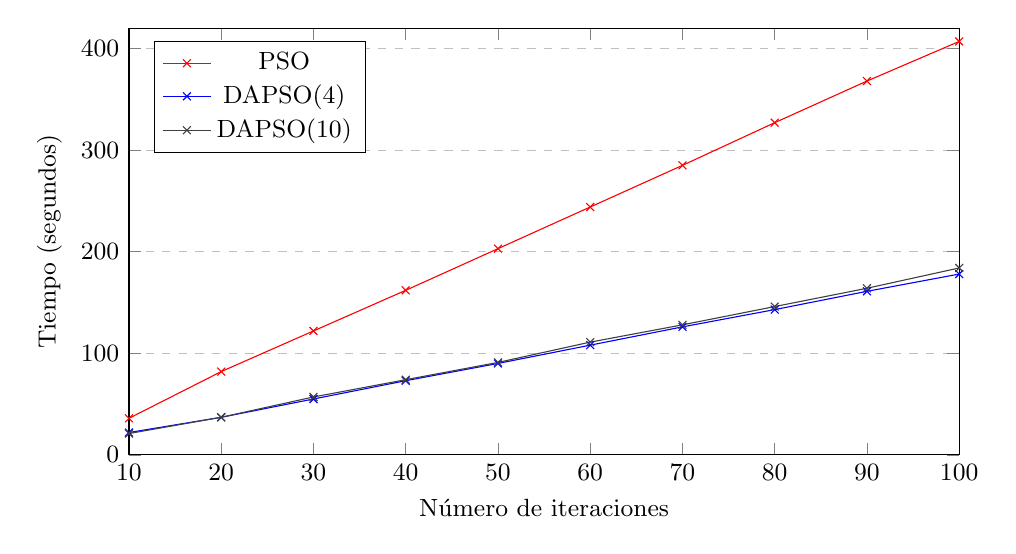
\begin{tikzpicture}[font=\small]
\begin{axis}[
    width=\textwidth,
    height=7cm,
    xlabel={Número de iteraciones},
    ylabel={Tiempo (segundos)},
    xmin=10, xmax=100,
    ymin=0, ymax=420,
    legend pos=north west,
    ymajorgrids=true,
    grid style=dashed,
]

\addplot[
    color=red,
    mark=x,
    ]
    coordinates {
    (10,36.0)(20,82.0)(30,122.0)(40,162.0)(50,203.0)(60,244.0)(70,285.0)(80,327.0)(90,368.0)(100,407.0)
    };

\addplot[
    color=blue,
    mark=x,
    ]
    coordinates {
    (10,22.0)(20,37.0)(30,55.0)(40,73.0)(50,90.0)(60,108.0)(70,126.0)(80,143.0)(90,161.0)(100,178.0)
    };
\addplot[
    color=darkgray,
    mark=x,
    ]
    coordinates {
    (10, 21.0)(20, 37.0)(30, 57.0)(40, 74.0)(50, 91.0)(60, 111.0)(70, 128.0)(80, 146.0)(90, 164.0)(100, 184.0)
    };
\legend{PSO, DAPSO(4), DAPSO(10)}
\end{axis}
\end{tikzpicture}
\end{minipage}%
\begin{minipage}[c]{.5\textwidth}
\resizebox{\textwidth}{!}{%
\raggedleft
    \begin{tabular}{c|ccc}
    \textbf{Nº de} & \multicolumn{3}{c}{\textbf{Tiempo de ejecución ($s$)}} \\ \cline{2-4} 
    \textbf{iters.} & \textit{PSO} & \textit{DAPSO(4)} & \textit{DAPSO(10)} \\ \hline
    10 & 36 & 22 & 21 \\
    20 & 82 & 37 & 37 \\
    30 & 122 & 55 & 57 \\
    40 & 162 & 73 & 74 \\
    50 & 203 & 90 & 91 \\
    60 & 244 & 108 & 111 \\
    70 & 285 & 126 & 128 \\
    80 & 327 & 143 & 146 \\
    90 & 368 & 161 & 164 \\
    100 & 407 & 178 & 184 \\
    \end{tabular}
}
\end{minipage}
    \caption{Comparativa en tiempo de entrenamiento del PSO secuencial y los distintos DAPSO en un problema de clasificación.}
    \label{fig:comp-tiempo-md}
\end{figure}

\begin{figure}[ht!]
\begin{minipage}[c]{.33\textwidth}
\resizebox{0.9\textwidth}{!}{%
    \renewcommand{\arraystretch}{2}
    \begin{tabular}{ll|x{0.8cm}|x{0.8cm}|}        
\multicolumn{2}{c}{}&   \multicolumn{2}{c}{Predicciones}\\
        \multicolumn{2}{c}{}&\multicolumn{1}{c}{\rotatebox[origin=c]{0}{Pos.}} & \multicolumn{1}{c}{\rotatebox[origin=c]{0}{Neg.}}\\
        \cline{3-4}
        \multirow{2}{*}{{\rotatebox[origin=c]{90}{Etiquetas}
        }} & 
        Pos. & 18 & 8  \\ \cline{3-4}
        &  Neg. & 14 & 74 \\ \cline{3-4}
    \end{tabular}
}
\end{minipage}%
\begin{minipage}[c]{.33\textwidth}
\resizebox{0.9\textwidth}{!}{%
    \centering
    \renewcommand{\arraystretch}{2}
    \begin{tabular}{ll|x{0.8cm}|x{0.8cm}|}        
\multicolumn{2}{c}{}&   \multicolumn{2}{c}{Predicciones}\\
        \multicolumn{2}{c}{}&\multicolumn{1}{c}{\rotatebox[origin=c]{0}{Pos.}} & \multicolumn{1}{c}{\rotatebox[origin=c]{0}{Neg.}}\\
        \cline{3-4}
        \multirow{2}{*}{{\rotatebox[origin=c]{90}{Etiquetas}
        }} & 
        Pos. & 23 & 3  \\ \cline{3-4}
        &  Neg. & 12 & 76 \\ \cline{3-4}
    \end{tabular}
}
\end{minipage}%
\begin{minipage}[c]{.33\textwidth}
\resizebox{0.9\textwidth}{!}{%
    \centering
    \renewcommand{\arraystretch}{2}
    \begin{tabular}{ll|x{0.8cm}|x{0.8cm}|}        
\multicolumn{2}{c}{}&   \multicolumn{2}{c}{Predicciones}\\
        \multicolumn{2}{c}{}&\multicolumn{1}{c}{\rotatebox[origin=c]{0}{Pos.}} & \multicolumn{1}{c}{\rotatebox[origin=c]{0}{Neg.}}\\
        \cline{3-4}
        \multirow{2}{*}{{\rotatebox[origin=c]{90}{Etiquetas}
        }} & 
        Pos. & 22 & 4  \\ \cline{3-4}
        &  Neg. & 9 & 79 \\ \cline{3-4}
    \end{tabular}
}
\end{minipage}
    \caption{Matrices de confusión de los clasificadores entrenados con 100 iteraciones por un algoritmo PSO, DAPSO con
    4 SuperRDDs y DAPSO con 10 SuperRDDs respectivamente.}
    \label{fig:conf-mat-prueba}
\end{figure}

\vspace{10pt}
Veamos ahora la comparativa en cuanto a la exactitud cuando se entrenaron con 100 iteraciones del algoritmo. Podemos 
observar las matrices de confusión de cada una de las redes en la figura \ref{fig:conf-mat-prueba}. Calculamos ahora las 
medidas mencionadas en el \autoref{chap:ann} para cada uno de los clasificadores a partir de esas matrices:

\begin{minipage}[c]{.33\textwidth}
\subsubsection*{Clasificador con algoritmo PSO}
\begin{itemize}
    \item \textit{Exactitud}: 0.8070
    \item \textit{Precisión}: 0.5625
    \item \textit{Sensibilidad}: 0.6923
    \item \textit{Puntuación $f_1$}: 0.3103
\end{itemize}
\end{minipage}%
\begin{minipage}[c]{.33\textwidth}
\subsubsection*{Clasificador con algoritmo DAPSO (4 SuperRDDs)}
\begin{itemize}
    \item \textit{Exactitud}: 0.8684
    \item \textit{Precisión}: 0.6571
    \item \textit{Sensibilidad}: 0.8846
    \item \textit{Puntuación $f_1$}: 0.3770
\end{itemize}
\end{minipage}%
\begin{minipage}[c]{.33\textwidth}
\subsubsection*{Clasificador con algoritmo DAPSO (10 SuperRDDs)}
\begin{itemize}
    \item \textit{Exactitud}: 0.8860
    \item \textit{Precisión}: 0.7097
    \item \textit{Sensibilidad}: 0.8846
    \item \textit{Puntuación $f_1$}: 0.3938
\end{itemize}
\end{minipage}%

\vspace{10pt}
Observamos cómo la versión distribuida proporciona mejores resultados en todas las medidas. Al tratarse de un modelo que
intenta predecir casos de cáncer, la mejora de sensibilidad de casi 0.2 al utilizar el algoritmo DAPSO es crucial. Para 
este problema, la mayor exploración del espacio de búsqueda lograda con la asíncronía, tal y como se describía en
\cite{dapso}, beneficia al modelo.

\vspace{10pt}
La segunda prueba nos servirá para validar los regresores implementados en la librería. Para ello, vamos a utilizar como
conjunto de datos los datos de consumo eléctrico de varios edificios de la Universidad de Granada. Para ello, vamos a
construir dos redes con 15 neuronas de entrada y 30 neuronas ocultas, y entrenaremos esas redes mediante un algoritmo PSO
y un algoritmo DAPSO respectivamente. Los parámetros de los algoritmos y las redes se encuentran especificados en la tabla
\ref{tab:conf-2}.

\vspace{10pt}
Un resumen visual de esta prueba puede encontrarse en la figura \ref{fig:comp-reg}. Una vez más, observamos que el 
algoritmo DAPSO tiene un tiempo de ejecución más de dos veces menor que su contraparte secuencial. La diferencia en este 
caso es más acusada (420 frente a 184 en el clasificador y 861 frente a 313 en el regresor), y se atribuye al aumento del
tamaño de la muestra (456 frente a 3000), mostrando de esta manera la mayor capacidad de escalabilidad que tiene el modelo
que utiliza un algoritmo sobre Spark. Esta capacidad aumentada la desarrollaremos más en la siguiente prueba.

\begin{table}[ht!]
    \centering
    \begin{tabular}{x{0.5\textwidth}x{0.3\textwidth}}
    \hline
    \textbf{Parámetro} & \textbf{Valor} \\
    \hline
    Tamaño de la muestra de entrenamiento & 3000 \\
    Iteraciones & 10, 20, 30, 40, 50, 60, 70, 80, 90, 100 \\
    Nº de neuronas en la capa de entrada & 15 \\
    Nº de neuronas en la capa oculta & 30 \\
    Nº de partículas PSO y DAPSO & 100 \\
    SuperRDDs & 4 \\
    Tamaño de los lotes & 10 \\
    Intervalo de posiciones & [-1,1] \\
    Intervalo de velocidades & [-0.6,0.6] (0.6$\times\text{pos max}$) \\
    $w$ & 1 \\
    $c_1$ & 0.8 \\
    $c_2$ & 0.2 \\
    \hline
    \end{tabular}
    \caption{Configuración de parámetros para la segunda prueba.}
    \label{tab:conf-2}
\end{table}

\begin{figure}[ht!]
\begin{minipage}[c]{.5\textwidth}
\raggedright
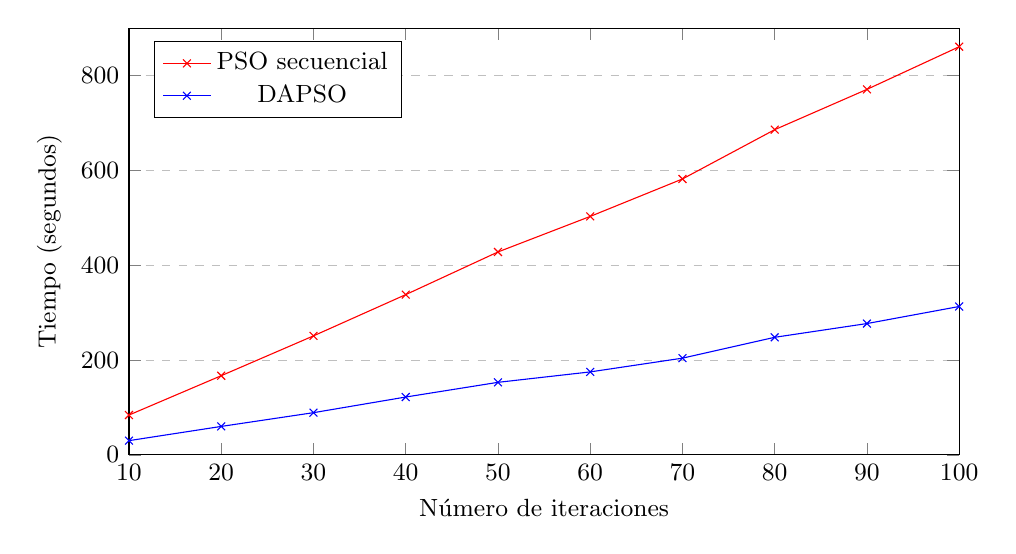
\begin{tikzpicture}[font=\small]
\begin{axis}[
    width=\textwidth,
    height=7cm,
    xlabel={Número de iteraciones},
    ylabel={Tiempo (segundos)},
    xmin=10, xmax=100,
    ymin=0, ymax=900,
    legend pos=north west,
    ymajorgrids=true,
    grid style=dashed,
]

\addplot[
    color=red,
    mark=x,
    ]
    coordinates {
    (10, 84.0)(20, 167.0)(30, 251.0)(40, 338.0)(50, 428.0)(60, 503.0)(70, 582.0)(80, 686.0)(90, 771.0)(100, 861.0)
    };
\addplot[
    color=blue,
    mark=x,
    ]
    coordinates {
    (10, 30.0)(20, 60.0)(30, 89.0)(40, 122.0)(50, 153.0)(60, 175.0)(70, 204.0)(80, 248.0)(90, 277.0)(100, 313.0)
    };
\legend{PSO secuencial, DAPSO}
\end{axis}
\end{tikzpicture}
\end{minipage}%
\begin{minipage}[c]{.5\textwidth}
\resizebox{\textwidth}{!}{%
\raggedleft
    \begin{tabular}{c|cc}
    \textbf{Nº de} & \multicolumn{2}{c}{\textbf{Tiempo ejecución ($s$)}} \\ \cline{2-3} 
    \textbf{iters} & \textit{PSO} & \textit{DAPSO} \\ \hline
10 & 84 & 30 \\
20 & 167 & 60 \\
30 & 251 & 89 \\
40 & 338 & 122 \\
50 & 428 & 153 \\
60 & 503 & 175 \\
70 & 582 & 204 \\
80 & 686 & 248 \\
90 & 771 & 277 \\
100 & 861 & 313 \\
    \end{tabular}
}
\end{minipage}
    \caption{Comparativa en tiempo de entrenamiento del PSO secuencial y el DAPSO para un problema de regresión.}
    \label{fig:comp-reg}
\end{figure}

\vspace{10pt}
En cuanto a la calidad de los resultados, podemos ver en la tabla \ref{tab:reg-mse} que en este caso el algoritmo DAPSO
se comporta peor que el secuencial. Estos difieren mucho de los obtenidos en 
\cite{iruela_ruiz_criado-ramón_pegalajar_capel_2024} (origen del conjunto de datos), pero lo podemos atribuir al tamaño
de la muestra escogido (3000) y el mínimo preprocesamiento de los datos. De cualquier manera, hemos comprobado el correcto
funcionamiento de los regresores en la librería.

\begin{table}[ht!]
    \centering
    \resizebox{\textwidth}{!}{%
\begin{tabular}{c|cccccccccc}
\textbf{Algoritmo de} & \multicolumn{10}{c}{\textbf{Iteraciones}} \\ \cline{2-11} 
\textbf{entrenamiento} & 10 & 20 & 30 & 40 & 50 & 60 & 70 & 80 & 90 & 100 \\ \hline
\textit{PSO secuencial} & 476.284 & 476.284 & 476.284 & 460.355 & 460.355 & 460.355 & 460.355 & 447.481 & 447.481 & 447.481
  \\
\textit{DAPSO} & 800.451 & 800.451 & 800.451 & 800.451 & 800.451 & 800.451 & 800.451 & 800.451 & 800.451 & 800.451
\end{tabular}
}
    \caption{Error cuadrático medio de los regresores para las distintas iteraciones.}
    \label{tab:reg-mse}
\end{table}

\vspace{10pt}
La tercera y última prueba a realizar viene a mostrar la capacidad de escalabilidad de la solución distribuida. Para ello 
usaremos un conjunto de datos de entrenamiento más grande, relacionado con los casos de COVID-19, y compararemos el 
tiempo de ejecución del algoritmo de entrenamiento frente a la cantidad de ejemplos utilizados en el proceso. Creamos 
para ello dos redes neuronales, que utilizarán una el PSO secuencial y la otra el DAPSO. Los parámetros para estos dos 
algoritmos serán los mismos que los utilizados para la prueba anterior, a excepción del número de partículas, que será 
ahora 50. En cuanto a las redes, ambas tendrán 23 neuronas en la capa de entrada y 46 en la de salida, y se entrenarán 
con 50 iteraciones. Un resumen de los parámetros lo podemos encontrar en la tabla \ref{tab:conf-3}.

\begin{table}[ht!]
    \centering
    \begin{tabular}{x{0.5\textwidth}x{0.3\textwidth}}
    \hline
    \textbf{Parámetro} & \textbf{Valor} \\
    \hline
    Tamaño de la muestra de entrenamiento & 500, 1000, 1500, 2000, 2500, 3000, 3500, 4000, 4500, 5000 \\
    Iteraciones & 50 \\
    Nº de neuronas en la capa de entrada & 23 \\
    Nº de neuronas en la capa oculta & 50 \\
    Nº de partículas PSO y DAPSO & 50 \\
    SuperRDDs & 4 \\
    Tamaño de los lotes & 10 \\
    Intervalo de posiciones & [-1,1] \\
    Intervalo de velocidades & [-0.6,0.6] (0.6$\times\text{pos max}$) \\
    $w$ & 0.721 ($\frac{1}{2\ln{2}}$) \\
    $c_1$, $c_2$ & 1.193 ($\frac 12+\ln{2}$) \\
    \hline
    \end{tabular}
    \caption{Configuración de parámetros para la tercera prueba.}
    \label{tab:conf-3}
\end{table}

\vspace{10pt}
El resultado de esta prueba se encuentra en la figura \ref{fig:comp-tiempo-dd}. Podemos apreciar claramente el beneficio 
que aporta el uso de algoritmos distribuidos y Spark en este caso. Conforme aumentamos el número de datos utilizados 
durante el entrenamiento, la diferencia en el tiempo de ejecución para el algoritmo secuencial y el paralelo aumenta a 
una gran velocidad. En particular, el algoritmo DAPSO es ya el doble de rápido (64 segundos frente a 32 segundos) cuando
el tamaño de la muestra es de únicamente 500 ejemplos, llegando a más del triple (824 segundos frente a 264 segundos) 
cuando la muestra contiene 5000 ejemplos.

\begin{figure}[ht!]
\begin{minipage}[c]{.5\textwidth}
\raggedright
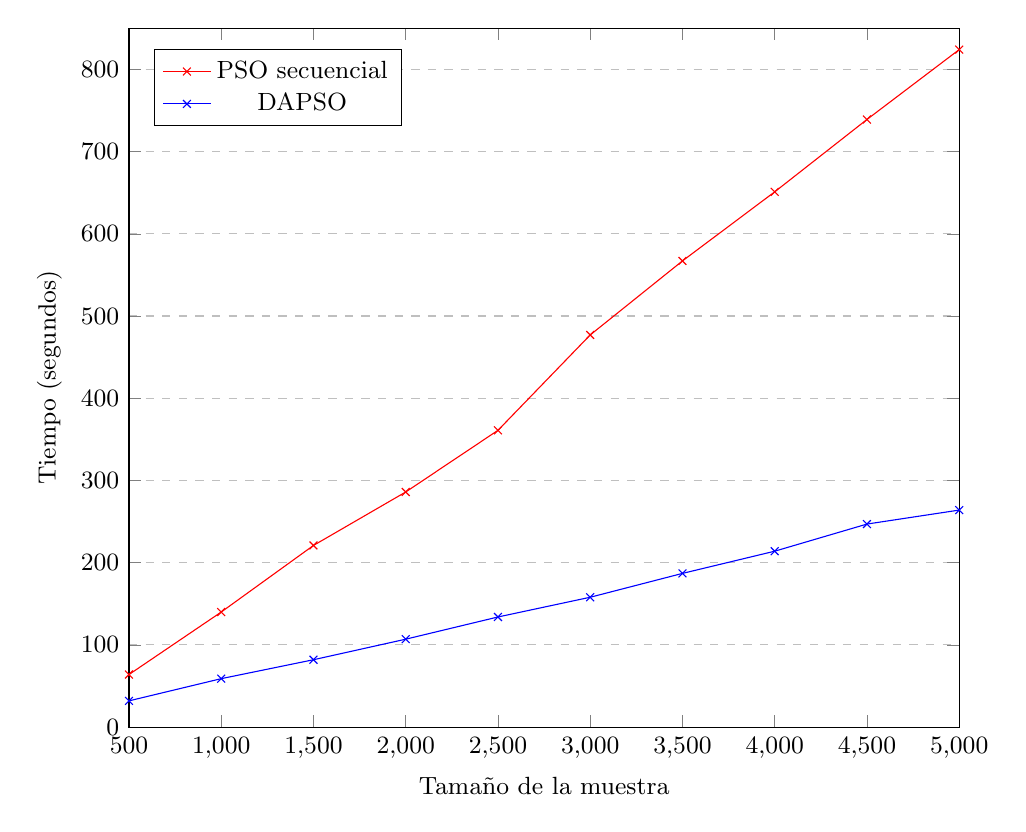
\begin{tikzpicture}[font=\small]
\begin{axis}[
    width=\textwidth,
    xlabel={Tamaño de la muestra},
    ylabel={Tiempo (segundos)},
    xmin=500, xmax=5000,
    ymin=0, ymax=850,
    legend pos=north west,
    ymajorgrids=true,
    grid style=dashed,
]

\addplot[
    color=red,
    mark=x,
    ]
    coordinates {
    (500, 64.0)(1000, 140.0)(1500, 221.0)(2000, 286.0)(2500, 361.0)(3000, 477.0)(3500, 567.0)(4000, 651.0)(4500, 739.0)(5000, 824.0)
    };
\addplot[
    color=blue,
    mark=x,
    ]
    coordinates {
    (500, 32.0)(1000, 59.0)(1500, 82.0)(2000, 107.0)(2500, 134.0)(3000, 158.0)(3500, 187.0)(4000, 214.0)(4500, 247.0)(5000, 264.0)

    };
\legend{PSO secuencial, DAPSO}
\end{axis}
\end{tikzpicture}
\end{minipage}%
\begin{minipage}[c]{.5\textwidth}
\resizebox{\textwidth}{!}{%
\raggedleft
    \begin{tabular}{c|cc}
    \textbf{Tamaño de} & \multicolumn{2}{c}{\textbf{Tiempo ejecución ($s$)}} \\ \cline{2-3} 
    \textbf{la muestra} & \textit{PSO} & \textit{DAPSO} \\ \hline
    500 & 64 & 32 \\
    1000 & 140 & 59 \\
    1500 & 221 & 82 \\
    2000 & 286 & 107 \\
    2500 & 361 & 134 \\
    3000 & 477 & 158 \\
    3500 & 567 & 187 \\
    4000 & 651 & 214 \\
    4500 & 739 & 247 \\
    5000 & 824 & 264 \\
    \end{tabular}
}
\end{minipage}
    \caption{Comparativa en tiempo de entrenamiento del PSO secuencial y el DAPSO para diferentes muestras de entrenamiento.}
    \label{fig:comp-tiempo-dd}
\end{figure}

\vspace{10pt}
En definitiva, hemos comprobado el correcto funcionamiento, mediante estas tres pruebas, de la librería implementada en el
proyecto. También hemos comprobado la mejora sustancial en tiempos de ejecución del algoritmo DAPSO, mostrando también sus
altas capacidades de escalabilidad al aumentar el tamaño de la muestra con la que se trabaja, proporcionando así una 
solución al problema presentado en la introducción.

\section{Intérprete}

Vamos a mostrar el analizador léxico y el explorador del intérprete de SSDL creado. A partir de unas piezas de código,
mostraremos la lista de \textit{tokens} generada y el árbol de sintaxis abstracta generado.

\vspace{10pt}
Comenzamos con la descripción de un algoritmo DAPSO. La pieza de código que lo genera es la siguiente
(figura \ref{fig:dapso-ssdl}):

\begin{figure}[ht!]
    \centering
    \StartLineAt{1}
    \lstinputlisting[language=Pascal]{code/dapso.ssdl}
    \caption{Código en SSDL para la configuración de un algoritmo DAPSO}
    \label{fig:dapso-ssdl}
\end{figure}

El analizador léxico del lenguaje genera, para esa secuencia, los siguientes \textit{tokens}:
\vspace{10pt}
\begin{lstlisting}[numbers=none]
[@0,29:33='begin',<'begin'>,2:0]
[@1,35:39='dapso',<OBJECT>,2:6]
[@2,40:40=':',<':'>,2:11]
[@3,42:46='DAPSO',<ID>,2:13]
[@4,52:54='set',<'set'>,3:4]
[@5,56:64='particles',<'particles'>,3:8]
[@6,66:67='50',<INT>,3:18]
[@7,73:75='set',<'set'>,4:4]
[@8,77:85='pos_bound',<'pos_bound'>,4:8]
[@9,87:89='2.0',<FLOAT>,4:18]
[@10,95:97='set',<'set'>,5:4]
[@11,99:108='batch_size',<'batch_size'>,5:8]
[@12,110:111='10',<INT>,5:19]
[@13,113:115='end',<'end'>,6:0]
[@14,116:115='<EOF>',<EOF>,6:3]
\end{lstlisting}

Podemos ver que los comentarios, al no generar ninguna sentencia, son ignorados por el analizador, simplificando 
en adelante el árbol de sintaxis abstracta. Veamos ahora el árbol de sintaxis abstracta o AST del programa (figura 
\ref{fig:dapso-ast}):

\begin{figure}[ht!]
    \centering
    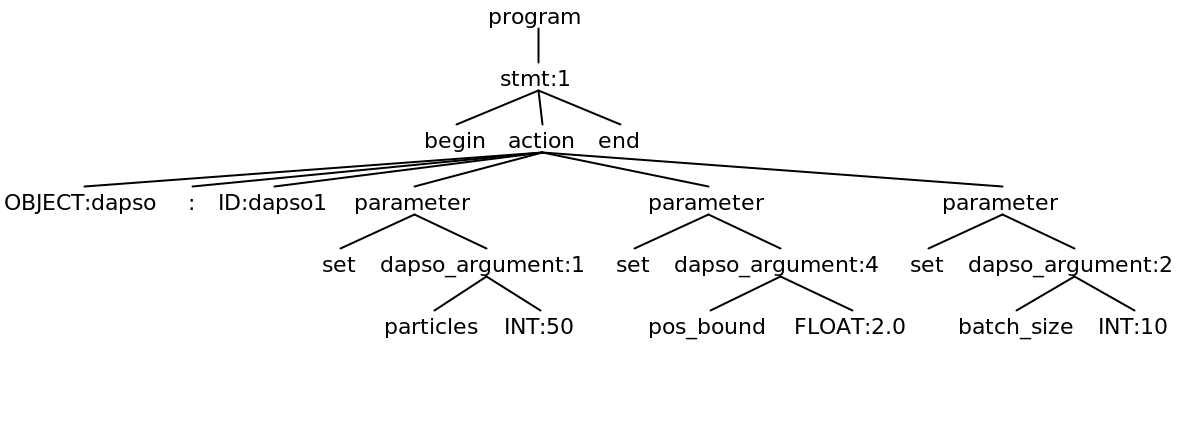
\includegraphics[width=1\linewidth]{img/dapso_ast.png}
    \caption{AST para la configuración de un algoritmo DAPSO.}
    \label{fig:dapso-ast}
\end{figure}

\vspace{10pt}
El código que generaría el intérprete a partir del AST, usando la librería implementada sería el de la figura 
\ref{fig:dapso-ssdl-scala}.

\vspace{10pt}
\begin{figure}[ht!]
    \StartLineAt{1}
    \begin{lstlisting}[language=Scala]
val dapso1 = new DAPSO(50, 2.0, batchSize = 10)
    \end{lstlisting}
    \caption{Código en Scala equivalente a la especificación en SSDL de la figura \ref{fig:dapso-ast}.}
    \label{fig:dapso-ssdl-scala}
\end{figure}

Veamos ahora una pieza de código más compleja. Supongamos que, después del código mostrado anteriormente, encontramos el 
siguiente código (figura \ref{fig:ann-ssdl}):

\begin{figure}[ht!]
    \centering
    \StartLineAt{7}
    \lstinputlisting[language=Pascal]{code/ann.ssdl}
    \caption{Código en SSDL para la configuración, entrenamiento y exportación de datos de una red neuronal.}
    \label{fig:ann-ssdl}
\end{figure}

El analizador léxico creado extrae la siguiente lista de \textit{tokens}:
\vspace{10pt}
\begin{lstlisting}[numbers=none]
[@0,36:40='begin',<'begin'>,2:0]
[@1,42:44='ann',<OBJECT>,2:6]
[@2,45:45=':',<':'>,2:9]
[@3,47:51='clas1',<ID>,2:11]
[@4,57:59='set',<'set'>,3:4]
[@5,61:64='type',<'type'>,3:8]
[@6,66:75='classifier',<NET_TYPE>,3:13]
[@7,81:83='set',<'set'>,4:4]
[@8,85:91='neurons',<'neurons'>,4:8]
[@9,93:93='[',<'['>,4:16]
[@10,94:95='50',<INT>,4:17]
[@11,96:96=',',<','>,4:19]
[@12,97:99='200',<INT>,4:20]
[@13,100:100=']',<']'>,4:23]
[@14,106:108='set',<'set'>,5:4]
[@15,110:113='data',<'data'>,5:8]
[@16,115:115='[',<'['>,5:13]
[@17,116:135='"covid_training.csv"',<FILE>,5:14]
[@18,136:136=',',<','>,5:34]
[@19,137:152='"covid_test.csv"',<FILE>,5:35]
[@20,153:153=']',<']'>,5:51]
[@21,159:161='set',<'set'>,6:4]
[@22,163:171='algorithm',<'algorithm'>,6:8]
[@23,173:177='DAPSO',<ID>,6:18]
[@24,179:181='end',<'end'>,7:0]
[@25,203:205='fit',<'fit'>,9:0]
[@26,207:211='clas1',<ID>,9:4]
[@27,213:215='100',<INT>,9:10]
[@28,217:219='out',<'out'>,10:0]
[@29,221:225='clas1',<ID>,10:4]
[@30,227:248='"clasificador_100.csv"',<FILE>,10:10]
[@31,249:248='<EOF>',<EOF>,10:32]
\end{lstlisting}

Generando a partir de ella el explorador el AST siguiente (figura \ref{fig:ann-ast}):

\begin{figure}[ht!]
    \centering
    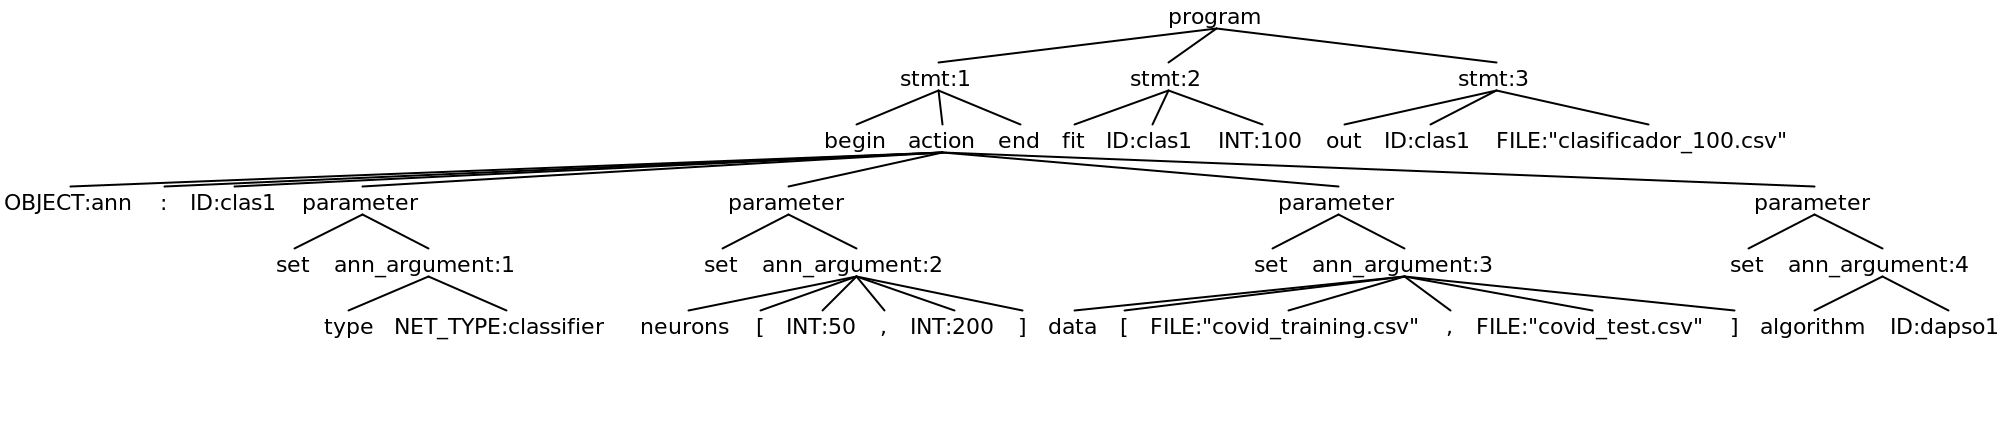
\includegraphics[width=1\linewidth]{img/ann_ast.png}
    \caption{AST para la configuración, entrenamiento y exportación de pesos de una red neuronal.}
    \label{fig:ann-ast}
\end{figure}

Unificando este AST con el anterior, obtenemos un programa completo que especifica los parámetros de un algoritmo DAPSO,
configura una red neuronal con ese algoritmo, la entrena y exporta los pesos obtenidos de ese entrenamiento. El código que
el intérprete escribiría a partir del árbol aparece en la figura \ref{fig:ssdl-scala}.

\vspace{10pt}
\begin{figure}[ht!]
    \centering
    \StartLineAt{1}
    \begin{lstlisting}[language=Scala]
val dapso1 = new DAPSO(50, 2.0, batchSize = 10)

val clas1 = new Classifier(50,200)
clas1.setTrainingData("covid_training.csv", Int.MaxValue)
clas1.setTestData("covid_test.csv", Int.MaxValue)
clas1.setTrainer(dapso1)

clas1.fit(100)
clas1.writeWeights("clasificador_100.csv")
    \end{lstlisting}
    \caption{Código en Scala equivalente a la especificación en SSDL de las figuras \ref{fig:dapso-ast} y \ref{fig:ann-ast}.}
    \label{fig:ssdl-scala}
\end{figure}

\endinput
%--------------------------------------------------------------------
% FIN DEL CAPÍTULO. 
%--------------------------------------------------------------------

% !TeX root = ../tfg.tex
% !TeX encoding = utf8

\chapter{Conclusiones}

Al terminar el trabajo, quedan algunos objetivos por cumplir, principalmente la finalización del intérprete. Sin embargo,
se ha conseguido realizar, en primer lugar, una librería en Scala que permite automatizar el proceso de aprendizaje de
redes neuronales mediante algoritmos distribuidos. También se ha conseguido generar una gramática para el lenguaje de la
herramienta, así como el analizador léxico y el \textit{parser} del intérprete.

\vspace{10pt}
Es interesante resaltar la diferencia en la sintaxis de ese lenguaje frente al usual para las técnicas de ML, Python.
Las restricciones que presenta Scala con su tipado fuerte, frente al de Python, junto con el énfasis de Scala en la
inmutabilidad y el paradigma de programación funcional, parecen resultar, más que un impedimento, una ayuda involuntaria
para mejorar la fiabilidad de un modelo de aprendizaje automático. Para las redes neuronales, que presentan una cierta
complejidad a la hora de su configuración y requieren una inversión en tiempo para su entrenamiento, es importante
asegurarse de la validez del código escrito antes de su funcionamiento. Es por ello que un lenguaje como Scala, que
requiere de un trabajo previo a la ejecución más concienzudo puede ser un buen candidato como lenguaje a utilizar para
el aprendizaje automático.

\vspace{10pt}
La aproximación a los lenguajes de programación y los intérpretes desde un punto de vista formal ha dado una visión distinta
del funcionamiento y componentes de los mismos. El visualizar un lenguaje de programación como el generado por una gramática
libre de contexto permite entenderlos desde una perspectiva más abstracta que permite entender los patrones generales de
diseño de los mismos.

\vspace{10pt}
Finalmente, cabe destacar que el objetivo último de este trabajo es intentar democratizar de alguna manera las técnicas de
ML para su uso por personas sin conocimientos específicos. Dada la tendencia actual de adopción en masa por todos los
sectores de la sociedad, una herramienta así puede ser de gran ayuda para limitar el impacto que pueden provocar en las
personas más alejadas de este campo de la ingeniería.

% -------------------------------------------------------------------------------------------------------------------
\section{Futuros trabajos}

Aunque se han alcanzado algunos de los objetivos propuestos, no se ha podido completar la herramienta originalmente
ideada para el problema a resolver. Por tanto, el principal trabajo futuro a realizar es la finalización del intérprete
de SSDL.

\vspace{10pt}
Sería deseable también ampliar el número de algoritmos distribuidos de la librería implementada. Puesto que se ha 
construido una interfaz para ellos, no debería ser muy complicado implementar nuevos algoritmos (sin tener en cuenta la
dificultad de implementación inherente que puedan tener). Para incluirlos en el lenguaje, simplemente tendría que 
expandirse la producción \textlangle object\textrangle, añadiendo en nombre del algoritmo como posible parte derecha y
añadir producciones para los parámetros específicos del mismo.

\vspace{10pt}
De la misma manera, un futuro trabajo podría ser la ampliación de tipos de modelos de aprendizaje automático soportados
por la herramienta. Actualmente solamente es capaz de expresar redes neuronales prealimentadas con una capa oculta, pero
se podría generalizar a redes neuronales prealimentadas, y de ahí a otro tipo de redes más complejas, como las 
convolucionales. El procedimiento para incorporarlas al lenguaje sería similar: habría que expandir de nuevo la producción
de \textlangle object\textrangle, así como crear las producciones con los parámetros específicos de ese tipo de redes.

\endinput
%--------------------------------------------------------------------
% FIN DEL CAPÍTULO. 
%--------------------------------------------------------------------


% -------------------------------------------------------------------
% APPENDIX: Opcional
% -------------------------------------------------------------------

\part{Apéndices}
\appendix % Reinicia la numeración de los capítulos y usa letras para numerarlos
% !TeX root = ../tfg.tex
% !TeX encoding = utf8

\chapter{Estructura redes neuronales}\label{ap:estructura_ann}

No se incluyen en esta muestra de código las sentencias de importación de funciones.

\vspace{10pt}
\StartLineAt{1}
\lstinputlisting[language=Scala,caption={\texttt{ann.scala}}]{code/ann_simplified.scala}
\StartLineAt{1}
\lstinputlisting[language=Scala,caption={\texttt{trainer.scala}}]{code/Trainer.scala}

\endinput
%------------------------------------------------------------------------------------
% FIN DEL APÉNDICE. 
%------------------------------------------------------------------------------------

% !TeX root = ../tfg.tex
% !TeX encoding = utf8

\chapter{Implementación del algoritmo DAPSO}\label{ap:dapso}

\StartLineAt{1}
\lstinputlisting[language=Scala, caption={\texttt{DAPSO.scala}}]{code/DAPSO.scala}
\StartLineAt{1}
\lstinputlisting[language=Scala, caption={\texttt{GlobalActor.scala}}]{code/GlobalActor.scala}
\StartLineAt{1}
\lstinputlisting[language=Scala, caption={\texttt{FitnessActor.scala}}]{code/FitnessActor.scala}
\StartLineAt{1}
\lstinputlisting[language=Scala, caption={\texttt{DAPSOController.scala}}]{code/DAPSOController.scala}
\StartLineAt{1}
\lstinputlisting[language=Scala, caption={\texttt{BatchPSO.scala}}]{code/BatchPSO.scala}

\endinput
%------------------------------------------------------------------------------------
% FIN DEL APÉNDICE. 
%------------------------------------------------------------------------------------

% !TeX root = ../tfg.tex
% !TeX encoding = utf8

\chapter{Programa en SSDL}\label{ap:ejemplo_ssdl}

\StartLineAt{1}
\lstinputlisting[language=Pascal]{code/example.ssdl}

\endinput
%------------------------------------------------------------------------------------
% FIN DEL APÉNDICE. 
%------------------------------------------------------------------------------------

% !TeX root = ../tfg.tex
% !TeX encoding = utf8

\chapter{Gramática del lenguaje en la sintaxis de ANTLR}\label{ap:ssdl_g4}

\StartLineAt{1}
\lstset{ %
  texcl=true,
  escapeinside={//}{\^^M},
}
\begin{lstlisting}[language=Java,texcl=false]
/**
 * GRAMMAR FOR SCALA-SPARK DISTRIBUTED LEARNING
 */
grammar ssdl;
program: (stmt|COMMENT)+;
stmt:
    'begin' action 'end'
    |'fit' ID INT
    |'out' ID FILE?;
action: OBJECT ':' ID parameter+;
parameter: 'set' (ann_argument|dapso_argument);
ann_argument:
    'type' NET_TYPE
    |'neurons' '['INT','INT']'
    |'data' '['FILE','FILE']'
    |'algorithm' ID;
dapso_argument:
    'particles' INT
    |'batch_size' INT
    |'n_rdd' INT
    |'pos_bound' FLOAT
    |'vel_bound' FLOAT
    |'vel_w' FLOAT
    |'vel_c1' FLOAT
    |'vel_c2' FLOAT;
OBJECT: 'ann' | 'dapso';
NET_TYPE: 'classifier' | 'regressor';
COMMENT: '/*' .*? '*/' -> skip;
INT: [0-9]+;
FLOAT: INT '.' INT | INT;
ID: [a-zA-Z0-9]+;
FILE: '"'.+?'.csv"';
WS: [ \t\r\n]+ -> skip;
\end{lstlisting}

\endinput
%------------------------------------------------------------------------------------
% FIN DEL APÉNDICE. 
%------------------------------------------------------------------------------------

% \input{apendices/apendice-ejemplo}
% Añadir tantos apéndices como sea necesario 

% -------------------------------------------------------------------
% BACKMATTER
% -------------------------------------------------------------------

% \backmatter % Desactiva la numeración de los capítulos
% \pdfbookmark[-1]{Referencias}{BM-Referencias}

% BIBLIOGRAFÍA
%-------------------------------------------------------------------

\bibliographystyle{alpha-es} 
\begin{small} 
  \bibliography{library.bib}
\end{small}


\end{document}
